% Plantilla TFG LaTeX LSI por:
%   Agustín Borrego <borrego@us.es>
%   Inma Hernández <inmahernandez@us.es>
% Su uso y modificación es libre.

% ̀¡Recuerda hacer copias de seguridad frecuentes durante la redacción del trabajo!
% Puedes descargar todo el código fuente del proyecto en zip en Menú > (Descargar) Fuente

\documentclass[12pt]{report}

% Paquetes LaTeX y estilos globales
\usepackage[utf8]{inputenc}
\usepackage{multicol}
\usepackage{xcolor}
\usepackage{subfigure}
\usepackage[spanish,es-tabla]{babel}
\usepackage[utf8]{inputenc}
\usepackage{graphicx}
\usepackage{titlesec}
\usepackage[bookmarks,breaklinks,colorlinks=true,allcolors=blue]{hyperref}
\usepackage{listings}
\usepackage{inconsolata}
\usepackage{float}
\usepackage{mathpazo} % Fuente Palatino
\usepackage[labelfont=bf]{caption}

\usepackage[square,numbers]{natbib}
\usepackage[nottoc,notlof,notlot]{tocbibind}  % Mete la bibliografía como capítulo en la TOC, los parámetros excluyen los otros índices de aparecer también
\usepackage{geometry}
\usepackage{amsmath}
\usepackage{parskip}
\usepackage[official]{eurosym}
\usepackage{todonotes}
\usepackage{csquotes}
\usepackage{tocbasic}  % Estilos de la TOC

% Formato del título de capítulos y secciones
\titleformat{\chapter}[block]{\normalfont\huge\bfseries}{\thechapter.}{.5em}{\Huge}[\vspace{2pt}{\titlerule[2pt]}]

\titlespacing*{\chapter}{0pt}{-19pt}{25pt}

\titleformat{\section}[block]{\normalfont\Large\bfseries}{\thesection.}{.5em}{\Large}

\titleformat{\part}[block]{\titlerule[2pt]\normalfont\Huge\bfseries\centering}{Parte \Roman{part}\\\vspace{15pt}}{0pt}{\Huge}[\vspace{2pt}{\titlerule[2pt]}]

% Tamaños y estilos de elementos en la TOC
\DeclareTOCStyleEntry[
    linefill=\bfseries\TOCLineLeaderFill,
    beforeskip=12pt,
    entrynumberformat=\chapterprefixintoc,
    entryformat=\chaptertocformat,
    pagenumberformat=\chaptertocformat,
    dynnumwidth
]{tocline}{chapter}

\DeclareTOCStyleEntry[
    % linefill=\bfseries\TOCLineLeaderFill,
    beforeskip=30pt,
    entrynumberformat=\chapterprefixintoc,
    entryformat=\parttocformat,
    pagenumberformat=\partpagetocformat,
    numwidth=0pt
]{tocline}{part}

\newcommand\chaptertocformat[1]{\large{\textbf{#1}}}%
\newcommand\chapterprefixintoc[1]{#1}%
\newcommand\parttocformat[1]{\Large{\textbf{#1}}}%
\newcommand\partpagetocformat[1]{} % Don't print the page number for parts

% Alias para estilos de texto comunes
\newcommand{\negritas}[1]{\textbf{#1}}
\newcommand{\cursiva}[1]{\textit{#1}}
\newcommand{\codigo}[1]{\texttt{#1}}

% Formato del código fuente con lstlisting
\lstset{
  basicstyle=\ttfamily,
  breaklines=true,
}

% Márgenes
\geometry{
    a4paper,
    margin=2.75cm
}
\setlength{\marginparwidth}{2cm} 

% Limite de profundidad del índice
\setcounter{tocdepth}{2}

% Eliminar el guionado
\tolerance=1
\emergencystretch=\maxdimen
\hyphenpenalty=10000
\hbadness=10000

% Indentación de párrafos
\setlength{\parindent}{.75cm}

\renewcommand{\lstlistingname}{Extracto de código}
\renewcommand*{\lstlistlistingname}{Índice de extractos de código}

% Comandos para establecer variables
\newcommand{\setTitle}[1]{\def\tfgTitle {#1}}
\newcommand{\setAuthor}[1]{\def\tfgAuthors {#1}}
\newcommand{\setDegree}[1]{\def\tfgDegree {#1}}
\newcommand{\setSupervisor}[1]{\def\tfgSupervisor {#1}}
\newcommand{\setDepartment}[1]{\def\tfgDepartment {#1}}
\newcommand{\setMonth}[1]{\def\tfgMonth {#1}}
\newcommand{\setYear}[1]{\def\tfgYear {#1}}
\newcommand{\setDedication}[1]{\def\tfgDedication {#1}}

% Estilos para el código
% Configuración genérica
\definecolor{codegreen}{rgb}{0,0.6,0}
\definecolor{codegray}{rgb}{0.5,0.5,0.5}
\definecolor{codepurple}{rgb}{0.58,0,0.82}
\definecolor{editorOcher}{rgb}{0.8, 0.3, 0} % #FF7F00 -> rgb(239, 169, 0)
\definecolor{editorGreen}{rgb}{0, 0.5, 0} % #007C00 -> rgb(0, 124, 0)

\lstdefinestyle{listingstyle}{
    backgroundcolor=\color{white},  
    keywordstyle=\bfseries\color{blue},
    numberstyle=\tiny\color{codegray},
    stringstyle=\color{editorGreen},
    commentstyle=\color{codegray},
    basicstyle=\ttfamily\color{black},
    breakatwhitespace=false,         
    breaklines=true,                 
    captionpos=b,                    
    keepspaces=true,                 
    numbers=left,                    
    numbersep=5pt,                  
    showspaces=false,                
    showstringspaces=false,
    showtabs=false,                  
    tabsize=2,
    frame=tb,
    keywords=[2]{True,False},
    literate=%
*{0}{{{\color{editorOcher}0}}}1
{1}{{{\color{editorOcher}1}}}1
{2}{{{\color{editorOcher}2}}}1
{3}{{{\color{editorOcher}3}}}1
{4}{{{\color{editorOcher}4}}}1
{5}{{{\color{editorOcher}5}}}1
{6}{{{\color{editorOcher}6}}}1
{7}{{{\color{editorOcher}7}}}1
{8}{{{\color{editorOcher}8}}}1
{9}{{{\color{editorOcher}9}}}1,
}

\lstset{style=listingstyle}
\lstset{columns=fullflexible}

\lstdefinelanguage{css}{
  keywords={color,background-image:,margin,padding,font,weight,display,position,top,left,right,bottom,list,style,border,size,white,space,min,width, transition:, transform:, transition-property, transition-duration, transition-timing-function},	
  sensitive=true,
  morecomment=[l]{//},
  morecomment=[s]{/*}{*/},
  morestring=[b]',
  morestring=[b]",
  alsoletter={:},
  alsodigit={-}
}
% JavaScript
\lstdefinelanguage{javascript}{
  morekeywords={abstract, arguments, await, boolean, break, byte, case, catch, char, class, const, continue, debugger, default, delete, do, double, else, enum, eval, export, extends, false, final, finally, float, for, function, goto, if, implements, import, in, instanceof, int, interface, let, long, native, new, null, package, private, protected, public, return, short, static, super, switch, synchronized, this, throw, throws, transient, true, try, typeof, var, void, volatile, while, with, yield},
  morecomment=[s]{/*}{*/},
  morecomment=[l]//,
  morestring=[b]",
  morestring=[b]'
}

%Para quitar la sangría al principio de cada párrafo
\setlength{\parindent}{0pt}
%Para dar formato al indice de los enumerados
\usepackage{enumitem}
%Establece el formato ''code'' para código
\newcommand{\code}[1]{\texttt{\textsc{#1}}}
%Para mostrar un encabezado con el capítulo al que pertenece la página
\usepackage{fancyhdr}
\pagestyle{fancy}
\fancyhf{}
\fancyhead[LE,RO]{\slshape \leftmark} %rigthmark muestra la subsec
\fancyfoot[C]{\thepage}
%
\usepackage[nottoc]{tocbibind}
%\usepackage{apacite}
\usepackage[style=apa,backend=biber]{biblatex}
\addbibresource{bibliografia.bib}




%%%%%%%%%%%%%%%%%%%%%%%%%%%%%%%%%%%%%%%%%%%%%%%%%%%%%%%%%%%%%%%%%%%%%%%%%%%%%%%%%%%%%

% Variables para la portada
\setTitle{Estudio y aplicación de la herramienta ATLAS de OHDSI para la estandarización de la investigación clínica}
%Extrayendo conocimiento a partir de análisis clínico de datos CDM usando la herramienta Atlas

%Estandarización y análisis de estudio clínico oncológico mediante OMOP CDM y ATLAS Broadsea

%Estudio y aplicación de la herramienta ATLAS de OHDSI para la investigación clínica

%%%%%%%% {





\setAuthor{Da. María del Valle Alonso de Caso Ortiz} % Si hay más de un autor, separarlos con \\
\setDegree{Grado en Ingeniería de la Salud} % Cambiar si es necesario
\setSupervisor{Dr. Julián Alberto García García \\ Dra. María José Escalona Cuaresma} % Si hay más de un tutor, separarlos con \\
\setDepartment{Lenguajes y Sistemas Informáticos}
\setMonth{junio} % Dejar sólo el mes de la convocatoria en que se presenta el trabajo
\setYear{2023/24} % Por ejemplo, 2022/23

%%%%%%%%%%%%%%%%%%%%%%%%%%%%%%%%%%%%%%%%%%%%%%%%%%%%%%%%%%%%%%%%%%%%%%%%%%%%%%%%%%%%%

% Dedicatoria del trabajo
% Si no se desea incluir, comentar o borrar la línea siguiente para eliminar la página de dedicatoria
\setDedication{A mi padre y a mi madre, por inculcarme la pasión por el estudio y acompañarme incondicionalmente en cada etapa del camino.}

%%%%%%%%%%%%%%%%%%%%%%%%%%%%%%%%%%%%%%%%%%%%%%%%%%%%%%%%%%%%%%%%%%%%%%%%%%%%%%%%%%%%%

% Comienzo del documento
\begin{document}

    % Portada y secciones no numeradas
    \thispagestyle{empty} % Impide que se incluya número de página en la portada
\begin{center}

\vspace*{1cm}


\includegraphics[width=\textwidth]{figures/etsii_us.png}

\vspace*{2.5cm}
\begin{large}
TRABAJO FIN DE GRADO
\end{large}

\vspace*{0.1in}
\textbf{\huge \tfgTitle}

\vspace*{.5in}

{\large Realizado por}\\
\textbf{\Large \tfgAuthors}

\vspace*{2cm}

\textbf{Para la obtención del título de}\\
{\large \tfgDegree}

\vspace*{0.2in}

\textbf{Dirigido por}\\
{\large \tfgSupervisor}\\

\vspace*{0.2in}

\textbf{En el departamento de}\\
{\large \tfgDepartment}

\vspace*{.6in}
\textbf{\Large Convocatoria de \tfgMonth, curso \tfgYear}

\end{center}

% Dedicatoria
\ifdefined\tfgDedication
    \newpage
    \thispagestyle{empty}
    
    \vspace*{\fill}
    \begin{center}
    \textit{\tfgDedication}
    \end{center}
    \vspace*{\fill}
\fi

\clearpage\setcounter{page}{1} % Comienza a incluir números de página a partir de aquí
\pagenumbering{roman} % En números romanos
    \chapter*{Agradecimientos}


    \chapter*{Resumen}
Incluya aquí un resumen de los aspectos generales de su trabajo, en español.

\vspace{.5cm}

\textbf{Palabras clave:} Palabra clave 1, palabra clave 2, ..., palabra clave N
    \chapter*{Abstract}
This section should contain an English version of the Spanish abstract.

\vspace{.5cm}

\textbf{Keywords:} Keyword 1, keyword 2, ..., keyword N
    
    % Índice del documento y de figuras
    \begingroup
        % Los enlaces son normalmente azules, pero en los índices se configuran a negro para que no aparezca todo azul
        \hypersetup{linkcolor=black}
        \tableofcontents
        \listoffigures
        \listoftables
        %\lstlistoflistings
    \endgroup
    
    % Cambia el estilo de números de página de romanos a normal
    \clearpage\pagenumbering{arabic}
    
    % Capítulos del trabajo
    %\chapter{Ejemplos de uso de LaTeX}\label{cap:ejemplos}

\todo[inline]{Este capítulo se incluye únicamente como ayuda y referencia de uso de \LaTeX. No debe aparecer en el documento final.}

\section{Introducción}
En este capítulo se muestran ejemplos de uso de \LaTeX{} para operaciones comunes. 

\section{Estilos}\label{sec:estilos}
Se pueden aplicar estilos al texto como \textbf{negritas}, \textit{cursiva}, \underline{subrayado} y \texttt{monoespaciado}. También se \textcolor{red}{pueden} \textcolor{blue}{aplicar} \textcolor{green}{colores}, y \underline{\textit{combinar}} \textbf{\textcolor{red}{estilos}}. Se recomienda usar sólo negritas para hacer énfasis, y no abusar de este recurso.

Por comodidad para usuarios no habituados con LaTeX, esta plantilla define algunos alias de comandos más fáciles de recordar para estilos de texto comunes: \negritas{negritas}, \cursiva{cursiva} y \codigo{código}.

\section{Listados}
Con itemize se pueden crear listas no numeradas:

\begin{itemize}
    \item Fresas
    \item Melocotones
    \item Piñas
    \item Nectarinas
\end{itemize}

De manera similar, enumerate permite crear listas numeradas:

\begin{enumerate}
    \item Elaborar la memoria del TFG
    \item Elaborar la presentación
    \item Presentar el TFG
    \item Solicitar el título de Grado
\end{enumerate}

\section{Subsecciones}
Se pueden definir subsecciones con el comando \texttt{subsection}:

\subsection{Primera subsección}\label{sec:subseccion}
Esto es una subsección

\subsection{Segunda subsección}
Esto es otra subsección.

\subsubsection{Sub-sub-sección}
Este es un tercer nivel de profundidad, que no aparece en el índice general. Se recomienda no utilizarlo, si es posible.

\section{Imágenes y figuras}
Todas las imágenes y figuras del documento se incluirán en la carpeta ``figures''. Se pueden incluir de la siguiente manera:

\begin{figure}[htp]
    \centering
    
\includegraphics[width=0.7\textwidth]{figures/ejemplo.png}
    \caption{Un feroz depredador}
    \label{fig:ejemplo}
\end{figure}

Observe que las figuras se numeran automáticamente según el capítulo y el número de figuras que hayan aparecido anteriormente en dicho capítulo. Existen muchas maneras de definir el tamaño de una figura, pero se aconseja utilizar la mostrada en este ejemplo: se define el ancho de la figura como un porcentaje del ancho total de la página, y la altura se escala automáticamente. De esta manera, el ancho máximo de una figura sería 1.0 * textwidth, lo que aseguraría que se muestra al máximo tamaño posible sin sobrepasar los márgenes del documento.

Tenga en cuenta que LaTeX intenta incluir las figuras en el mismo sitio donde se declaran, pero en ocasiones no es posible por motivos de espacio. En esos casos, LaTeX colocará la figura lo más cerca posible de su declaración, puede que en una página diferente. Esto es un comportamiento normal.

\section{Tablas}
Existe una gran variedad de formas de crear tablas en LaTeX puro, y todas ellas tienen cierta complejidad. A continuación se muestra un ejemplo simple de tabla nativa, en la Tabla \ref{table:ejemplo}. Se recomienda crear un archivo en la carpeta \textit{tables} por cada tabla nativa que se desee incluir, y enlazarla mediante el comando \texttt{input}.

\begin{table}[htp]
\centering

    % Esta primera línea define las columnas de la tabla. Los posibles tipos de columna son:
    % c: texto centrado
    % l: texto alineado a la izquierda
    % r: texto centrado a la derecha
    % p: columna de ancho fijo
    % Las columnas tienen ancho dinámico según la anchura máxima de los elementos que contengan.

    % Las columnas l/r/c no parten el texto en filas diferentes si éste es demasiado largo. Para ello, puede utilizar el tipo de columna de ancho fijo "p".
    
    % Las barras verticales | se usan para definir los bordes verticales de la tabla. Pruebe a eliminar algunas y observe qué ocurre.
    \begin{tabular}{ | l | c | r | p{2cm} | }
        
        % A continuación van las filas de la tabla. En cada fila, las columnas se separan con el carácter &
        % Para terminar una fila se usa \\
        % Para incluir un borde horizontal entre filas se usa \hline

        % Cabecera con textos en negrita:
        \hline
        \textbf{Columna L} & \textbf{Columna C} & \textbf{Columna R} & \textbf{Columna P}\\
        \hline
        
        % Cuerpo de la tabla:
        Texto de ejemplo & Texto de ejemplo & Texto de ejemplo & Texto de ejemplo\\
        \hline
        ABC & DEF & HIJ & KLM\\
        \hline
        
    \end{tabular} 
    
    \caption{Tabla LaTeX de ejemplo}
    \label{table:ejemplo} 
\end{table}


Para tablas con un formato más complejo, considere la posibilidad de diseñarla usando otro software externo (por ejemplo Excel) e incluirla de manera similar a una figura. \textbf{Observe en el código LaTeX a continuación cómo usar el comando \texttt{captionof\{table\}}, en lugar de simplemente \texttt{caption}, hace que se liste como una Tabla en lugar de como una Figura}:

\begin{figure}[htp]
    \centering
    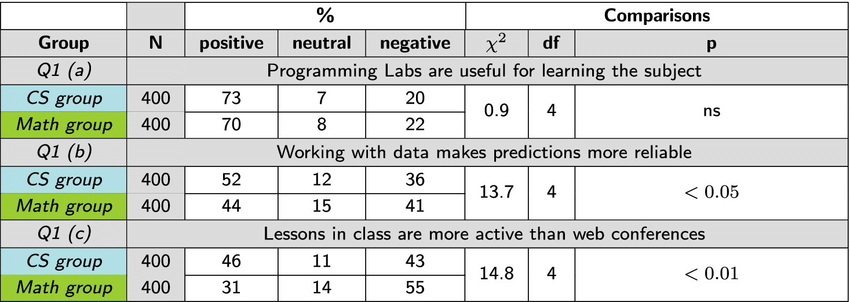
\includegraphics[width=1.0\textwidth]{tables/complex_table.png}
    \captionof{table}{Tabla compleja introducida como figura}
    \label{table:ejemplo2}
\end{figure}

\section{Referencias}
Observe cómo en el código fuente de esta sección se ha usado varias veces el comando \texttt{label}. Este comando permite marcar un elemento, ya sea capítulo, sección, figura, etc. para hacer una referencia numérica al mismo. Para referenciar una label se usa el comando \texttt{ref} incluyendo el nombre de la referencia:

Este es el capítulo \ref{cap:ejemplos}.

En la sección \ref{sec:estilos} se muestran ejemplos de estilos.

La subsección \ref{sec:subseccion} explica...

En la Figura \ref{fig:ejemplo} vemos que...

Esto evita que tengamos que escribir directamente los índices de las secciones y figuras que queremos mencionar, ya que LaTeX lo hace por nosotros y además se encarga de mantenerlos actualizados en caso de que cambien (pruebe a mover este capítulo al final del documento y observe cómo se actualizan automáticamente todos los índices referenciados). Además, las referencias mediante ``ref'' actúan como hipervínculos dentro del documento que llevan al elemento referenciado al pulsar en ellas.

Es habitual nombrar las ``label'' con un prefijo que indica el tipo de elemento para encontrarlo luego más fácilmente, pero no es obligatorio.

\section{Extractos de código}

Se pueden incluir extractos de código mediante lstlisting:

\begin{lstlisting}[language=Python, caption={Código Python}, label={cod:python}, captionpos=b]
num = float(input("Enter a number: "))
if num > 0:
   print("Positive number")
elif num == 0:
   print("Zero")
else:
   print("Negative number")
\end{lstlisting}

Para evitar tener que incluir el código directamente en el texto del documento, se pueden guardar en archivos separados y referenciarlos:

\lstinputlisting[
    float,
    floatplacement=!htp,
    language=Java,
    label=cod:java,
    caption=Código Java
]{code/java_example.java}

\lstinputlisting[
    float,
    floatplacement=!htp,
    language=html,
    label=cod:html,
    caption=Código HTML
]{code/html_example.html}

\lstinputlisting[
    float,
    floatplacement=!htp,
    language=javascript,
    label=cod:js,
    caption=Código JavaScript
]{code/javascript_example.js}

Los extractos de código también se pueden referenciar mediante label/ref: Extractos de código \ref{cod:python}, \ref{cod:java}, \ref{cod:html}, \ref{cod:js}. 

\section{Enlaces}
Puede enlazar una web externa mediante el comando \texttt{url}: \url{https://www.example.com}. También se puede vincular un enlace a un texto mediante el comando href: \href{https://www.example.com}{dominio de ejemplo}.

\section{Citas y bibliografía}
En LaTeX, los elementos de la bibliografía se almacenan en un fichero bibliográfico en un formato llamado BibTeX, en el caso de este proyecto se encuentran en ``bibliografia.bib''. Para citar un elemento se usa el comando \texttt{cite}. Se pueden citar tanto artículos científicos \cite{borrego2019} como enlaces web \cite{webETSII}. 

También se puede usar el comando \texttt{citet} para incluir una referencia junto con el nombre de su autor o autores: \citet{borrego2021}. Todas las citas se numeran automáticamente y se incluyen en la sección de bibliografía del trabajo. El orden por defecto es según su orden de aparición en el documento. Para ordenarlas por orden alfabético del autor, puede modificar el comando \texttt{bibliographystyle} del archivo principal y reemplazar su valor por el estilo \texttt{plainnat} (orden alfabético, nombres completos) o \texttt{abbrvnat} (orden alfabético, nombres abreviados).

Observe cómo los elementos bibliográficos almacenados en ``bibliografia.bib'' tienen una etiqueta asociada, que es la que se usa al citarlos mediante cite. \textbf{Añadir una referencia al fichero bibliográfico no hace que ésta aparezca automáticamente en la sección de bibliografía del trabajo, es necesario citarla en algún lugar del mismo}.

\section{Ecuaciones}
LaTeX tiene un potente motor para mostrar ecuaciones matemáticas y un amplio catálogo de símbolos matemáticos. El entorno matemático se puede activar de muchas maneras. Para incluir ecuaciones simples en un texto se pueden rodear de símbolos dólar: $1 + 2 = 3$, $\sqrt{81} = 3^2 = 9$, $\forall x \in y~\exists~z : S_z < 4$.

Las ecuaciones más complejas pueden expresarse aparte y son numeradas: ecuación \ref{eq:ecuacion}.

\begin{equation}\label{eq:ecuacion}
\lim_{x\to 0}{\frac{e^x-1}{2x}}
 \overset{\left[\frac{0}{0}\right]}{\underset{\mathrm{H}}{=}}
 \lim_{x\to 0}{\frac{e^x}{2}}={\frac{1}{2}}
 +7 \int_0^2
  \left(
    -\frac{1}{4}\left(e^{-4t_1}+e^{4t_1-8}\right)
  \right)\,dt_1
\end{equation}

Dispone \href{http://www.yann-ollivier.org/latex/texsymbols.pdf}{aquí} de un amplio listado de símbolos que pueden usarse en modo matemático.

\section{Caracteres y símbolos especiales}
Algunos caracteres y símbolos deben ser escapados para poder representarse en el documento, ya que tienen un significado especial en LaTeX. Algunos de ellos son:

\begin{itemize}
    \item El símbolo dólar \$ se usa para ecuaciones.
    \item El tanto por ciento \% se usa para comentarios en el código fuente.
    \item El símbolo euro \euro{} suele dar problemas si se escribe directamente.
    \item El guión bajo \_ se usa para subíndices en modo matemático.
    \item Las comillas deben expresarse `así' para comillas simples y ``así'' para comillas dobles. Las comillas españolas pueden expresarse \textquote{así}.
    \item La barra invertida o contrabarra \textbackslash{} se usa para comandos LaTeX.
    \item Otros símbolos que deben escaparse son las llaves \{ \}, el ampersand \&, la almohadilla \# y los símbolos mayor que \textgreater{} y menor que \textless{}.
\end{itemize}
    \chapter{Introducción, Contexto y Motivación}\label{cap:introduccion}

%Este apartado tiene un tono un poco más personal,
%al fin y al cabo relata mi vivencia y opinión subjetiva sobre el TFG

\section{Introducción}

En palabras de Malcom X, \textit{"la educación es el pasaporte hacia el futuro, ya que el mañana pertenece a aquellos que se preparan para el hoy"}, y tanto es así que han sido cuatro años de preparación y dedicación día a día los que me han ido formando personal y académicamente hasta alcanzar la realización de este Trabajo de Fin de Grado, que abre las puertas de mi futuro profesional.

%%MODIFICACIÓN--------------------------------------
En esta primera sección se presenta el contexto y la motivación que trascienden a la realización del Trabajo.
%%MODIFICACIÓN-------------------------------------------


\section{Contexto // por el que se selecciona este topico //}



%Los tiempos que corren ahora son tiempos cambiantes, Industria 4.0, el auge de las IA, la importancia de la interoprerabilidad y los estándares... 

%- Propuestas a nivel europeo? OHDSI?


%- Hablar de OHDSI EN SEVILLA

%    [Innodata2023]
    
%- La selección de este tópico se debe al creciente interés por el estándar de OHDSI en Sevilla (Hospital Macarena y/o Hospital V del Rocio) y en España.

%- Comentar Aplicaciones reales y actuales del estandar. Además del interés a nivel mundial (Ohdsi en Europa Y en america del norte). Ohdsi community.
    


\section{Motivación}

%Mi motivación personal de entrar en el mundo del %análisis de datos clínicos utilizando  esta %herramienta prometedora..






    







    \chapter{Objetivos del proyecto}\label{cap:objetivos}

\section{Objetivos del TFG}

- Extraer evidencia relevante a partir de datos clínicos observacionales


\section{Objetivos Personales}

- Aumentar mi conocimiento del estándar de OHDSI

- AUmentar mi experiencia en el manejo de datos clínicos

- Aumentar mi conocimeinto en el mundo de análisis de datos
    \chapter{Gestion del Proyecto}\label{cap:gestión}

\section{Introducción}
Breve introducción al capítulo

\section{Participantes del Proyecto}

- Yo M.V ALONSO
- Julian
- M. Jose 

%\section{Estructura de desglose de trabajo}


\section{Estimación de recursos}

- PC, licencias windows, office; recursos open-source de OHDSI a través de youtube, github, docker...

\section{Planificación temporal}

- Scrum, planificación por sprints, estimación del tiempo, desviación...

\section{Evaluación de costes}

- PC, licencias windows, office, teams, ATLAS, OHDSI; gastos indirectos (luz)...

%\section{Identificación de riesgos y planes de contingencia}

    \chapter{Metolodología}\label{cap:metodologia}

Metodología usada para la gestión del proyecto

- Scrum

- sofIA???

\textbf{Este apartado se podría incluir en el capitulo 3-Gestion, concretamente cuando se expone la planificación temporal}
    \chapter{Observational Health Data Sciences and Informatics (OHDSI)}\label{cap:05OHDSI}

Este capítulo presenta el marco teórico sobre OHDSI y se divide en cinco secciones:  \ref{sec:05intro} Introducción, \ref{sec:05OHDSI} ¿Qué es OHDSI?, \ref{sec:05omop} ¿Qué es OMOP? \ref{sec:05Evidencia} ¿Cómo generar evidencia? y \ref{sec:05conclusion} Conclusión.

\section{Introducción} \label{sec:05intro}
%El objetivo es dar a concoer todos los conceptos teóricos de OHDSI y ATLAS. Quién quiera utilizar ATLAS debe conocer OHDSI, debe conocer el CDM, el Vocab, otras herramientas... Son conceptos fundamentales.

La organización Observational Health Data Science and Informatics (OHDSI) es muy importante para el TFG porque es la organización proveedora de la herramienta de análisis ATLAS, núcleo central del trabajo, y por la relevancia que ha adquirido a nivel europeo en los últimos años.

En este capítulo se da a conocer la organización y se identifican los conceptos, ideas y valores fundamentales de la misma. \textbf{Es necesario conocer OHDSI para comprender el proyecto en su totalidad y de forma profunda.} Además, satisface el Obj-002 del proyecto (véase \ref{sec:02objTFG} ''Objetivos del TFG'').

A continuación, en la sección \ref{sec:05OHDSI} ''¿Qué es OHDSI?'' se presenta lu visión, misión y valores de la organización y una serie de características fundamentales que la definen. 

En la sección \ref{sec:05omop} ''¿Qué es OMOP?'' se presenta  OMOP, la organización predecesora de OHDSI 
y creadora del conocido \textit{Modelo Común de Datos (CDM)}.

Por último, en la sección \ref{sec:05Evidencia} ''¿Cómo generar evidencia?'' se presenta la metodología común que promueve la organización para alcanzar la finalidad principal de generar evidencia a partir de datos observacionales. Es muy importante conocer estos conceptos a la hora de conducir un estudio utilizando herramientas OHDSI.

\section{¿Qué es OHDSI?} \label{sec:05OHDSI}

OHDSI, pronunciado en inglés ''Odyseey'', son las siglas de \textbf{Observational Health Data Science and Informatics}. El Libro de OHDSI \cite{OHDSIbook} define la organización como ''una comunidad de ciencia abierta que tiene como objetivo mejorar la salud empoderando a la comunidad para generar de manera colaborativa evidencia que promueva mejores decisiones de salud y mejor atención''. En la Figura \ref{fig:OHDSIbanner} ''Banner de OHDSI'' se muestra el logo de la organización.

\begin{figure}[H]
    \centering
    
\includegraphics[width=0.80\textwidth]{figures/OHDSIbanner.png}
    \caption{Banner de OHDSI. Extraído de web oficial \cite{OHDSIwebsite}}
    \label{fig:OHDSIbanner}
\end{figure}

La \textbf{misión} de la comunidad consiste en ''mejorar la salud empoderando a una comunidad para generar de manera colaborativa evidencia que promueva mejores decisiones de salud y una mejor atención'', y la \textbf{visión} consiste en ''un mundo en el que la investigación observacional produzca una comprensión integral de la salud y la enfermedad'' \cite{OHDSIwebsite}\cite{OHDSIbook}. 

La organización nació en 2014, como continuación del concluido proyecto OMOP (veáse a continuación \ref{sec:05omop} ''¿Qué es OMOP?'') y en la actualidad, cuenta con la participación de más de tres mil colaboradores distribuidos globalmente en 80 países.

\begin{figure}[H]
    \centering
    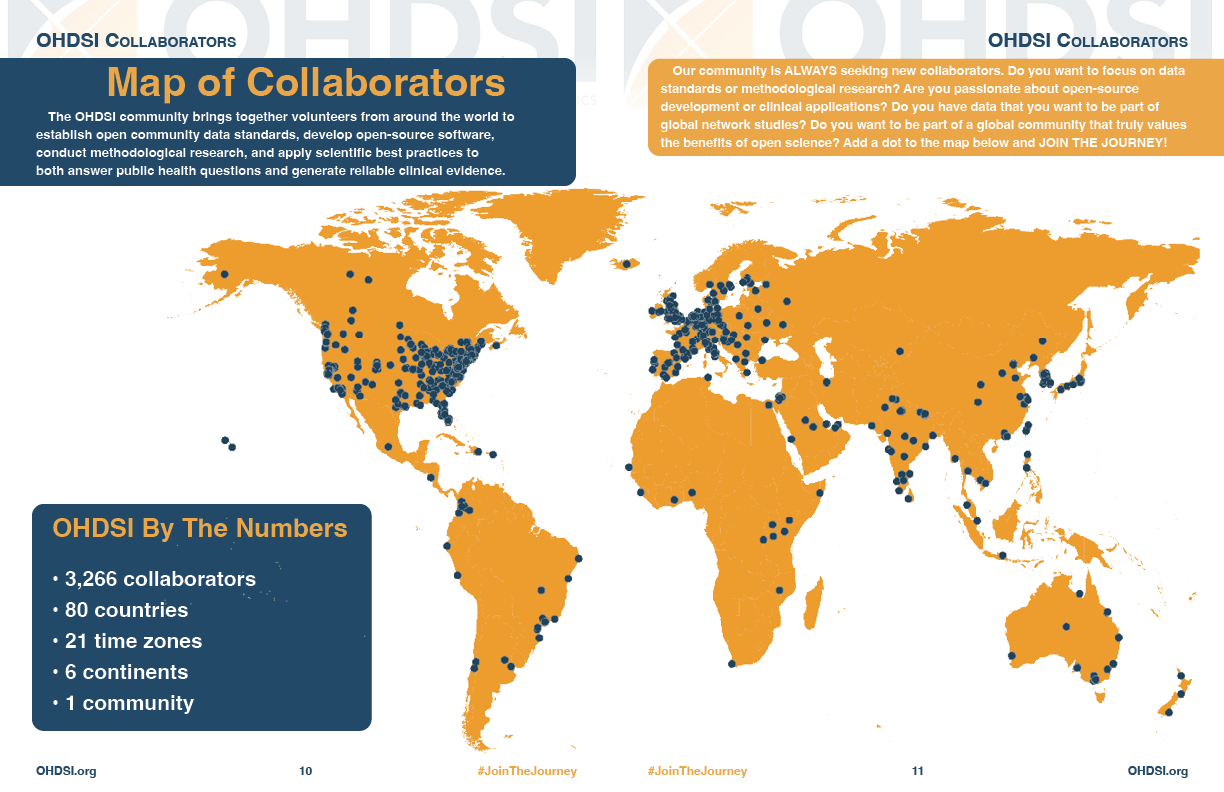
\includegraphics[width=0.80\textwidth]{figures/OHDSIcollaborators.png}
     \caption{Mapa de colaboradores de OHDSI. Extraído de la web oficial \cite{OHDSIwebsite}}
    \label{fig:OHDSIcollaborators}
\end{figure}

Haciendo referencia a la Figura \ref{fig:OHDSIcollaborators} ''Mapa de colaboradores de OHDSI'', la presencia en Europa de la organización es innegable. Desde que inició en 2020 su colaboración con la red europea de datos EHDEN \textit{(European Health Data Evidence)}, está adquiriendo cada vez mayor relevancia. Ejemplo de ello es la celebración este mes de junio en Rotterdam del quinto Symposium Europeo de OHDSI, con el fin de reunir a los expertos y miembros de la comunidad para presentar los grandes proyectos nacionales y europeos que se están realizando en toda europa con las herramientas de la comunidad.

%\begin{figure}[H]
%    \centering
%    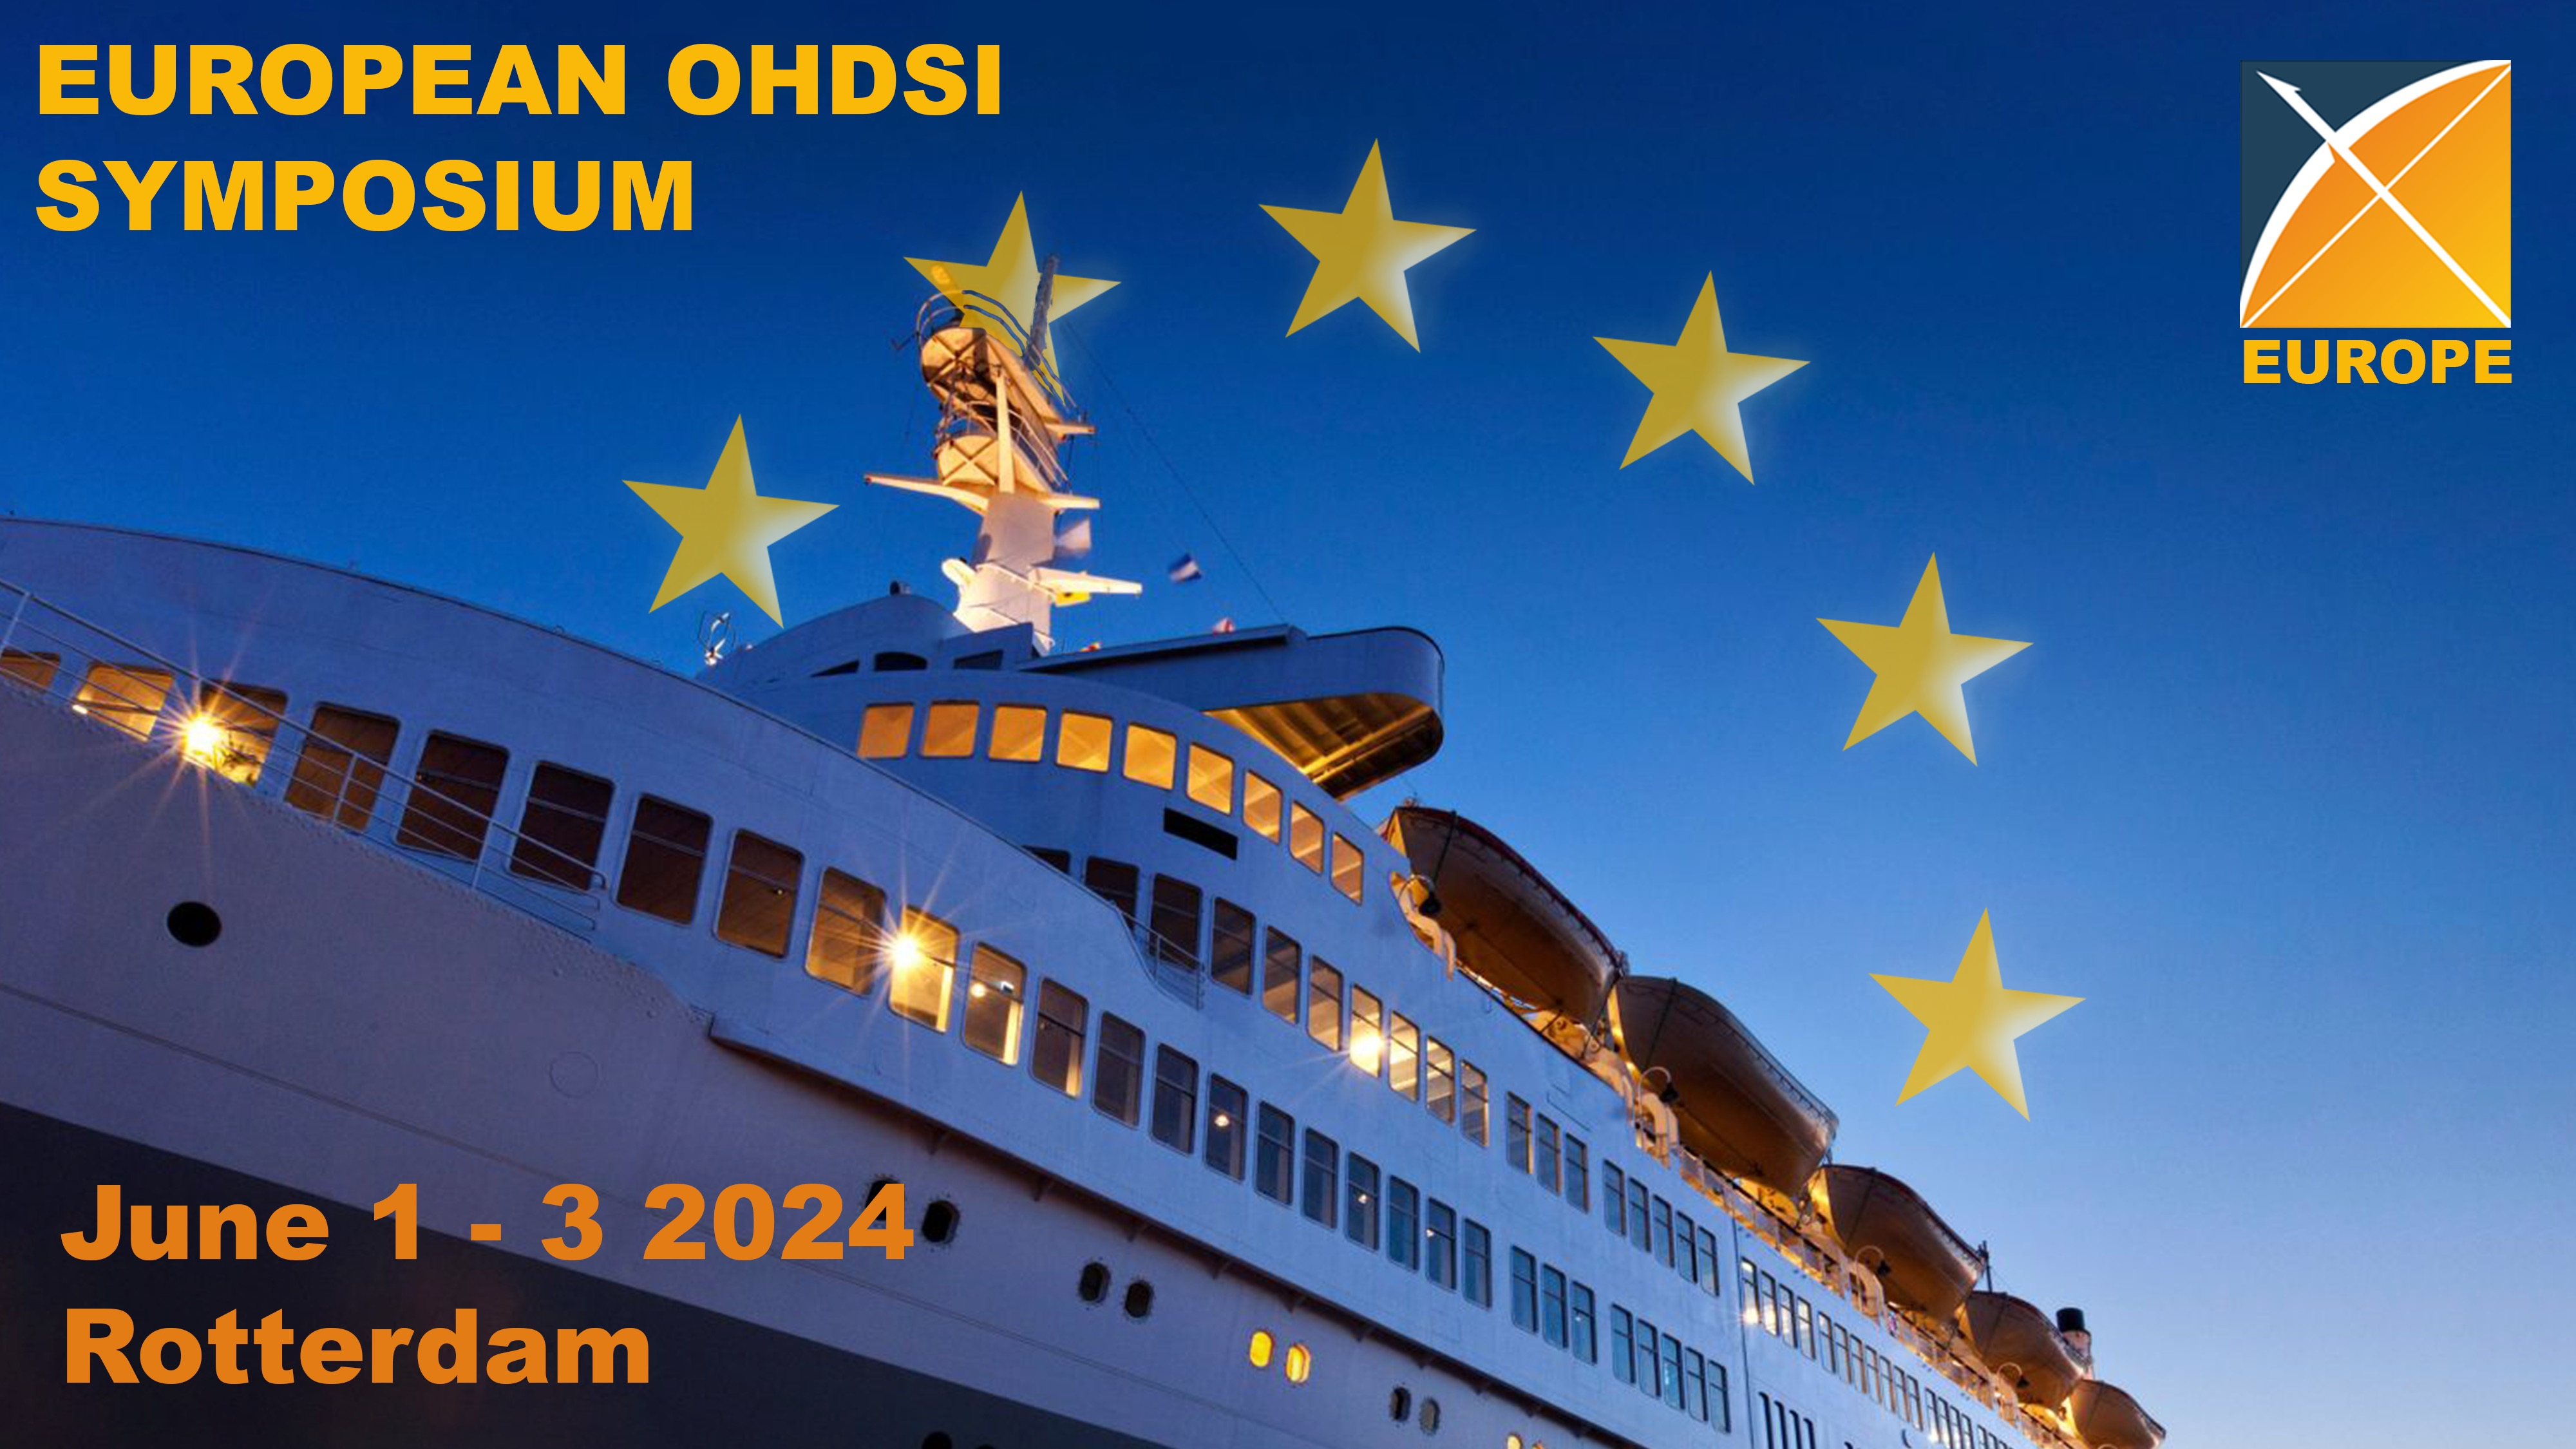
\includegraphics[width=0.70\textwidth]{figures/bannerSymposyum2024.jpg}
%     \caption{Banner del Symposium Europeo 2024. Extraído de la web oficial \cite{OHDSIwebsite}}
%    \label{fig:bannerSymposyum2024}
%\end{figure}

%Por ejemplo, en el Symposium Europeo del pasado año 2023, se presentaron proyectos relativos al almacenamiento de los datos de UCI en Holanda \cite{Jagesar2023The}, la integración del CDM de OMOP con el laboratorio de datos de salud alemám \cite{Finster2023Integrating}, la estandarización de la base de datos nacional francesa SNDS al modelo de OMOP \cite{Collumeau2023Standardization}, la armonización de los HCE hospitalarios en Ruanda al CDM \cite{Halvorsen2023Ruanda} y a la estandarización de los datos del registro europeo de sarcomas a OMOP \cite{vanSwieten2023Standardizing}, entre otros.

\subsection{Características de la organización} \label{subsec:05caracteristicas}

Más allá de los aspectos técnicos de la organización, en esta sección se presentan cuatro características inferidas de la investigación sobre OHDSI, que proveen una visión compresiva de la misma. De esta forma, OHDSI se caracteriza por ser: (i) una comunidad o red colaborativa, (ii) de ciencia abierta, (iii) que promueve la estandarización en salud y (iv) la extracción de evidencia a partir de datos clínicos.

\begin{itemize}

    \item \textbf{Una comunidad o red colaborativa}. La organización es una comunidad abierta a la incorporación de cualquiera que esté comprometido con su misión y valores. Este interés en la incorporación de nuevos colaboradores se muestra constantemente con el eslogan \textit{''Join the Journey''}, en español, ''únete a la aventura''.
    
    La organización distribuye a sus colaboradores en nodos por países y en grupos de trabajo según los diferentes componentes de OHDSI. Por tanto, no se trata de una organización estrictamente burocratizada sino de una unión colaborativa de distintos equipos multidisciplinares que comparten un fin común.

    \item \textbf{Ciencia abierta (\textit{Open science})}. La forma de trabajar de la organización es muy importante, puesto que promueve la colaboración y participación de las organizaciones a través de la ciencia abierta.

    Todos los eventos, publicaciones, herramientas y documentación que elabora OHDSI están disponibles públicamente y de forma gratuita en internet, para que pueda unirse quien quiera (en el caso de los eventos) o consultarse y usarse en cualquier momento (en caso de las herramientas e información). Las dos vías de información por excelencia sobre OHDSI son su página web \cite{OHDSIwebsite} y el \textit{Libro de OHDSI} \cite{OHDSIbook}. 
    
    Otras vías de divulgación son publicaciones científicas \cite{OHDSIpublications}, tutoriales para principiantes, grabaciones de las reuniones semanales de la comunidad o las conferencias anuales a través de su canal de youtube \cite{OHDSIyt}; canales de mensajería abierta como discord \cite{OHDSIdiscordInvitation} o MS Teams \cite{OHDSIofficeForm}, cientos de repositorios de github con información técnica de cada herramienta \cite{OHDSIgithub} y los foros de la comunidad \cite{OHDSIforums} para solventar dudas y preguntas, entre otros.

    Además, en su compromiso con la ciencia abierta, OHDSI asegura la fiabilidad, accesibilidad, interoperabilidad y reproducibilidad de sus estudios a través del cumplimiento de los principios FAIR. Este tema se desarrolla en mayor extensión en la sección 3.7 ''OHDSI and the FAIR Guiding Principles'' del Libro de OHDSI \cite{OHDSIbook}.

    \item \textbf{Promoción de estándares en salud}. OHDSI aboga por estandarizar a un modelo común no solo los modelos de datos sino también la metodología de la investigación médica, con la finalidad de aumentar la interoperabilidad entre los sistemas y organizaciones sanitarias a nivel mundial.
    
    En el Symposium de 2023 se presentó un ejemplo muy intuitivo para divulgar este concepto tan importante: la conexión a la corriente eléctrica a través de una plancha. 
    
    %La conexión de la plancha sería la realización de un estudio sobre unos datos, que serían el enchufe a la corriente eléctrica, siendo el objetivo establecer un enchufe estándar que permita la conexión de la plancha a la corriente eléctrica en cualquier lugar del mundo, es decir, la realización de un estudio siguiendo una misma estructura en cualquier lugar del mundo.

\begin{figure}[H]
    \centering
    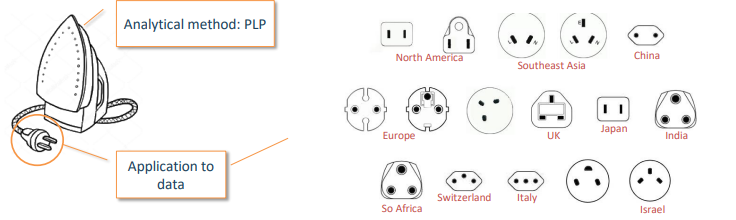
\includegraphics[width=0.60\textwidth]{figures/plancha1.png}
     %\caption{Ejemplo de la plancha con diferentes enchufes. Extraído de la web oficial \cite{OHDSIwebsite}}
    \label{fig:plancha1}
\end{figure}
\begin{figure}[H]
    \centering
    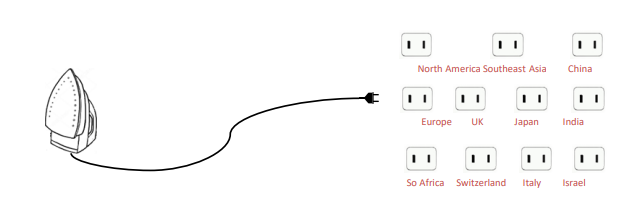
\includegraphics[width=0.70\textwidth]{figures/plancha2.png}
     \caption{Ejemplo de la plancha. Extraído de la web oficial \cite{OHDSIwebsite}}
    \label{fig:plancha2}
\end{figure}

    Como se muestra en la Figura \ref{fig:plancha2} ''Ejemplo de la plancha'', la plancha sería el diseño de un estudio observacional y el enchufe de pared, la base de datos. En el dibujo de arriba se presenta la problemática actual: un mismo estudio no se puede realizar o ''enchufar'' a distintas bases de datos porque no comparten la misma estructura. El objetivo de la organización se muestra abajo: estandarizar las bases de datos con una misma estructura para que un mismo estudio pueda aplicarse a diferentes bases de datos.

    Con este fin OHDSI promueve el uso del Modelo de Datos Común de OMOP (véase en mayor extensión en \ref{subsec:07cdm} ''Modelo de Datos Común'') para estandarizar las bases de datos observacionales. Por otro lado, para conducir los diferentes estudios de forma estandarizada, con el objetivo de fomentar su trazabilidad y reproducibilidad, se ofrecen marcos e instrucciones teóricas sobre cómo conducir los estudios (véase a continuación \ref{sec:05Evidencia} ''¿Cómo generar evidencia?'') y herramientas de análisis estandarizadas, como es el caso de ATLAS y otras herramientas (vease en mayor extensión en \ref{sec:07herramientas} ''Herramientas''). 
    
    Por tanto, \textbf{OHDSI se trata de un ecosistema de herramientas y estándares de salud.} Este ecosistema se describe en mayor detalle en el capítulo \ref{cap:07entorno} ''Entorno de Trabajo''.

    \item \textbf{Extracción de evidencia a partir de datos observacionales}. Es importante destacar que la finalidad de OHDSI no es solo recopilar y almacenar la información clínica de forma estándar, sino también la extracción de información o evidencia de la misma. 
    %La organización identifica la dificultad de extraer información trascendental de los datos clíncos debido a sus distintas morfologías y estructuras en las que son recogidos. 
    %Este es el propósito final y enfrenta muchos desafíos debido a la disparidad de los datos y técnicas de análisis. 
    
    El proceso de extracción de evidencia no es sencillo, como se muestra en la Figura \ref{fig:drawinJourney} ''Dibujo del proceso de extracción de evidencia'', y parte en un extremo de las diferentes bases de datos del mundo real (RWD) hacia la obtención fiable de evidencia del mundo real (RWE). %Por suerte, la organización también proporciona un conjunto de herramientas (véase \ref{sec:05herramientas} ''Herramientas'') para realizar más sencillamente todo el recorrido.

\begin{figure}[H]
    \centering
    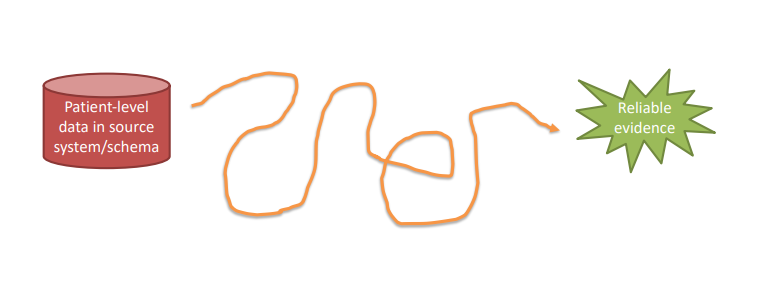
\includegraphics[width=0.80\textwidth]{figures/drawinJourney.png}
     \caption{Dibujo del proceso de extracción de evidencia. Extraído de la web oficial \cite{OHDSIwebsite}}
    \label{fig:drawinJourney}
\end{figure}

    \textbf{La organización se compromete fielmente con este cometido de facilitar la extracción de evidencia a partir de datos observacionales} y para facilitar este proceso ofrece de forma abierta todos los estándares y herramientas mencionados anteriormente. Esta es idea es fundamental en OHDSI y se describe en mayor detalle a continuación, en la sección \ref{sec:05Evidencia} ''¿Cómo generar evidencia?''.

\end{itemize}

%\section{Historia: Observational Medical Outcomes Partnership (OMOP)}

\section{¿Qué es OMOP?} \label{sec:05omop}

Es común encontrar en internet los términos OHDSI y \textbf{OMOP (Observational Medical Outcomes Partnership)}, utilizados de forma casi indistintiva. Si bien es verdad que OMOP se suele asociar mayoritariamente al CDM (\textit{Common Data Model}) también OHDSI mantiene gran relación con este modelo común de datos. Entonces, ¿cuál es la relación entre estas dos entidades? Pues bien, \textbf{la relación que guardan estas dos entidades es filial, OHDSI (2014-Actualidad) es la sucesora de OMOP (2008-2013)}.

OMOP nació en 2008 como una asociación público-privada presidida por la Administración de Alimentos y Medicamentos de EE. UU. y administrada por la Fundación de los Institutos Nacionales de Salud y financiado por un consorcio de compañías farmacéuticas en colaboración con otros investigadores académicos y socios de datos de salud \cite{stang2010advancing}. El propósito inicial de OMOP fue impulsar la ciencia de la vigilancia activa de la seguridad de los productos médicos mediante el análisis de datos observacionales de atención médica \cite{stang2010advancing}. Sin embargo, durante su desarrollo, se enfrentó a los desafíos técnicos de llevar a cabo investigaciones en bases de datos observacionales muy heterogéneas entre sí.

Frente a esta problemática, el resultado fue el desarrollo de un Modelo Común de Datos (CDM) como un mecanismo para estandarizar la estructura, el contenido y la semántica de los datos observacionales %y hacer posible escribir código de análisis estadístico que fuera reutilizable para estudios en distintas fuentes de datos 
\cite{overhage2012validation}. Los experimentos de OMOP demostraron la viabilidad de establecer un CDM que además reuniese diferentes vocabularios estandarizados, reuniendo en un mismo estándar diversos tipos de datos de diferentes entornos de atención y representados por diferentes vocabularios de origen. Esta característica facilitó la colaboración y aumentó el interés entre diferentes instituciones lo que promovió o un enfoque de ciencia abierta \cite{OHDSIbook}. OMOP puso todo su trabajo a disposición del público, incluidos diseños de estudio, estándares de datos, código de análisis y hallazgos empíricos, para mejorar la transparencia y fomentar la confianza en su investigación. 

Al término del proyecto, el Modelo Común de Datos (CDM) de OMOP había evolucionado hasta respaldar un abanico  amplísimo de aplicaciones analíticas de todo el sistema de salud, no solo de la industria farmacéutica. Finalmente, el equipo de investigación acordó que el fin de dicho proyecto debía ser el origen de uno nuevo y a partir de esta idea nació OHDSI \cite{OHDSIbook}.


\section{¿Cómo generar evidencia?} \label{sec:05Evidencia}

La extracción de evidencia a partir de estudios de datos clínicos observacionales es la finalidad fundamental de OHDSI (véase \ref{sec:05OHDSI} ''¿Qué es OHDSI?''). 

%Este proceso generalmente es bastante complejo, debido a la disparidad de estructuras en la que se recopilan los datos de salud y la disparidad de metodologías en las que se conducen los estudios, lo que imposibilita y/o dificulta la interoperabilidad entre los sistemas de información sanitaria (véase \ref{sec:01Contexto} ''Contexto'').

%Frente a ello, OHDSI propone un marco estándar para generar evidencia basada en la estandarización de los datos clínicos al Modelo de Datos Común de OMOP y la definición de tres tipos de estudios observacionales o ''\textit{casos de uso}''. Además proporciona un conjunto de herramientas estandarizadas con las que realizar todas las tareas implicadas en el proceso con el fin de facilitar la generación de evidencia interoperable entre los distintos nodos y organizaciones de su comunidad.

Por ello, no es casualidad que la invitación que hace OHDSI a sus colaboradores lleve el slogan \textit{''Join the Journey''} (véase anteriormente \ref{subsec:05caracteristicas} ''Características de la organización''), sino que es un guiño al propósito al que se unen: al camino desde los datos hacia la evidencia o, en ingles, \textit{\textbf{"The Journey from data to evidence"}}.  

%A continuación, en las secciones \ref{subsec:05journey}, \ref{subsec:05invest}, \ref{subsec:05vias} se presentan los conceptos fundamentales para comprender este proceso desde el punto de vista de la organización.

%\subsection{El camino desde los datos hacia la evidencia} \label{subsec:05journey}

\begin{figure}[H]
    \centering
    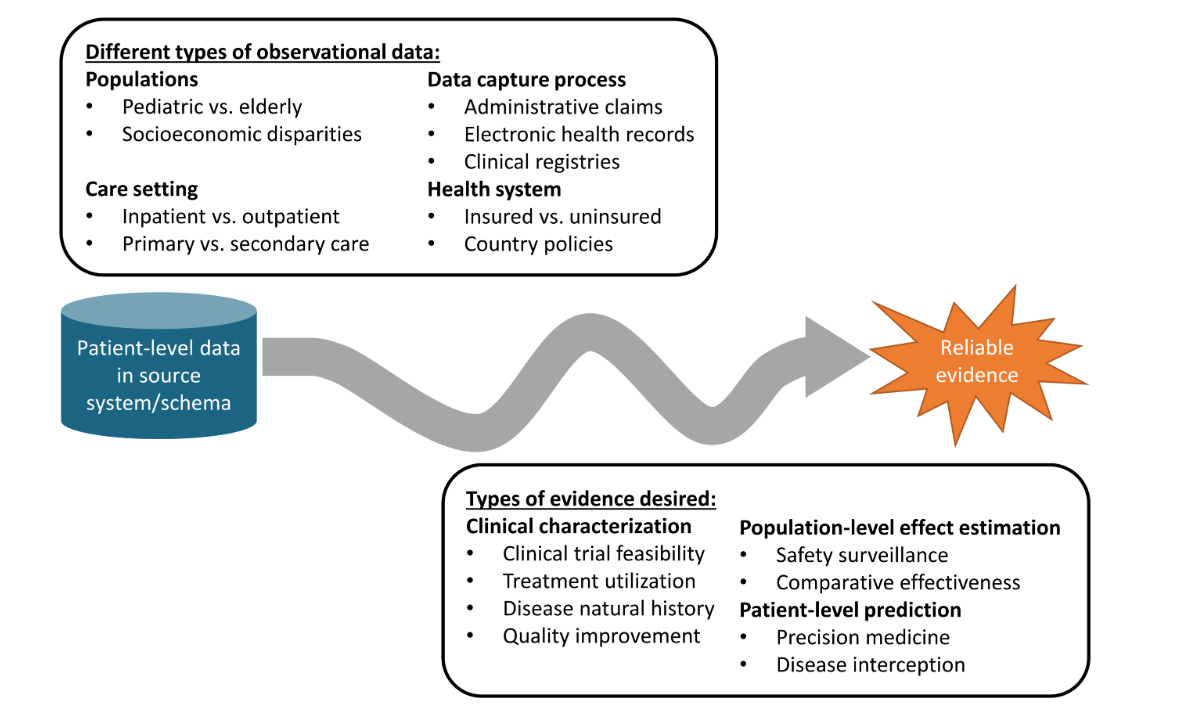
\includegraphics[width=0.80\textwidth]{figures/journeyDataToEvidence.png}
     \caption{\textit{The Journey from Data to Evidence}. Extraído del Libro de OHDSI \cite{OHDSIbook}}
    \label{fig:journeyDataToEvidence}
\end{figure}

La Figura \ref{fig:journeyDataToEvidence} ''The Journey from Data to Evidence'' complementa a la anterior Figura \ref{fig:drawinJourney} ''Dibujo del proceso de extracción de evidencia'' añadiendo mayor información en los extremos del recorrido, definiendo cuatro tipos distintos de bases de datos observacionales y tres tipos de evidencia que se quiere generar: la caracterización clínica \textit{(clinical characterization)}, la estimación de efectos a nivel de población (\textit{Population-level effect estimation)} y la predicción a nivel de paciente \textit{(Patient-level prediciton)}. Estos tres ''casos de uso'' se presentan en mayor profundidad a continuación en  \ref{subsec:05casosUso} ''Casos de uso para la investigación''.

%Esta definición de tres \textit{''casos de uso''} en la investigación se detalla en mayor profundidad en

Con ello la organización define un marco para llevar a cabo \textbf{estudios observacionales o fenotípicos} sobre datos. Un estudio observacional es una investigación que observa y recopila información sobre individuos o fenómenos sin intervenir en ellos.
En el caso del estudio sobre datos, en vez de realizar seguimientos de estudios clínicos en vivo, se simulan estos estudios sobre una base de datos. Cuando la evidencia se extrae sobre datos del mundo real (\textit{RWD}), se denomina evidencia del mundo real (\textit{Real World Evidence, RWE}). 

En OHDSI la conducción de estos estudios observacionales se realiza mediante el diseño y estudio de cohortes en la base de datos. Concretamente, se trata de \textbf{estudios de cohortes retrospectivos} porque los sujetos se estudian después de haberse producido la enfermedad, utilizando para ello bases de datos que tengan registrada información histórica de la enfermedad y de los factores de riesgo que hayan podido provocar dicha enfermedad.

A continuación en \ref{subsec:05cohortes} ''Cohortes'' se presenta este concepto en profundidad.

%Frente a la disparidad de los datos y la finalidad con la que son recogidos, OHDSI presenta el Modelo de Datos Común (véase la subsección \ref{subsec:05cdm} ''Modelo de Datos Común'') y para la extracción de evidencia, la investigación metodológica mediante tres casos de uso fundamentales: la caracterización clínica de una cohorte, la estimación a nivel de población y la predicción a nivel de paciente (véase subsección \ref{subsec:05investMetodolog} ''Investigación metodológica'').

%De esta forma, OHDSI promueve una vía para generar evidencia interoperable entre las distintas organizaciones que interactúan a través de su red mundial, dicho de otra forma, da soporte para que diferentes estudios se realicen siguiendo una misma metodología que facilite su comprensión y reproducibilidad de forma global, como se sugería en el ejemplo de la plancha (véase anteriormente \ref{subsec:05caracteristicas} ''Características de la organización'').

\subsection{Cohortes} \label{subsec:05cohortes}

%Además, una característica fundamental de las investigaciones que se llevan acabo en OHDSI es que giran entorno al paciente, que es además el núcleo central del Modelo de Datos Común de OMOP. 

El componente central de cualquier investigación en OHDSI es el paciente, del que se recopilan las denominadas ''historias del paciente''. \textbf{Para cada evento clínico que sucede se recoge una historia del paciente o \textit{Patient Journey}}. %Es importante no confundir este concepto con la Historia Clínica Electrónica de un paciente (HCE) que recoge una ficha con todos los eventos que han le sucedido a lo largo de su vida. 
Las investigaciones observacionales se diseñan para extraer información sobre la recopilación de todas las historias de paciente registradas en la base de datos.

La historia del paciente,  como se muestra en la Figura \ref{fig:patientJourney} ''The patient journey'', es por tanto, una ventana temporal que recoge un evento clínico que le sucede a un paciente en un período de tiempo concreto. El evento se describe mediante tres períodos de tiempo: la enfermedad (rojo), el tratamiento (naranja) y el efecto (verde); y a partir de distintas características como enfermedades (\textit{conditions}), medicamentos (\textit{drugs}), procedimientos (\textit{procedures}) y pruebas (\textit{measurements}).

\begin{figure}[H]
    \centering
    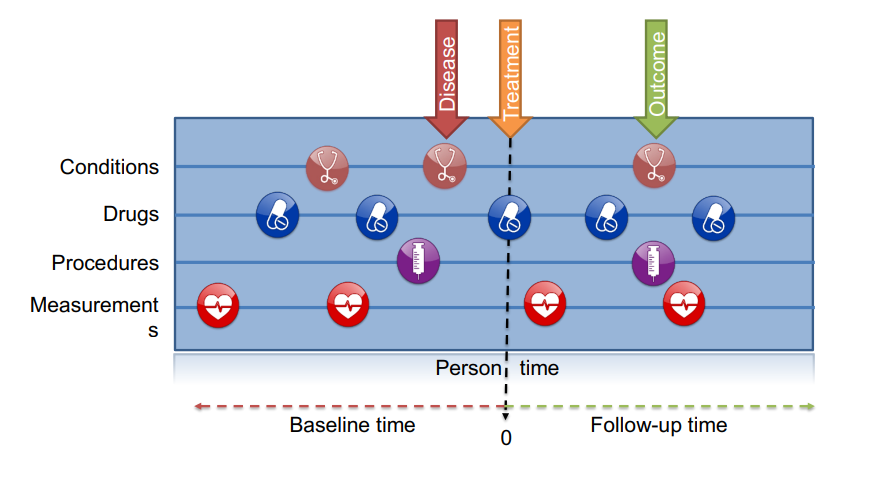
\includegraphics[width=0.80\textwidth]{figures/patientJourney.png}
     \caption{\textit{The patient journey}. Extraído de la página web oficial \cite{OHDSIbook}}
    \label{fig:patientJourney}
\end{figure}

Los pacientes se pueden agrupar en \textbf{cohortes} cuando comparten historias y características similares, al igual que a la hora de realizar un estudio clínico en vivo. Las diferentes  prácticas para los análisis de cohortes darán lugar a los diferentes tipos de evidencia deseada (caracterización, estimación a nivel de población, predicción a nivel de paciente). \textbf{Por tanto, el componente central para generar evidencia en OHDSI es el diseño de cohortes.}

%\begin{figure}[H]
%\centering
%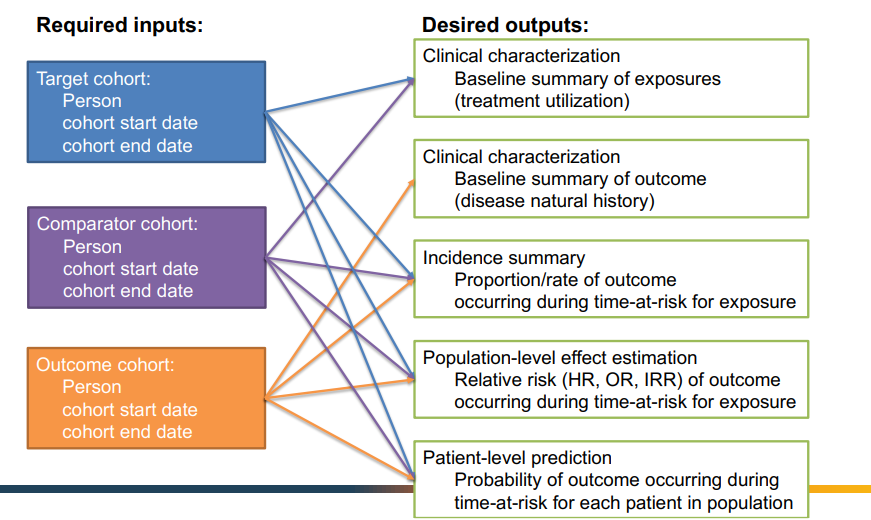
\includegraphics[width=0.70\textwidth]{figures/studyIO.png}
%     \caption{La definición de cohortes es el componente esencial para la generación de evidencia. Extraído del Tutorial2022 publicado en la web oficial \cite{OHDSIwebsite}}
%    \label{fig:studyIO}
%\end{figure}

\textbf{En OHDSI una cohorte es un ''conjunto de personas que satisface uno o más criterios de inclusión durante un periodo de tiempo concreto''} \cite{OHDSIbook}. Definir correctamente la cohorte es fundamental a la hora de realizar cualquier estudio fenotípico en OHDSI y es crucial para realizar un buen análisis \cite{hripcsak2018high}. A continuación se presenta esquemáticamente la estructura fundamental de una cohorte, denominada en OHDSI ''anatomía de una cohorte''.

\begin{figure}[H]
\centering
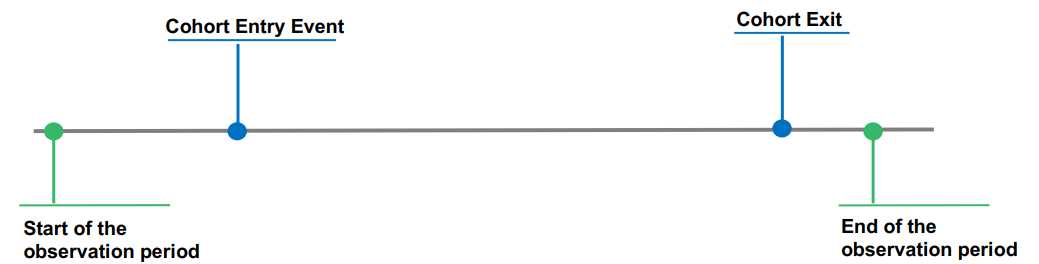
\includegraphics[width=0.90\textwidth]{figures/cohortAnatomy.png}
     \caption{''Anatomía de una cohorte''. Extraída del Tutorial 2022 publicado en la web oficial \cite{OHDSIwebsite}}
    \label{fig:cohortAnatomy}
\end{figure}

La investigación observacional comprende un intervalo temporal delimitado por el comienzo del período de  observación (\textit{Start of the observation period}, en verde) y el fin del periodo de observación (\textit{End of the observation period}, en verde).

Dentro del periodo de observación, la cohorte se define con un  evento de entrada a la cohorte (\textit{Cohort Entry Even}t, en azul) y un evento de salida de la cohorte (\textit{Cohort Exit}, en azul). 

\begin{itemize}

    \item \textbf{Evento de entrada.} Define el evento que cualifica al paciente para entrar a la cohorte. El conjunto de pacientes que satisfacen el evento de entrada conforman la cohorte inicial. 

    \item \textbf{Evento de salida.} Define el evento de salida de la cohorte, cuando el paciente ya no es elegible para formar parte de la cohorte.

\end{itemize}

Adicionalmente, la cohorte puede definirse más específicamente mediante una serie de \textbf{criterios de inclusión}. La cohorte que satisface todos los criterios de inclusión se denomina cohorte cualificada.

\subsection{Casos de uso para la investigación} \label{subsec:05casosUso}

Con el fin de estandarizar y proveer un marco metodológico en el camino hacia la generación de evidencia, OHDSI define tres casos de usos que establecen los diferentes tipos de estudio que se pueden realizar: (i) la caracterización, (ii) la estimación a nivel de población (iii) la predicción a nivel de paciente.

\begin{figure}[H]
\centering
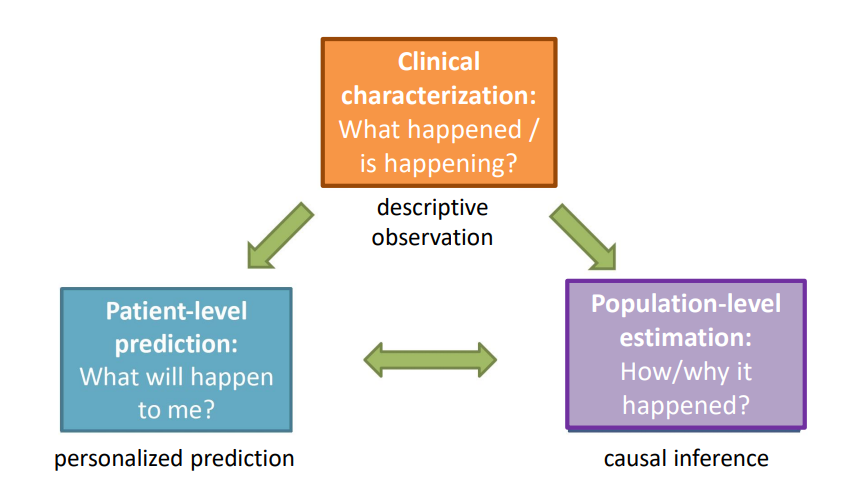
\includegraphics[width=0.80\textwidth]{figures/useCases.png}
     \caption{Esquema simplificado de los casos de uso para la investigación en OHDSI. Extraído del Symposium 2023, publicado en la web oficial \cite{OHDSIwebsite}}
    \label{fig:useCases}
\end{figure}

%Estos tres casos de uso se presentan generalmente en los \textit{Symposium} y \textit{Workshops}, para dar a conocer a la comunidad el esquema propio de investigación de OHDSI. Además el Libro de OHDSI \cite{OHDSIbook} los presenta de forma general en el capítulo 7 y de forma específica para cada caso de uso en los capítulos 11, 12 y 13, respectivamente. 

Anteriormente se definieron las historias de paciente como marco fundamental de la investigación (véase \ref{subsec:05cohortes} ''Cohortes''). Cada caso de uso extrae un tipo de evidencia distinto a partir de la historia del paciente, tal y como se muestra a continuación en la Figura \ref{fig:useCasesJourney} ''Esquema de los casos de uso encuadrado en la historia del paciente''.


\begin{figure}[H]
\centering
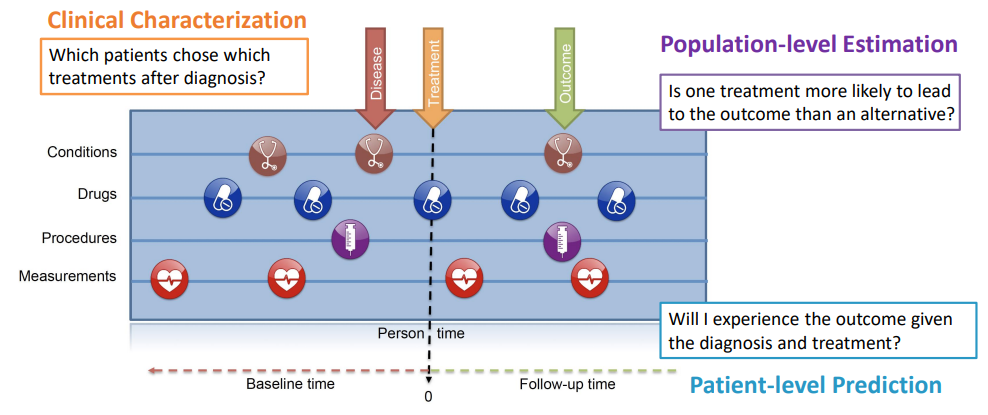
\includegraphics[width=1\textwidth]{figures/useCasesJourney.png}
     \caption{Esquema de los casos de uso encuadrado en la historia del paciente. Extraído del Symposium 2023 publicado en la web oficial \cite{OHDSIwebsite}}
    \label{fig:useCasesJourney}
\end{figure}

La historia del paciente definirá la pertenencia o no del paciente a una cohorte y sobre esa cohorte se realizarán los distintos tipos de estudio. \textbf{El conjunto de estos tres casos de uso y la definición de cohortes conforma la metodología OHDSI para la generación de evidencia}. A continuación se describe brevemente cada uno de los casos de uso. 

\subsubsection{Caracterización}

La caracterización busca la caracterización a nivel estadístico de una cohorte o una base de datos. Es una mera descripción estadística de los datos, sin realizar inferencias, predicciones o análisis más complejos, simplemente observando la base de datos.

Responde a la pregunta de investigación: \textbf{¿Qué les ha pasado?}

Obtiene como resultados: recuentos y porcentajes, medias, estadísticas descriptivas, ratios de incidencia...

\subsubsection{Estimación a nivel de población}

La estimación a nivel de población busca realizar inferencias causales sobre los efectos de las intervenciones sanitarias en la población. Se pretende entender los efectos causales para comprender las consecuencias de las acciones.

Responde a la pregunta de investigación: \textbf{¿Cuáles son los efectos causales?}

Obtiene como resultados: riesgos relativos, efectos causales, correlación entre variables, comparaciones de efectividad, asociaciones…

\subsubsection{Predicción a nivel de paciente}

La predicción a nivel de paciente busca, en base a los datos obtenidos de los conjuntos de pacientes en la base de datos, realizar predicciones concretas para individuos concreto.

Responde a la pregunta: \textbf{¿Qué me pasará a mi como paciente?}

Obtiene como resultados: probabilidades para un individuo, fenotipos probables, grupos de riesgo… 


\subsection{Vías de implementación del análisis} \label{subsec:05vias}

Para realizar un análisis, OHDSI distingue tres vías alternativas para generar la evidencia a partir de la base de datos estandarizada al OMOP CDM. Estas tres alternativas se muestran a continuación en la Figura \ref{fig:analysisImplementations} ''Tres vías para la implementación de un análisis observacional'', extraída del capítulo 8 del Libro de OHDSI.

\begin{figure}[H]
    \centering
    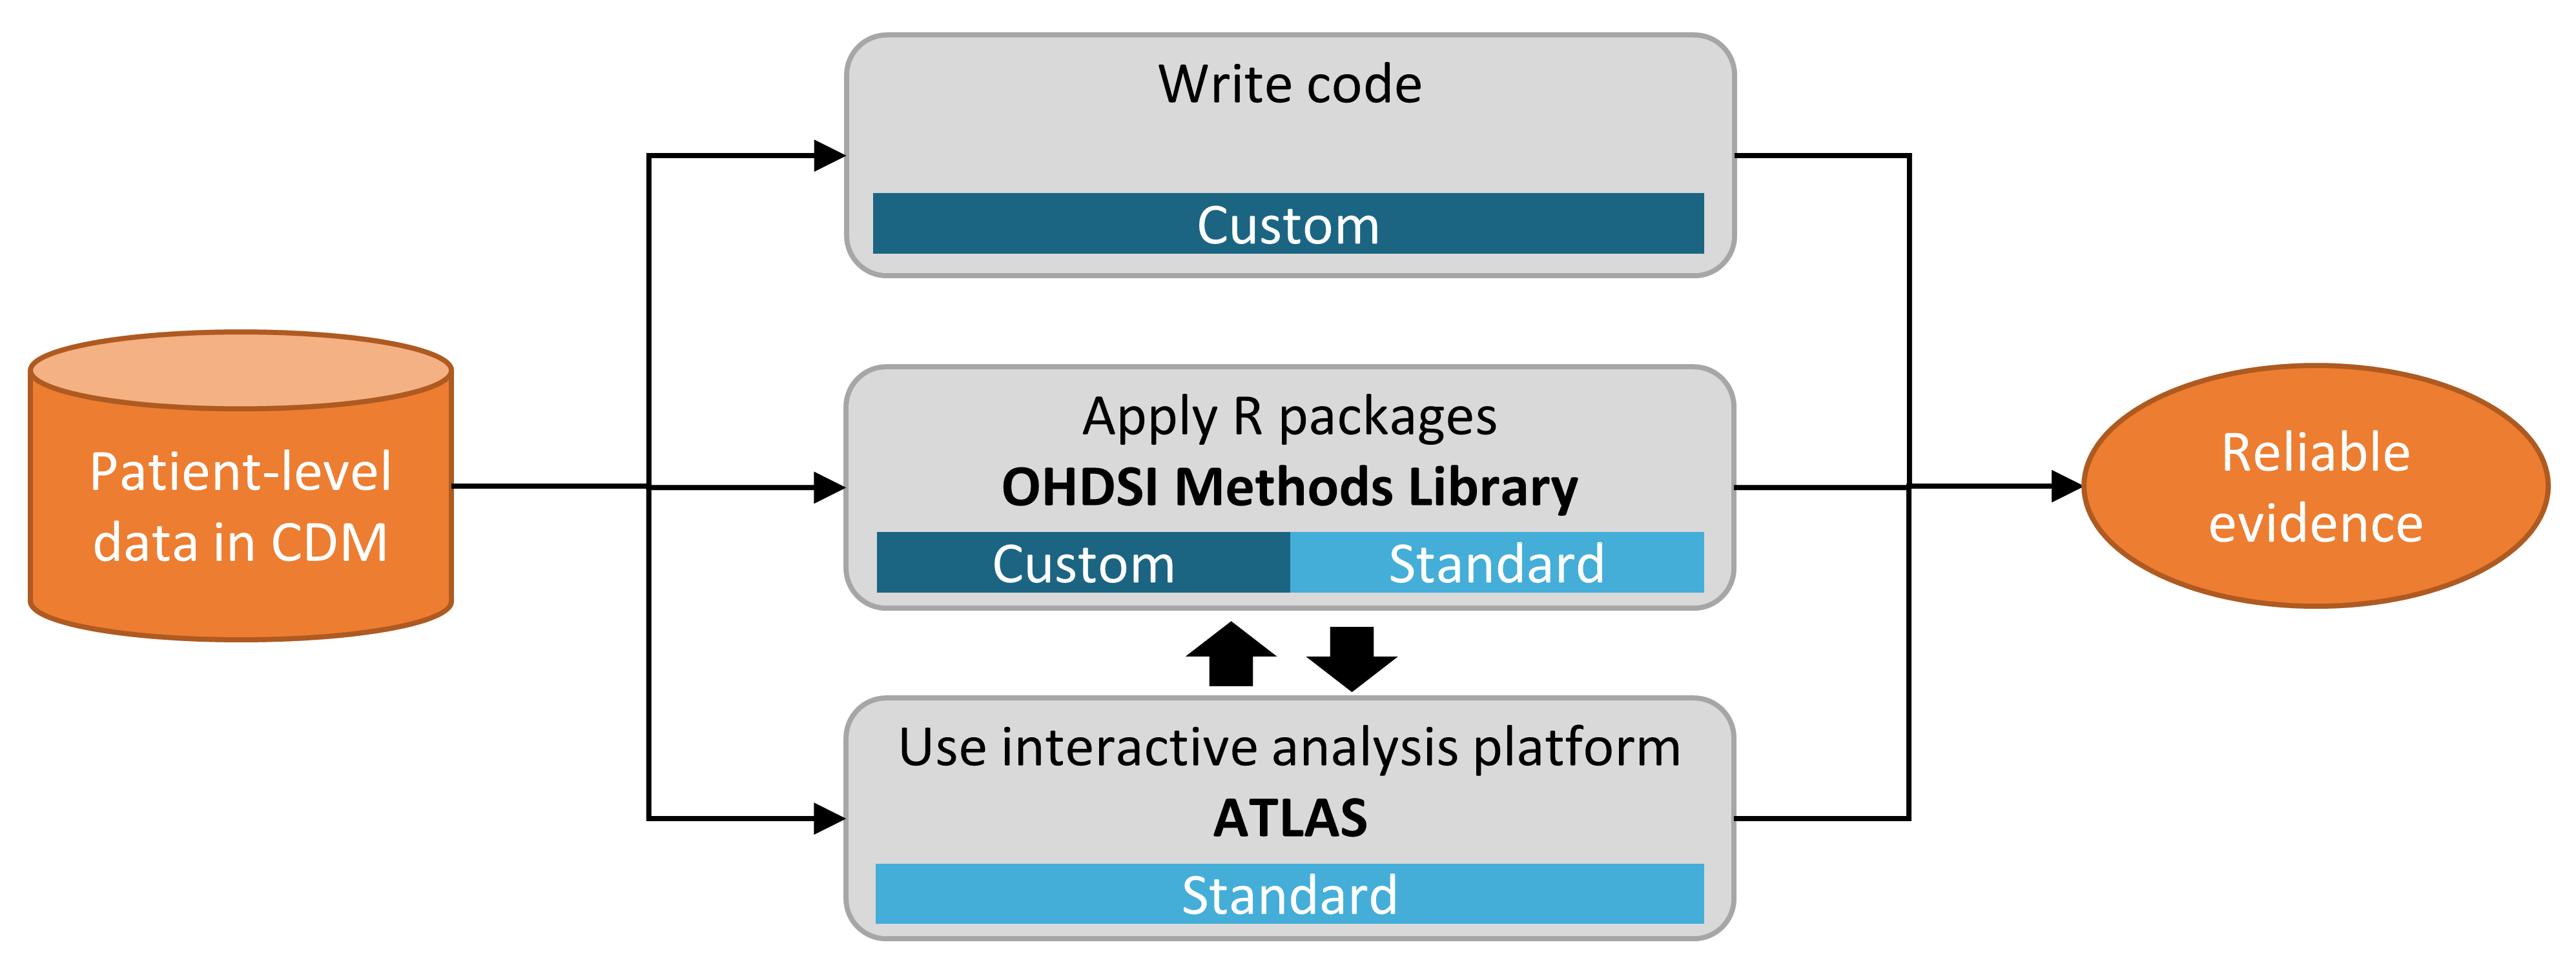
\includegraphics[width=0.80\textwidth]{figures/analysisImplementations.png}
     \caption{Tres vías para la implementación de un análisis observacional. Extraído del Libro de OHDSI \cite{OHDSIbook}}
    \label{fig:analysisImplementations}
\end{figure}

Cada vía se evalúa en cuanto a lo personalizada (\textit{custom}) o estandarizada (\textit{standard}) que es. A estas alturas se debe conocer que la vía más recomendada para implementar el análisis será la más estandarizada, es decir, la tercera vía.

La problemática que presentan la primera y la segunda vía consiste en ser en mayor o menor medida vías customizada, lo que genera problemas de interoperabilidad y reproducibilidad de los estudios. Si bien la primera vía consiste en la programación directa de código para realizar las consultas  (no hay ningún tipo de estandarización, distintos lenguajes de programación, funciones personalizadas) al menos la segunda vía hace uso de librerías estándares en R que OHDSI ofrece (\textit{OHDSI Methods Library}) pero, aunque se use el mismo lenguage de programación y funciones, los scripts pueden ser tan distintos que aún dificulten la interoperabilidad.

Por tanto, la tercera vía se presenta como la alternativa óptima por ser la más estandarizada y es la que empleará el TFG en el estudio práctico. Esto es, usar la herramienta interactiva \textit{low-code} de análisis de datos que ofrece OHDSI, denominada \textbf{ATLAS}, sin necesidad de programar directamente código.

\section{Conclusiones} \label{sec:05conclusion}

En este capítulo se recogen las características fundamentales de OHDSI con el fin de comprender la relevancia de la organización en el panorama sanitario, como sucesora de OMOP y gran candidata para subsanar las dificultades en términos de interoperabilidad y estandarización de la investigación observacional.

Además se explora en mayor profundidad la metodología que promueve la organización en cuanto a la generación de evidencia clínica, a partir del concepto de cohorte y los estudios de caracterización, estimación a nivel de población y estimación a nivel de paciente.
    \chapter{Documento de Requisitos}\label{cap:requisitos}

\section{Introducción}


%R.I%%%%%%%%%%%%%%%%%%%%%%%%%%%%%%%%%%%%%%%%%%%%%%%%%%%%%%%%%%%%%%%%%%%%%
%\section{Requisitos de Información}


%R.F%%%%%%%%%%%%%%%%%%%%%%%%%%%%%%%%%%%%%%%%%%%%%%%%%%%%%%%%%%%%%%%%%%%%%
\section{Requisitos Funcionales}

- RF00: Cargar datasets //De hecho este aún no sabemos como hacerlo. Estamos trabajando con datasets que ya vienen cargados

- RF01: Obtener un reporte del data set (Data source)

- RF02 : Definir un conjunto de conceptos del Vocabulario (Concept set)

- RF03: Configurar la muestra de trabajo (cohort definition)

- RF04: Caracterizar el cohort (characterization - primer gran bloque de metodología de OHDSI)

- RF05: Definir una etsimacion a nivel de poblacion (estimation - segundo gran bloque de metodologia de OHDSI)

- RF06: Hacer una prediccion a nivel de paciente (prediction - tercer gran bloque de metodologia de OHDSI)



Más cosas que se pueden hacer y no definimos la otra vez:

- Obtener un reporte de la ruta del cohorte (cohort pathway)

- Analizar los ratios de incidencia de un outcome (INcidence rate)

- Obteenr un reporte de los datos para un paciente concreto (profile)

\subsection{Diagramas de casos de uso}


\subsection{Descripción del requisito}


%\subsection{Diagramas de casos de uso}
%\subsection{¿¿¿¿¿Descripción del requisito funcional????}


%\section{Modelo conceptual}%%%%%%%%%%%%%%%%%%%%%%%%%%%%%%%%%%%%%%%%%%%%%%

%\section{Mockups}%%%%%%%%%%%%%%%%%%%%%%%%%%%%%%%%%%%%%%%%%%%%%%%%%%%%%%%%

%R.N.F%%%%%%%%%%%%%%%%%%%%%%%%%%%%%%%%%%%%%%%%%%%%%%%%%%%%%%%%%%%%%%%%%%%%
\section{Requisitos no Funcionales}





\section{Conclusiones}
En este capítulo concluimos que...

    \chapter{Entorno de Trabajo}\label{cap:07entorno}
Este capítulo se divide en cinco secciones \ref{sec:07intro} Introducción, \ref{sec:07estandares} Estándares de OHDSI, \ref{sec:07herramientas} Herramientas de OHDSI, \ref{sec:07programas} Programas informáticos empleados y \ref{sec:07conclusiones} Conclusiones.

\section{Introducción}\label{sec:07intro}

En este capítulo se presenta el entorno de trabajo utilizado durante el desarrollo del proyecto. Consiste principalmente en la utilización de los estándares y herramientas que provee OHDSI para conducir estudios observacionales.

\textbf{No se puede entender la herramienta ATLAS sin entender el ecosistema de herramientas y estándares OHDSI que la acompañan}.

Por tanto, en la sección \ref{sec:07estandares} ''Estándares de OHDSI'' se presentan los dos estándares fundamentales: el Modelo de Datos Común de OMOP y el Vocabulario.

En la sección \ref{sec:07herramientas} ''Herramientas de OHDSI'' se presenta el conjunto de herramientas que ofrece la organización, prestando especial atención a la herramienta ATLAS.

Por último, en la sección \ref{sec:07programas} ''Programas informáticos empleados'' se presentan los programas informáticos utilizados para desplegar el entorno de trabajo del proyecto.


\section{Estándares de OHDSI}\label{sec:07estandares}

%\subsection{Estandarización de los datos} \label{subsec:05estandarDatos}

En términos de estandarización, OHDSI realiza una labor muy importante para paliar las dificultades de la investigación con datos de salud a causa de la heterogeneidad de los datos y estudios. Debido a la amplia colaboración internacional de la organización se recocone la necesidad de estándares que permitan el intercambio de información sin pérdida entre los distintos sistemas de información de los miembros de la comunidad.

OHDSI ofrece dos estándares: el Modelo de Datos Común de OMOP y el Vocabulario. A continuación se describe cada uno de ellos en mayor detalle.

%La estandarización de la investigación en OHDSI se realiza en dos planos: a nivel de datos y a nivel de investigación. La estandarización a nivel de datos se realiza a través del uso del Modelo de Datos Común y el Vocabulario y la estandarización a nivel de investigación mediante la ''investigación metodológica''. A continuación se describe en una subsección cada uno de estos estándares.

\subsection{Modelo de Datos Común de OMOP} \label{subsec:07cdm}

El Modelo de Datos Común o \textit{Common Data Model (CDM)} de OMOP es ''un estándar de datos comunitario abierto, diseñado para estandarizar la estructura y el contenido de los datos de observación y permitir análisis eficientes que puedan producir evidencia confiable'' \parencite{gitPagesCMD}, en definitiva, es un modelo semántico estándar para estructurar los datos de salud. La información más relevante y actualizada sobre el CDM se encuentra en su página de github \parencite{gitPagesCMD} y en el capitulo 4 del Libro de OHDSI \parencite{OHDSIbook}.

\subsubsection{Características}

El modelo de datos de OMOP presenta características importantísimas para hacer frente a las necesidades del panorama socio-sanitario actual presentado en la sección \ref{sec:01Contexto} ''Marco Contextual''. A continuación se presentan las características más relevantes del modelo (extraídas de la sección  4.1 del Libro de OHDSI \parencite{OHDSIbook}), según las necesidades identificadas previamente.

\begin{itemize}
    \item \textbf{Estructura diseñada para la investigación}. 
    El modelo presenta una estructura única y óptima para un propósito concreto: el de facilitar la realización de estudios observacionales. Por tanto reduce notoriamente los desafíos relativos a las diferentes estructuras y propósitos con los que se recogen los datos clínicos.
    \item \textbf{Modelo centrado en el paciente}. Es un modelo centrado en el paciente (alineado con la misma característica de la Sanidad 4.0). Estructuralmente esto significa que todos los eventos y tablas están relacionados con la tabla central del paciente, denominada \textit{Person}. 
    \item \textbf{Protección y privacidad}. El modelo limita el acceso a la información personal de los pacientes, evitando en la medida de lo posible el acceso a información personal sensible como nombres o apellidos, para fomentar la protección y privacidad de los datos. Mayor información sobre las técnicas empleadas para ello se encuentran en el apartado \textit{Privacidad del paciente y OMOP} de la página de github \parencite{gitPagesCMD}.
    \item \textbf{Reutilización de estándares}. Un aspecto importantísimo es que el modelo propone su propio estándar pero sin olvidar los estándares globalmente utilizados, de manera que integra y reutiliza los conceptos provenientes de estándares ya existentes (ej. SNOMED, LOINC...) referenciándolos en su propio Modelo de Datos Común. El conjunto de todos los estándares conforma el Vocabulario.
    \item \textbf{Neutralidad tecnológica}. El modelo no requiere una tecnología específica sino que puede estructurarse en cualquier base de datos relacional (ej. Oracle, SQL Server...), ajustándose a los requisitos tecnológicos necesarios de cada organización.
    
\end{itemize}

\subsubsection{Modelo de Datos Lógico}

Actualmente el CDM ha lanzado ya su sexta versión, sin embargo, esta aún no está soportada por todas las herramientas de la comunidad, por lo que se sigue sugiriendo el uso del CDM v5.4 o 5.3 indistintivamente, que son las últimas versiones completamente funcionales. 

A la hora de realizar un estudio en ATLAS o cualquier otra herramienta del ecosistema OHDSI la base de datos estará necesariamente estandarizada a este modelo por lo que es importante conocer su estructura fundamental. A continuación, en la Figura \ref{fig:cdm54} ''Estructura del CDM v5.4'' se presenta la estructura lógica de este modelo y en la Figura \ref{fig:cdm_ER} ''Modelo Entidad-Relación del CDM v5.4'', la estructura del modelo Entidad-Relación. Adicionalmente existe una página web que proporciona un modelo interactivo para facilitar su estudio \parencite{CDMinteractive}.

Aunque el modelo de datos común de OMOP es muy complejo, incluso existen grupos de trabajo de la comunidad (\textit{workshops}) especializados sólo en este ámbito, en esta subsección del trabajo tan solo se van a presentar los conceptos considerados estrictamente necesarios para la comprensión del contenido del mismo.

\begin{figure}[H]
    \centering
    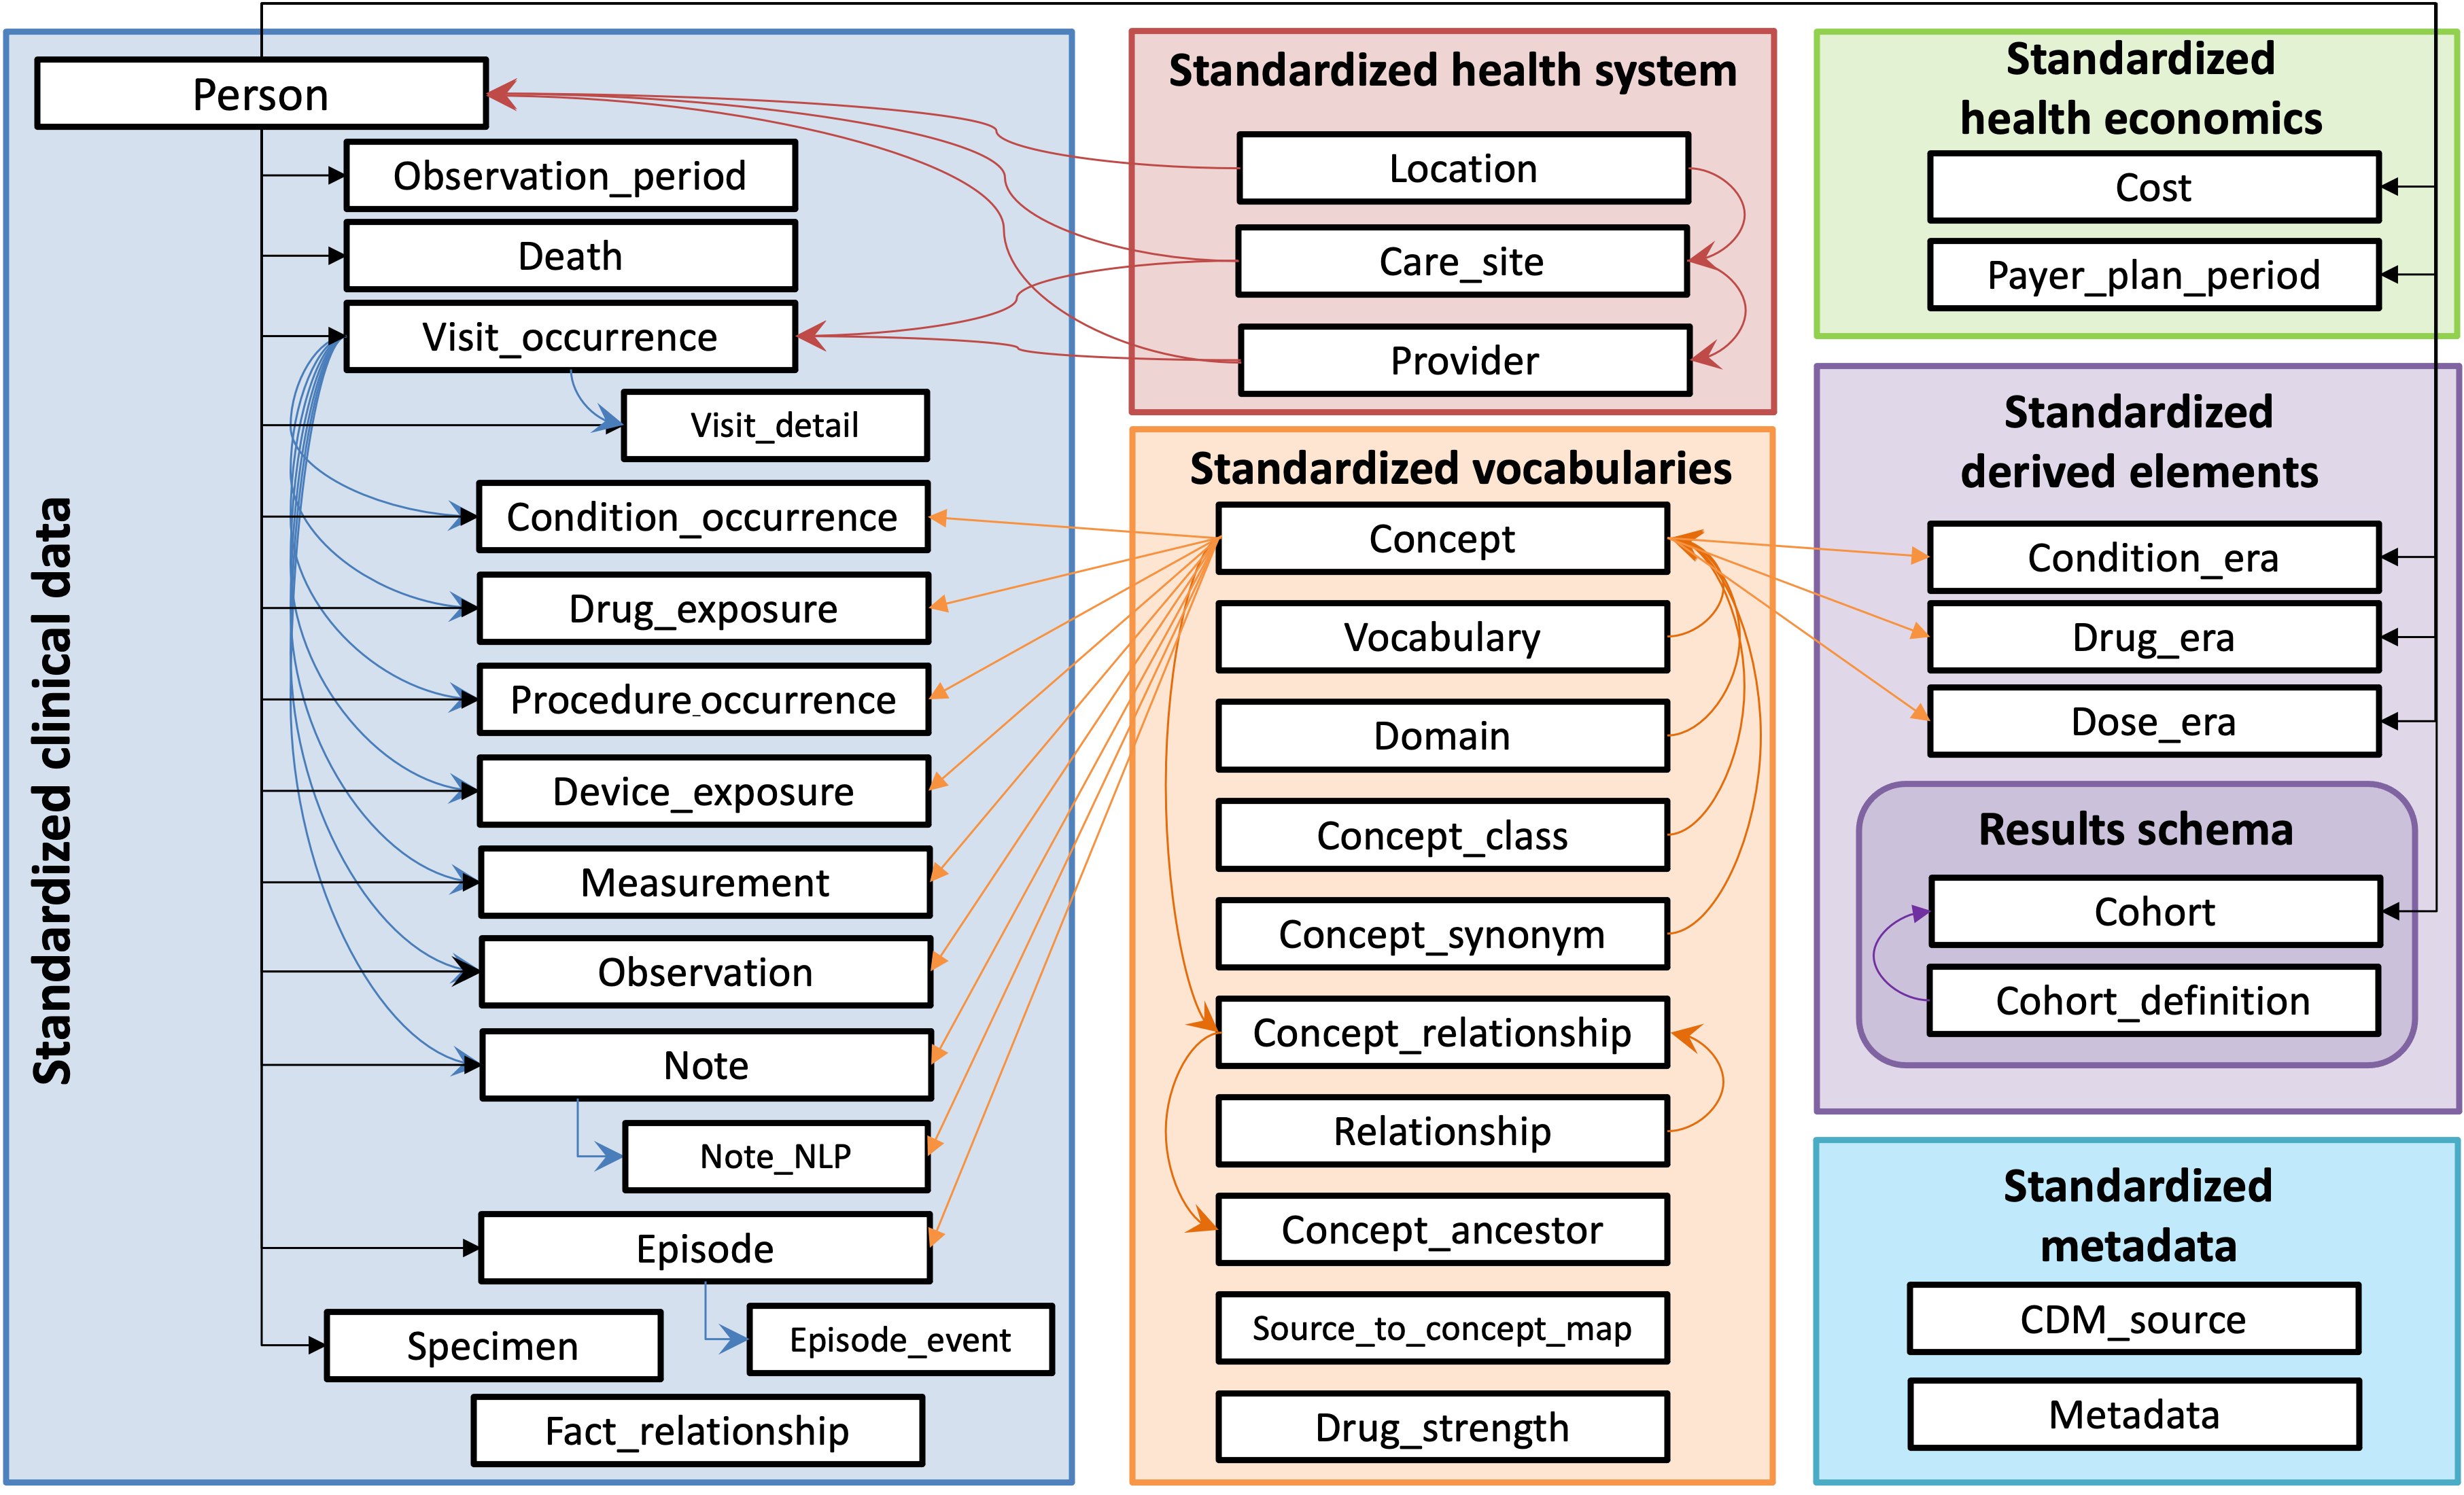
\includegraphics[width=1\textwidth]{figures/cdm54.png}
     \caption{Estructura del CDM v5.4. Extraída de la página de github del CDM \parencite{gitPagesCMD}}
    \label{fig:cdm54}
\end{figure}

\begin{figure}[H]
    \centering
    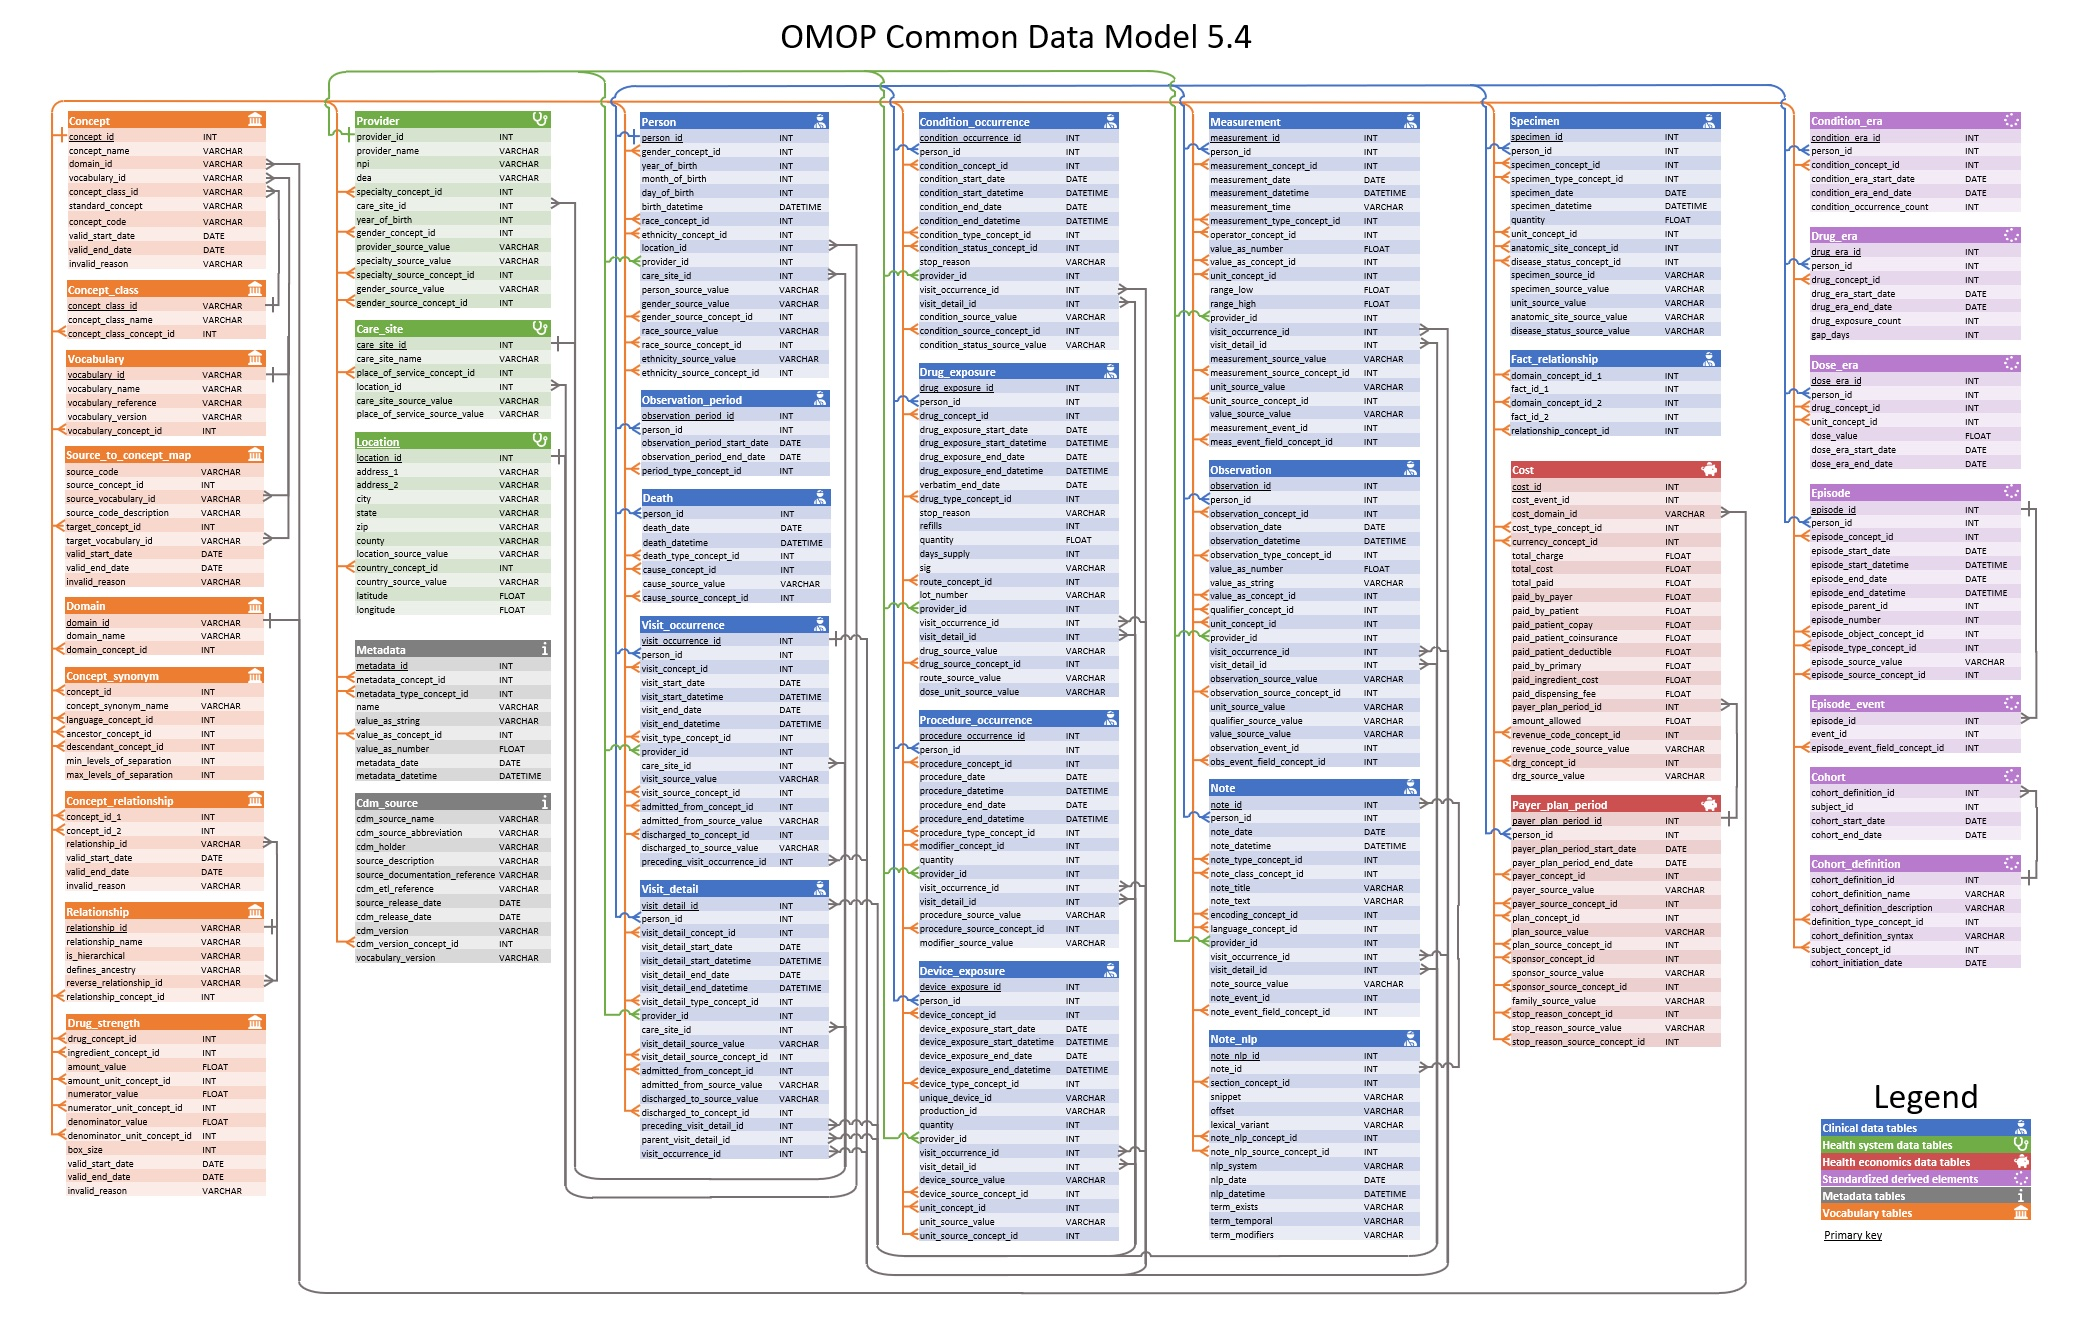
\includegraphics[width=1\textwidth]{figures/cdm_ER.jpg}
     \caption{Modelo Entidad-Relación del CDM v5.4. Extraída de la página de github del CDM \parencite{gitPagesCMD}}
    \label{fig:cdm_ER}
\end{figure}

El modelo se comprende de 39 tablas agrupadas en seis grupos, de los cuales se destaca la importancia de tres: Datos clínicos estandarizados (\textit{Standardized clinical data}, en azul), Vocabularios estandarizado (\textit{Standardized vocabularies}, en naranja) y Elementos derivados estandarizados (\textit{Standardized derived elements}, en morado). El grupo más importante es el de datos clínicos, que contiene la tabla Persona (\textit{Person}), por la característica centrada en el paciente del modelo.

Cada evento clínico se registra en el modelo como un \textbf{Concepto} (\textit{Concept}), perteneciente al grupo del Vocabulario estandarizado (en naranja). Además, cada concepto está ligado a un \textbf{Dominio} que especifica a qué tipo de información clínica corresponde dicho concepto. A continuación se muestra una tabla con los 30 dominios existentes y la cantidad de conceptos que tiene asociado cada uno.

\begin{figure}[H]
    \centering
    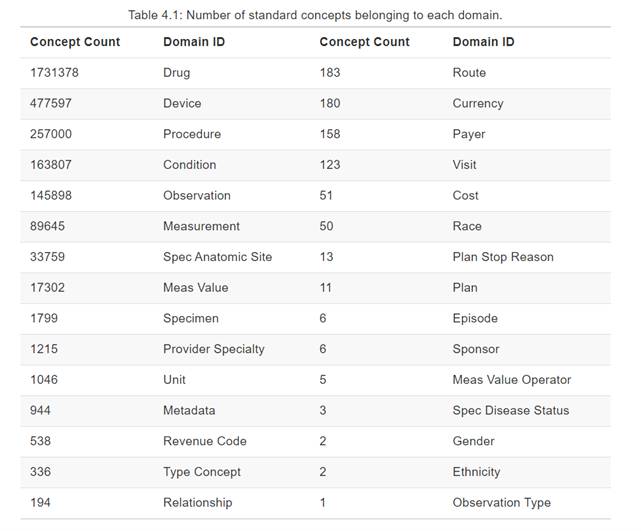
\includegraphics[width=0.80\textwidth]{figures/cdm_domains.png}
     \captionof{table}{Dominios del CDM v5.4. Extraída del Libro de OHDSI \parencite{OHDSIbook}}
    \label{fig:cdm_domains}
\end{figure}

La información que contiene cada dominio se puede inferir fácilmente de la traducción al español del nombre por lo que no se va a hacer hincapié en ello. No obstante, se puede encontrar más información en \parencite{OHDSIbook}, \parencite{gitPagesCMD} o \parencite{CDMinteractive}.

\subsection{Vocabulario}\label{subsec:07vocab}

El Vocabulario es otro de los elementos centrales del Modelo de Datos Común de OMOP y una gran herramienta de estandarización e interoperabilidad entre sistemas. Como se ha comentado en varias ocasiones, actualmente hay muchos estándares distintos en funcionamiento que establecen las terminologías de los eventos clínicos (por ejemplo LOINC, SNOMED CT, RxNorm...). El beneficio del Vocabulario de OMOP es que integra todos los vocabularios ya existentes en un único \textbf{Vocabulario estándar}, a través de la referenciación entre \textbf{conceptos estándar} (pertenecientes a OMOP) y conceptos no estándar (pertenecientes a vocabularios alternativos).

El Vocabulario de OHDSI, por tanto, impera sobre un conjunto de vocabularios, respetando las diversas procedencias de cada término pero mapeándolos a un único vocabulario estándar. \textbf{Cada concepto no estándar está asociado a un concepto estándar} y esta es la clave del Vocabulario. 

Como todas las herramientas de la comunidad, la información acerca de este está disponible online de forma pública en el capítulo 5 del Libro de OHDSI \parencite{OHDSIbook} y en la página de github del CDM \parencite{gitPagesCMD}. Por otra parte, existe un buscador online de términos en el Vocabulario de OMOP denominado ATHENA \parencite{ATHENAweb}. 

\begin{figure}[H]
\centering
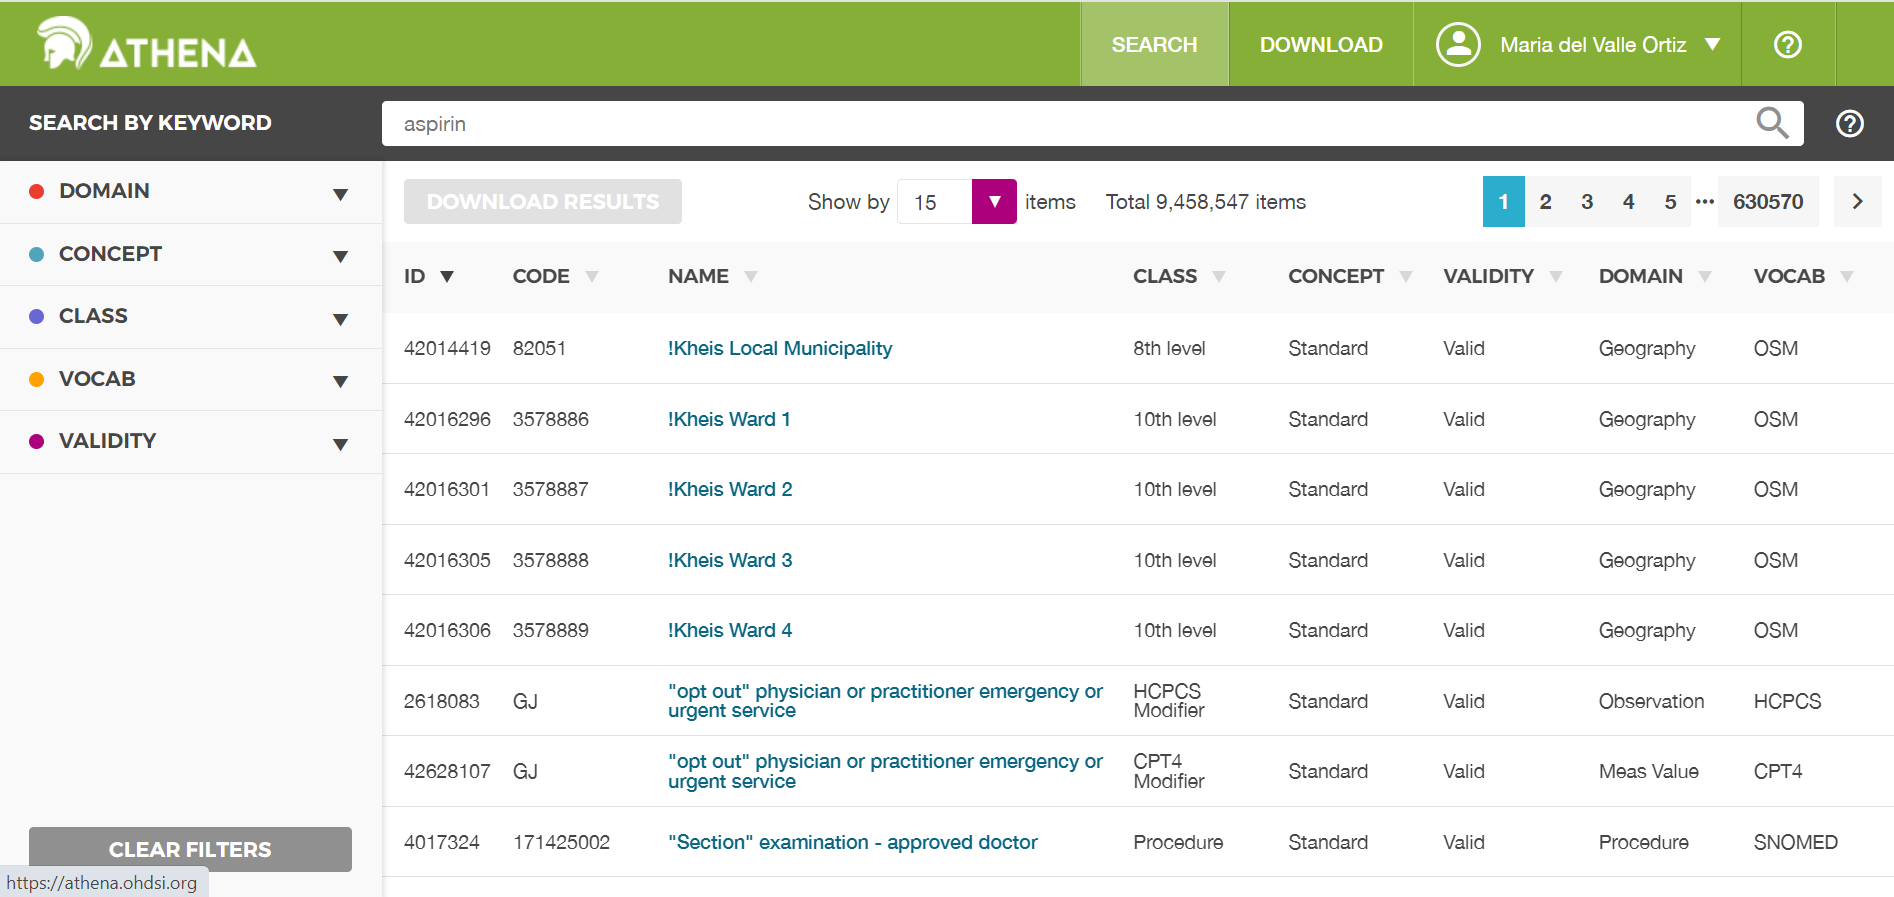
\includegraphics[width=1\textwidth]{figures/ATHENAcap.png}
     \caption{Captura de pantalla del menú principal de ATHENA}
    \label{fig:ATHENAcap}
\end{figure}

Actualmente hay más de nueve millones de términos registrados en el Vocabulario de OMOP, como se muestra en la Figura \ref{fig:ATHENAcap} ''Captura de pantalla del menú principal de ATHENA'', y 155 vocabularios distintos coexisten juntos en el estándar, de los cuales al menos 30 son vocabularios internos de OMOP.

%\textcolor{red}{- lA RELACIÓN QUE GUARDAN LOS CONCEPTOS ENTRE SÍ ES JERARQUICA}

\section{Herramientas de OHDSI} \label{sec:07herramientas}

OHDSI proporciona un conjunto de herramientas para facilitar la realización de los estudios e investigaciones a raíz de los datos clínicos y fomentar la interoperabilidad entre estos, aportando un estándar de herramientas. 

Las herramientas que proporciona la organización están disponibles públicamente online y de forma gratuita y son desarrolladas por los propios miembros de la comunidad. Entre todas las herramientas, para la realización de este proyecto se destaca la herramienta de análisis de datos clínicos ATLAS, aunque también existen otras herramientas importantes de forma indirecta que se describen a continuación.

\subsection{ATLAS} \label{subsec:07ATLAS}

ATLAS es la herramienta de OHDSI por excelencia porque es la que estandariza el análisis observacional una vez que la base de datos está convertida al modelo OMOP. La documentación oficial sobre ATLAS se encuentra en el capítulo 8 del Libro de OHDSI y en su repositorio de github \parencite{githubATLAS}. Además, aparte de la documentación oficial, hay montones de información esparcidas por la red sobre ATLAS, en publicaciones científicas, foros de OHDSI, videotutoriales en youtube y un largo etcétera.

\begin{figure}[H]
\centering

\includegraphics[width=0.25\textwidth]{figures/ATLASlogo.png}
     \caption{Logo de ATLAS. Extraída del repositorio de github \parencite{githubATLAS}}
    \label{fig:ATLASlogo}
\end{figure}

Un importante promotor del uso de ATLAS es la red europea de datos EHDEN (véase \ref{sec:01EstadoArte} ''Estado del arte''). En esta línea, también la plataforma EHDEN Academy también ofrece cursos gratuitos sobre el uso de ATLAS y otras herramientas OHDSI.

\subsubsection{Características y beneficios de su uso}

El uso de ATLAS es beneficioso para la comunidad científica debido principalmente a su naturaleza \textit{open-source}, \textit{low-code} y la reproducibilidad que ofrece para los estudios:

\begin{enumerate}[label=\roman*.]

    \item \textbf{Open source}. ATLAS se presenta como una herramienta disponible públicamente online, configurable gracias a su característica de cógido abierto, que expone toda su información y el propio código que la compone en los repositorios de github de la organización y, por si fuera poco, cuenta con el apoyo de un equipo de desarrolladores pendiente en los foros e \textit{issues} que se reportan vía github para solucionar las dudas que tengan los implementadores. 

    \item \textbf{Low-code}. Por otro lado, no requiere de conocimientos expertos de programación, puesto que es \textit{low-code}. La herramienta se implementa sobre la Biblioteca de Métodos de OHDSI, con soporte para análisis en R, pero no requiere programación directa sino que ofrece una interfaz gráfica e intuitiva para el analista de datos. Además, el código que subyace al análisis es fácilmente exportable, siempre estructurado según el mismo estándar, favoreciendo la interoperabilidad del mismo.

\begin{figure}[H]
\centering
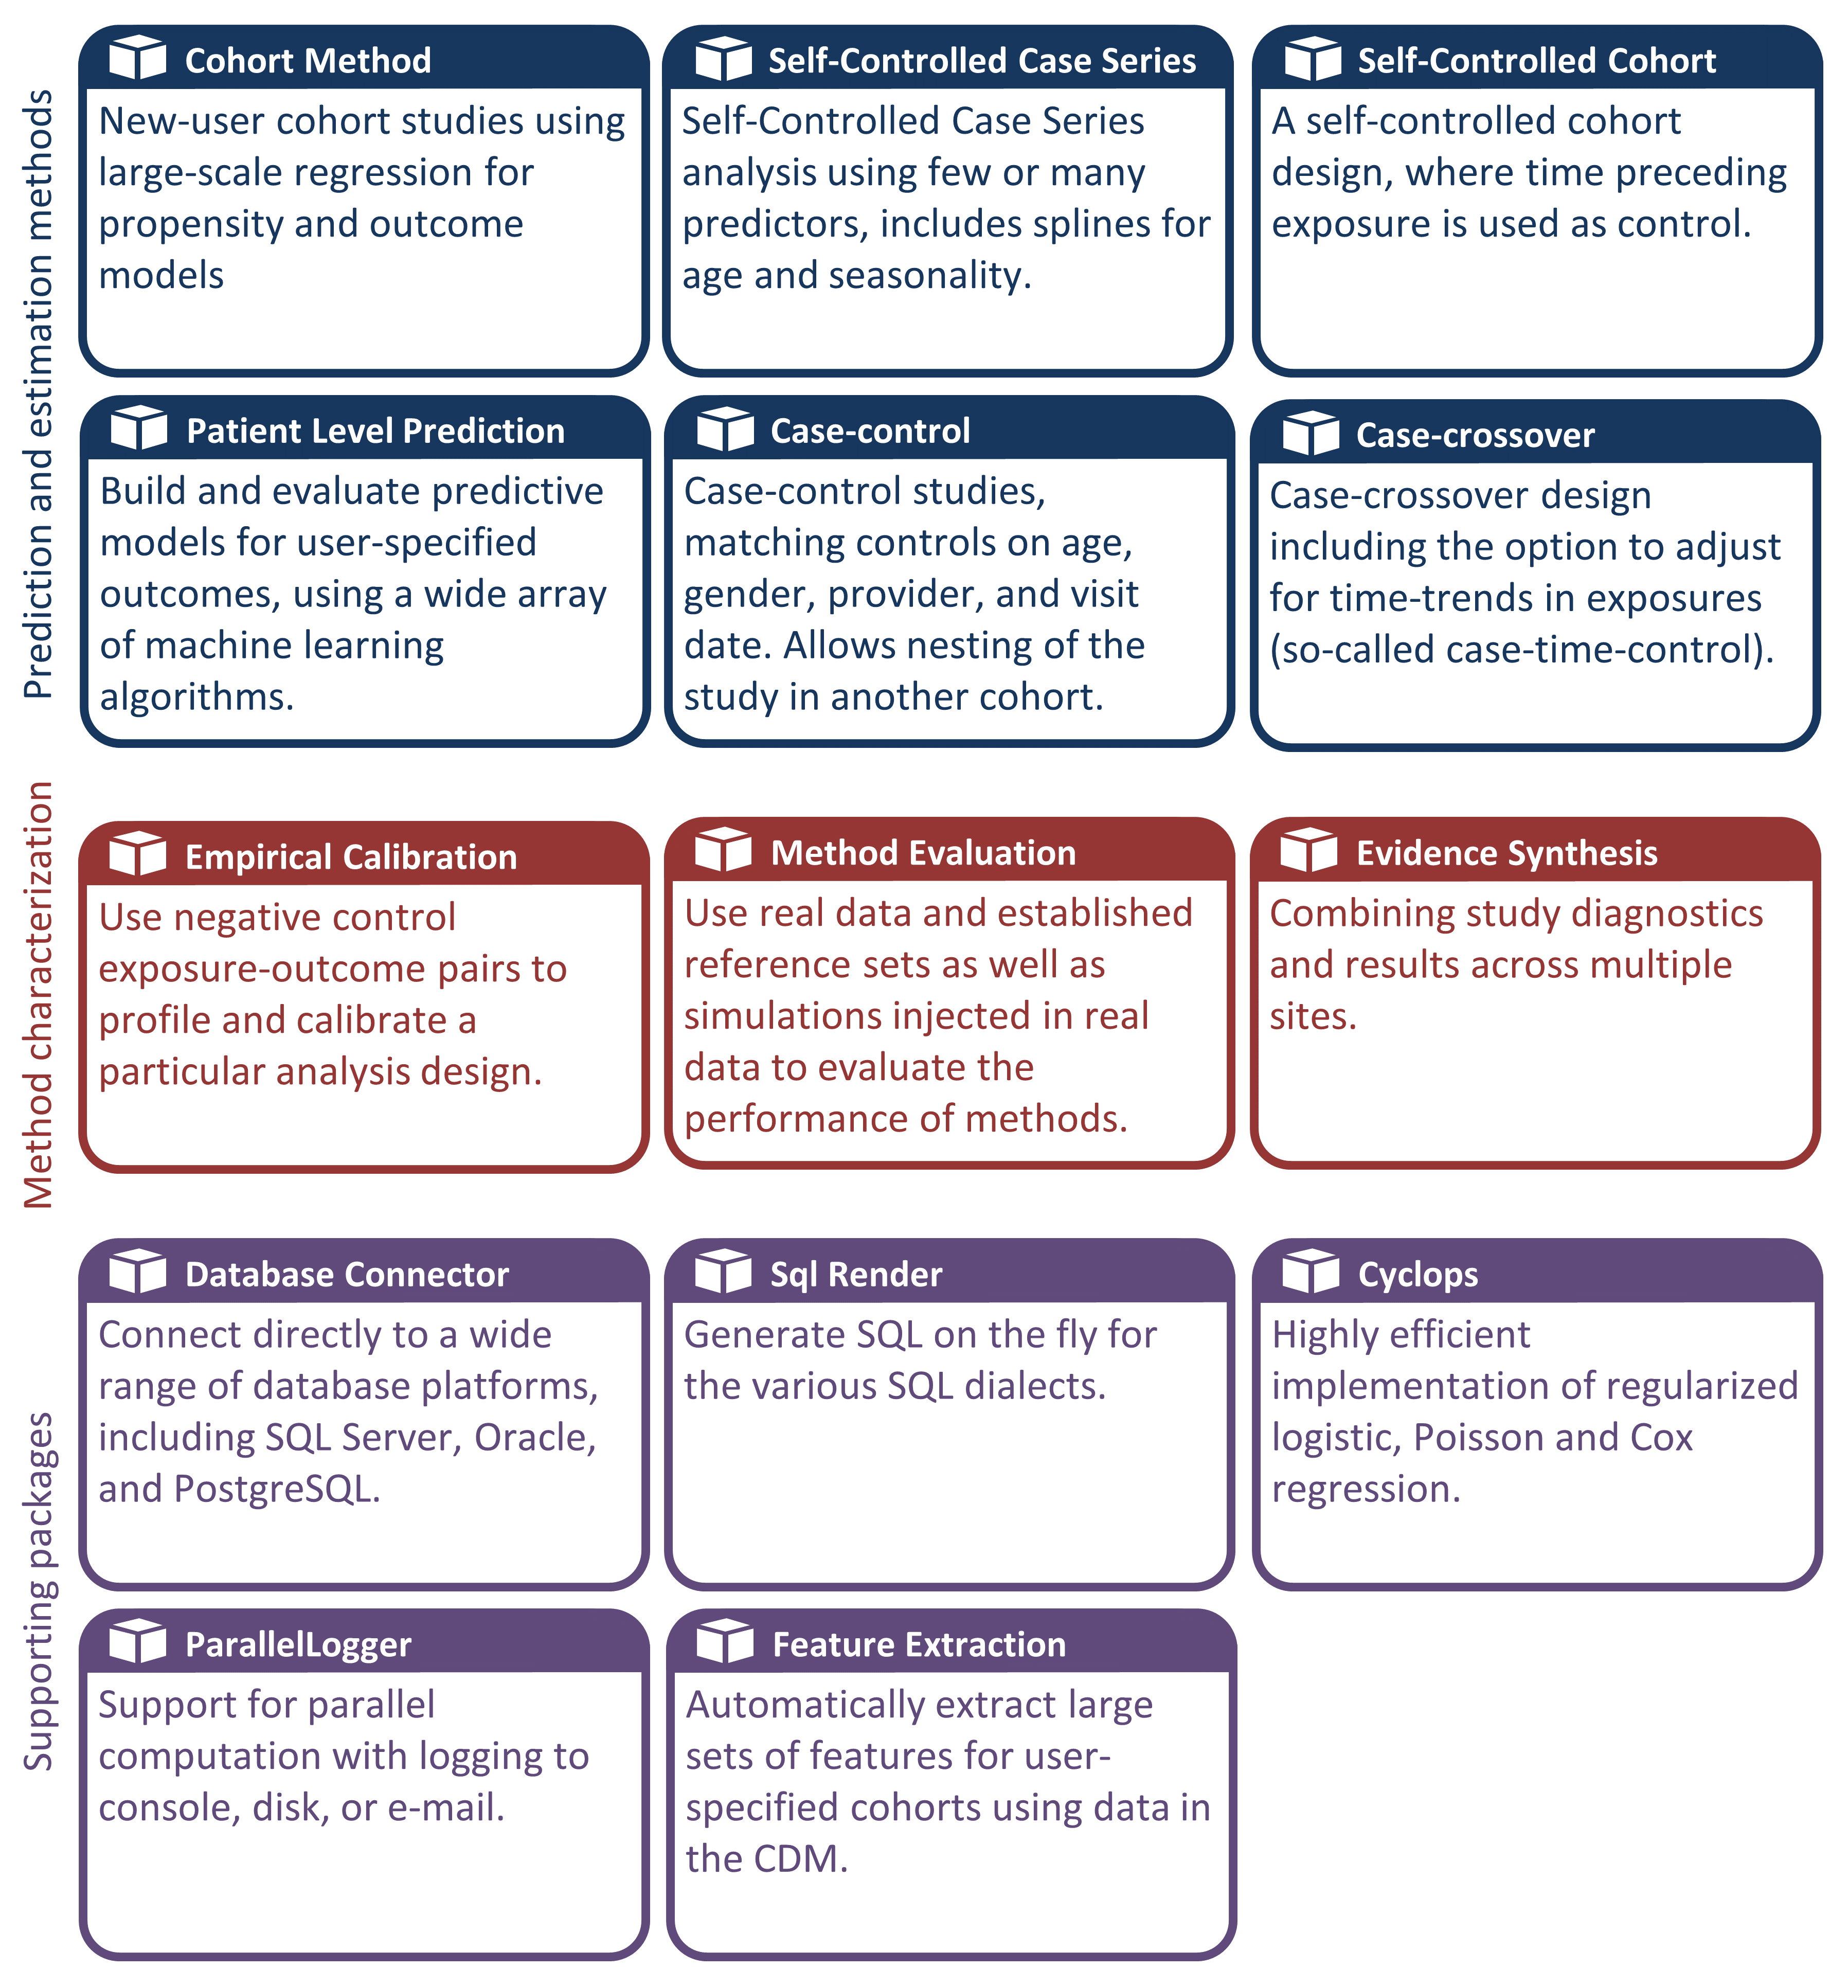
\includegraphics[width=0.70\textwidth]{figures/methodsLibrary.png}
\caption{Biblioteca de Métodos OHDSI. Extraída del Libro de OHDSI \parencite{OHDSIbook}}
\label{fig:methodsLibrary}
\end{figure}
    
     Todo ello no solo facilita la tarea del analista de datos sino que además favorece la interoperabilidad entre los estudios, puesto que todos los estudios que utilizan ATLAS implementan (en una capa inferior) los mismos métodos, el mismo lenguaje de programación y la misma estructura de análisis (véase \ref{sec:05Evidencia} ''¿Cómo generar evidencia?''). 

     \item \textbf{Reciclabilidad}. Por último, otro beneficio es que gracias a estas características ATLAS permite diseñar estructuras para el estudio de los datos que puedan utilizarse en diferentes bases de datos distintas. Volviendo al ejemplo de la plancha en \ref{sec:05OHDSI} ''¿Qué es OHDSI?'', esto quiere decir que una misma plancha (o estudio) puede conectarse a cualquier enchufe de cualquier región (a cualquier base de datos). ATLAS está intrínsicamente configurada para diseñar análisis reproducibles, por lo que los elementos que se configuran durante un análisis de datos (grupos de cohortes, estimadores, predictores, grupos de conceptos...) se pueden exportar fácilmente a modo de estructura general e implementarse sobre otro estudio que, aunque posea datos distintos ejecute ATLAS. Por tanto las estructuras más eficientes que se utilizen en un análisis remoto, pueden compartirse en la red de la comunidad y ser utilizados en cualquier nodo y cualquier estudio, favoreciendo la reciclabilidad, reproducibilidad e interoperabilidad del estudio.
    
\end{enumerate}

\subsubsection{Aspectos técnicos}

En cuanto a los aspectos técnicos, ATLAS se despliega como una herramienta basada en web, normalmente alojada en un servidor Apache, combinada con la WebAPI de OHDSI. Generalmente se recomienda su despliegue en Google Chrome. Además la herramienta puede implementarse de forma pública a través de internet o tras el firewall de la red privada de una organización, según las necesidades de la entidad que lo implementa.

Sin embargo, es importante recalcar que tanto ATLAS como la mayoría de las herramientas de OHDSI no consiste en un archivo ejecutable aislado sino en una aplicación contenida y dependiente de un ecosistema completo basado en web. La dependencia principal y red que sostiene a ATLAS es la \textbf{WebAPI}.

\begin{figure}[H]
    \centering
    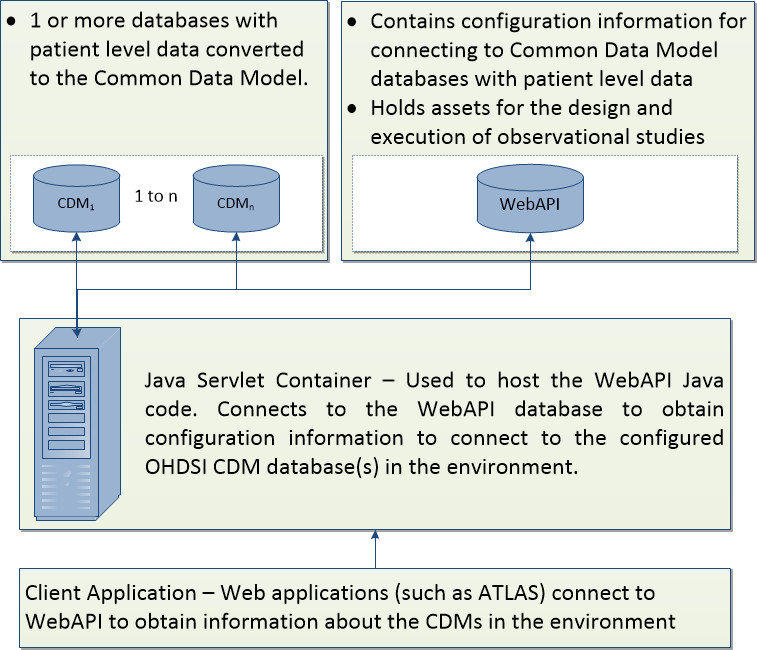
\includegraphics[width=0.700\textwidth]{figures/webAPIwiki.png}
     \caption{Estructura de la WebAPI. Extraída de la wiki de github \parencite{githubWebAPIwiki}}.
    \label{fig:webAPIwiki}
\end{figure}

Tal y como se muestra en la Figura \ref{fig:webAPIwiki} ''Estructura de la WebAPI'', la WebAPI es la aplicación que proporciona los servicios RESTful para que la herramienta pueda interactuar con las bases de datos \parencite{githubWebAPIwiki}. Por tanto su relación con ATLAS es estrictamente necesaria. ATLAS no es una herramienta aislada sino un eslabón del ecosistema OHDSI.

Por otra parte, la herramienta en sí se muestra a través de una interfaz gráfica, que proporciona un estrecho menú lateral con 15 herramientas para el análisis de datos. La interfaz de la herramienta seleccionada se muestra en el lado derecho, como se muestra en la Figura \ref{fig:ATLASdemoHome} ''Captura de pantalla del menú principal de ATLAS demo''.

\begin{figure}[H]
\centering
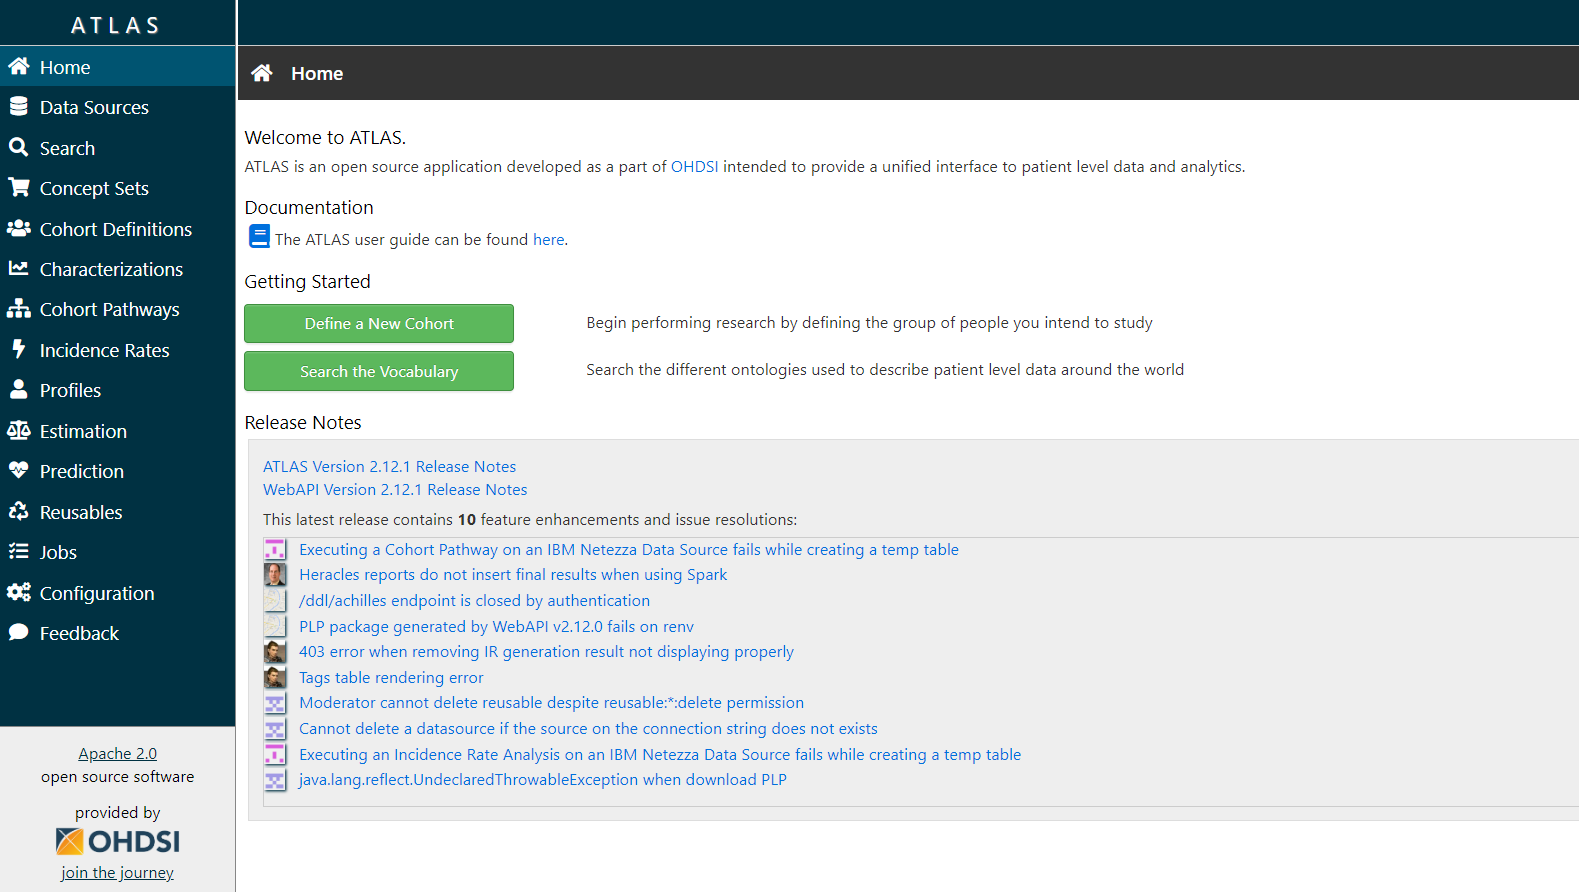
\includegraphics[width=0.90\textwidth]{figures/ATLASdemoHome.png}
     \caption{Captura de pantalla del menú principal de ATLAS demo}
    \label{fig:ATLASdemoHome}
\end{figure}

Recientemente, en diciembre de 2023, ATLAS lanzó su versión 2.14.1 que está en correcto funcionamiento y es la que se utiliza en el desarrollo del Trabajo Fin de Grado. Más información sobre los aspectos técnicos de la herramienta se encuentran en el repositorio de github \parencite{githubATLAS}.

\subsubsection{Estrategias de Implementación}

La implementación de ATLAS en una organización puede ser una tarea complicada por su dependencia con la WebAPI, la Biblioteca de Métodos y otras dependencias al ecosistema OHDSI. 

No obstante, la organización ha desarrollado varias iniciativas que facilitan su implementación y accesibilidad, para no crear obstáculos en la promoción del uso de la herramienta. Estas iniciativas se describen a continuación.

\begin{enumerate}[label=\alph*.]

    \item \textbf{ATLAS demo} \parencite{ATLASdemo}. En primer lugar, esta es una herramienta muy fácilmente accesible que proporciona la comunidad científica para tomar un primer contacto con la herramienta. En este caso, la herramienta es accesible a través del navegador web, publicamente a través de Internet. Cualquier usuario de internet tiene acceso a la herramienta demo. Se le denomina demo porque se sobreentiende que su uso es principalmente educativo o formativo, aunque verdaderamente ofrece todas las capacidades de la herramienta y los análisis que con ella se realizan, podrían reutilizarse en estudios más complejos o de organizaciones privadas.

    \item \textbf{ATLAS Docker}. Por otro lado, también muy fácilmente implementable se presenta \textbf{Broadsea} \parencite{githubBroadsea}, que consiste en la virtualización del ecosistema OHDSI en un multicontenedor Docker. Gracias a la facilidad del uso de las tecnologías Docker, esta forma de implementar el ecosistema es bastante sencilla, permitiendo además añadir nuevas configuraciones más complejas (si fuese necesario) añadiendo o eliminando contenedores. Para realizar la parte práctica de este trabajo se emplea la tecnología Docker de Broadsea para implementar ATLAS. A la herramienta ATLAS desplegada con Broadsea, frecuentemente se le denominará a lo largo del documento \textit{ATLAS Broadsea}. El TFG presenta un documento anexo bastante complejo enteramente dedicado a la instalación, despliegue y configuración del entorno Broadsea (véase anexo \ref{anexo:manual} ''Manual de instalación, despliegue y configuración de ATLAS Broadsea''). Adicionalmente, la arquitectura de Broadsea también se presenta en \ref{sec:08Broadsea} ''Arquitectura de Broadsea''.

    \item \textbf{ATLAS Amazon Web Services}. Otra alternativa que propone la organziación, en colaboración con Amazon, es la virtualización del ecosistema en el entorno de computación en la nube de Amazon Web Services (AWS). Para ello se ofrecen los entornos \textit{OHDSI-in-a-Box} \parencite{githubOHDSIBox} y \textit{OHDSIonAWS} \parencite{githubOHDSIAWS}. OHDSI-in-a-Box se crea específicamente como un entorno de aprendizaje y se utiliza en la mayoría de los tutoriales proporcionados por la comunidad OHDSI mientras que OHDSIonAWS es una arquitectura de referencia para entornos OHDSI de clase empresarial, multiusuario, escalables. Por las restricciones intrínsecas al uso de AWS, estas alternativas han sido rechazadas para ser empleadas en el TFG.
    
    \item \textbf{ATLAS Azure}. Por último, \textit{OHDSI on AZURE} \parencite{OHDSIonAzure} es otra alternativa de virtualización pero a través de la plataforma Microsoft de Azure. No obstante, esta alternativa es la menos común.
    
\end{enumerate}

\subsubsection{Herramientas embebidas}

Si bien las herramientas del ecosistema de OHDSI no son totalmente aisladas, ATLAS presenta en su propia interfaz acceso a dos de estas herramientas de forma íntegra, para facilitar la eficiencia y rapidez en el análisis. Estas herramientas son las siguientes:

\begin{itemize}

    \item \textbf{ACHILLES} \parencite{githubACHILLES}. Esta herramienta, de las siglas \textit{Automated Characterization of Health Information at Large-Scale Longitudinal Evidence Systems}, en español Caracterización automatizada de la información sanitaria en sistemas de evidencia longitudinal a gran escala, sirve para caracterizar y/o obtener un reporte estadístico de la base de datos estandarizada que se va a utilizar para el estudio. Intrínsicamente es una librería de R que se implementa como una opción del menú lateral \textit{Data Sources} de ATLAS.
    \item \textbf{ATHENA} \parencite{githubATHENA}. Esta herramienta sirve para realizar búsquedas dinámicas en el Vocabulario de OMOP (véase \ref{subsec:07vocab} ''El Vocabulario''). Está implementada en ATLAS en la opción \textit{Search} del menú lateral. Además, se puede acceder a ella online de forma externa a través de su propia página web \parencite{ATHENAweb}.
    
\end{itemize}


\subsection{Otras herramientas} \label{subsec:07otrasHerramientas}

El ecosistema de OHDSI presenta gran cantidad de herramientas adicionales. A continuación se presentan otras herramientas que aunque no se utilizan directamente, son importantes para realizar un análisis de datos completo. 

\begin{itemize}
    
    \item \textbf{HADES} \parencite{githubHADES}. HADES, del inglés\textit{ Health Analytics Data-To-Evidence Suite} y en español Suite de análisis sanitario de datos a evidencia, es el nombre con el que se denomina a la herramienta que implementa el paquete R con la Biblioteca de Métodos de OHDSI (ver Figura \ref{fig:methodsLibrary} ''Biblioteca de Métodos OHDSI''). Se puede instalar como un entorno independiente mediante Java y Rtools para implementar análisis mediante código estandarizado (véase Figura \ref{fig:analysisImplementations} ''Tres vías para la implementación de un análisis observacional''). No se utiliza en el TFG más alla de la implementación subyacente de las bibliotecas en ATLAS.
    \item \textbf{Rabbit tools y Usagi} \parencite{OHDSIsoftTools}. Estas herramientas en conjunto llevan a cabo el proceso de ETL, para omopizar las bases de datos al Modelo de Datos Común de OMOP. Las herramientas son tres: White-Rabbit, Rabbit-In-Hat y Usagi. No se utiliza directamente en el TFG porque el dataset utilizado para el análisis ya estaba previamente omopizado.
    \item \textbf{Data Quality Dashboard} \parencite{githubDQD}. Esta herramienta, en español Panel de control de calidad de los datos, pertenece a un paquete de HADES aunque implementado como una interfaz gráfica aparte para facilitar su acceso online. Tal y como su nombre indica sirve para automatizar la tarea de comprobación de la calidad de los datos, un paso previo fundamental antes de realizar un análisis de datos. Tampoco se utiliza directamente para el TFG porque este estudio se llevó a cabo durante la omopización del dataset.
        
\end{itemize}

\section{Programas informáticos empleados} \label{sec:07programas}

Los programas informáticos que han permitido el despliegue de este entorno tecnológico que envuelve al sistema son los siguientes:  Google Chrome, Docker, PostgreSQL y Github.


\subsubsection{Google Chrome}

Google Chrome es el navegador web de Google que permite el acceso a internet y la búsqueda en la web a través de una interfaz amigable e intuitiva \parencite{GoogleChrome}. 

Chrome es el navegador recomendado por OHDSI para desplegar las herramientas de su ecosistema y más especialmente en el despliegue de Broadsea, permitiendo el acceso al servidor donde se aloja el sistema. Por tanto su uso ha sido muy relevante como portal de acceso a las herramientas OHDSI.


\subsubsection{Docker}

Docker es una plataforma abierta para desarrollar, enviar y ejecutar aplicaciones. Docker le permite separar sus aplicaciones de su infraestructura para que pueda entregar software rápidamente. Con Docker, puede administrar su infraestructura de la misma manera que administra sus aplicaciones \parencite{DockerWebsite}.

De esta forma, Docker permite empaquetar y ejecutar aplicaciones en contenedores, entornos poco aislados pero seguros. Esto posibilita la ejecución de múltiples contenedores simultáneamente en un mismo host, sin depender de lo instalado en él. Los contenedores son ligeros y contienen todo lo necesario para la aplicación, facilitando su compartición y asegurando consistencia entre usuarios. 

El uso de Docker en el desarrollo del proyecto es evidente, es la herramienta que despliega Broadsea y, por consiguiente, ATLAS. El proceso concreto de instalación, despliegue y configuración de Docker así como la explicación detallada de su estructura y archivos más importantes se presenta en el anexo \ref{anexo:manual} ''Manual de instalación, despliegue y configuración de ATLAS Broadsea''.

\subsubsection{PostgreSQL}

PostgreSQL es un potente sistema de base de datos relacional de objetos de código abierto que utiliza y amplía el lenguaje SQL combinado con muchas funciones que almacenan y escalan de forma segura las cargas de trabajo de datos más complicadas \parencite{PostgreWebsite}.

El uso de postgre es fundamental para la implementación correcta de Broadsea, puesto que su base de datos se implementa según PostgreSQL. Las bases de datos externas que se interactúan con la WebAPI pueden estar en otros lenguajes relacionales, pero el sistema de Broadsea intrínsicamente solo se sostiene sobre Postgre.

El proceso concreto de instalación, despliegue y configuración de la base de datos Postgre se realiza a través de la interfaz visual de pgAdmin 4.0 \parencite{pgAdminWebsite} y la explicación detallada de su estructura y archivos más importantes se presenta en el anexo \ref{anexo:manual} ''Manual de instalación, despliegue y configuración de ATLAS Broadsea''.

\subsubsection{Github}

GitHub es una plataforma para desarrolladores que les permite crear, almacenar, gestionar y compartir su código. Utiliza el software Git, proporcionando control de versiones distribuido, además de control de acceso, seguimiento de errores, solicitudes de funciones de software, gestión de tareas, integración continua y wikis para cada proyecto \parencite{GithubWikipedia}.

El uso de Github es muy recomendado debido a que la mayor parte de la información sobre OHDSI y sus herramientas se encuentran en internet disponibles en repositorios de Github (véase \ref{sec:05OHDSI} ''¿Qué es OHDSI?''). 

Además, siguiendo esta iniciativa de OHSI, para desarrollar este Trabajo Fin de Grado se ha creado un repositorio de Github específico \parencite{vallealonsodc} que contiene toda la documentación relevante a su desarrollo (archivos latex, pdf...) y archivos de variables de entorno o scripts utilizados durante la configuración del entorno del sistema o la realización del análisis de datos.   


\section{Conclusiones} \label{sec:07conclusiones}

En esta sección se concluye que el entorno de trabajo del proyecto está enmarcado en el entorno de estándares y herramientas de la organización OHDSI, desplegados a través de una serie de programas informáticos. 

Conocer el entorno de trabajo del proyecto y de OHDSI es gran relevancia puesto que no puede entenderse ATLAS sin conocer estos otros. 

    \chapter{Arquitectura del Sistema}\label{cap:08arquitectura}

Este capítulo se divide en cuatro secciones: \ref{sec:08intro} Introducción, \ref{sec:08teorica} Arquitectura teórica del sistema y \ref{sec:08Broadsea} Arquitectura de Broadsea y \ref{sec:08conclusiones} Conclusiones.

\section{Introducción} \label{sec:08intro}

La implementación del ecosistema de herramientas OHDSI y ATLAS puede ser una ardúa tarea. En el contexto de desarrollo del Trabajo Fin de Grado junto a las prácticas en empresa en el Hospital Virgen del Rocío, la dificultad de la tarea se ve exponencialmente aumentada debido a los grandes protocolos de seguridad y privacidad de la administración pública. Por ello, se ha seleccionado el despliegue de las herramientas OHDSI a través del sistema Docker de Broadsea, que presenta una vía sencilla para realizar esta labor. 

Broadsea es un proyecto basado en Docker que permite desplegar todo el entorno de herramientas, configuraciones y dependencias OHDSI de la manera más sencilla hasta el momento. Por tanto, \textbf{el sistema se trata de una virtualización en Docker del entorno de herramientas OHDSI}.

\begin{figure}[H]
    \centering
    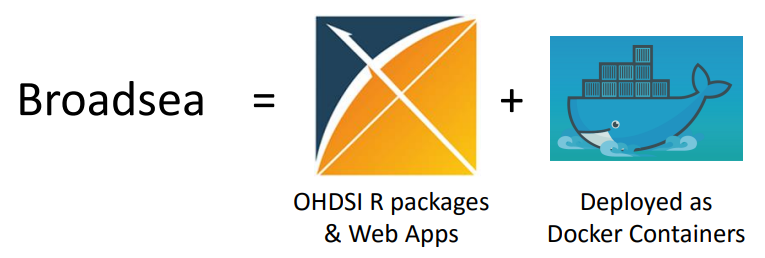
\includegraphics[width=0.70\textwidth]{figures/broadseaEq.png}
    \caption{Esquema sencillo de Broadsea. Extraída de \parencite{Broadsea3PPTX}.}
    \label{fig:broadseaEq}
\end{figure}

En la sección \ref{sec:08teorica} ''Arquitectura teórica del sistema'' se presentan los aspectos teóricos fundamentales sobre virtualización y componentes de los sistemas docker y en la sección \ref{sec:08Broadsea} ''Arquitectura tecnológica de Broadsea'' se presenta la arquitectura específica de Broadsea.

No obstante, la arquitectura del sistema también se presenta en mayor profundidad técnica en el Anexo \ref{anexo:manual} ''Manual de instalación, despliegue y configuración de ATLAS Broadsea''.

\section{Arquitectura teórica del sistema} \label{sec:08teorica}

El sistema se implementa mediante virtualización en Docker y una arquitectura en tres niveles o \textit{three-tier}, donde se diferencian al cliente, frontend y backend. Esta arquitectura se describirá de forma general utilizando el esquema de la Figura \ref{fig:threeTierValle}.

\begin{figure}[H]
    \centering
    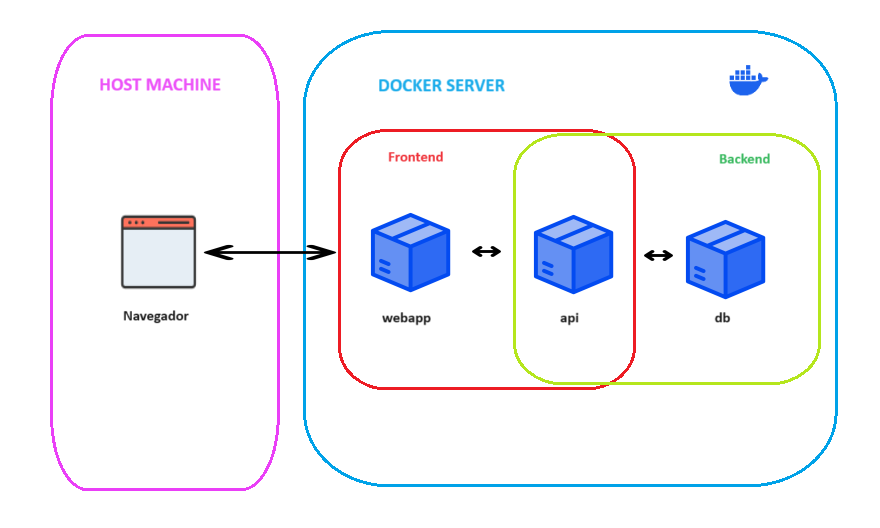
\includegraphics[width=0.90\textwidth]{figures/threeTierValle.png}
    \caption{Esquema de arquitectura \textit{three-tier} en Docker.}
    \label{fig:threeTierValle}
\end{figure}

En primer lugar, la virtualización obliga a diferenciar entre una maquina local o anfitriona (\textit{host machine}, en rosa) y una maquina virtual que provee el servicio docker (\textit{docker service}, en azul). 

\begin{enumerate}

    \item \textbf{La máquina local.} La máquina local es la propia máquina del usuario. Se le denomina anfitriona porque aloja en su interior a la máquina virtual. La máquina local cede un servidor y un puerto a la máquina virtual para que el usuario final pueda acceder al sistema a través de la dirección del servidor en que se aloja, típicamente accediendo mediante un navegador web. El acceso mediante el navegador web es lo que se denomina la capa cliente, pues es la interfaz que permite al usuario acceder al sistema. 

    \item \textbf{La máquina virtual.} La máquina virtual es el sistema virtualizado en Docker. Es el sistema que contiene toda la lógica de la aplicación y los datos empaquetado en un multicontenedor Docker, en este caso el multicontenedor es el propio sistema Broadsea. Está compuesto por tres nodos la \textit{webapp}, la \textit{api} y la \textit{db} que conforman las dos capas restantes de la arquitectura: el frontend y el backend.
    
\end{enumerate}

Por tanto, a nivel de aquitectura del sistema en sí, se encuentra la capa cliente (en el \textit{host machine}, en rosa), el frontend (\textit{network-frontend}, en rojo) y el backend (\textit{network-backend}, en verde).

\begin{enumerate}

    \item \textbf{El cliente.} El cliente está alojado en la máquina anfitriona y proporciona el acceso a los servicios virtualizados del sistema a través de la conexión internet con el servidor docker.

     En el caso de Broadsea el navegador deberá ser Google Chrome y la dirección por defecto será http://127.0.0.1:5432.

    \item \textbf{El frontend.} El frontend está alojado en la máquina virtual, es el servicio que guarda la lógica de la aplicación que se muestra al usuario. Se compone de la \textit{webapp}, que contiene la aplicación como tal, y la \textit{api}. que es la red que permite establecer interconexiones entre la aplicación lógica y la base de datos; entre el frontend y el backend.

    En el caso de Broadsea la webapp y la api se combinan en el componente de la WebAPI, que permite el acceso a la aplicación de ATLAS y maneja las conexión con las bases de datos del backend.

    \item \textbf{El backend.} El backend está alojado en la máquina virtual, es el servicio que aloja la base de datos sobre la que se sostiene la aplicación. Se compone de la \textit{api} y la \textit{db}. De igual forma que en el frontend, la api es la red que permite la interconexión entre los componentes del sistema, en este caso con la base de datos, que puede ser una o varias.

    En el caso de Broadsea, las bases de datos deberán estar estandarizadas a OMOP y podrán encontrarse en el propio servidor Docker, como es el caso de Eunomia, o en servidores externos. No obstante, la relación entre cualquier base de datos y ATLAS se realiza a través de la WebAPI.

    
\end{enumerate}

\section{Arquitectura de Broadsea} \label{sec:08Broadsea}

Broadsea es un sistema muy complejo, contenido en un multicontenedor Docker que alberga el ecosistema completo de herramientas OHDSI y sus interconexiones en distintos contenedores. Además, se definen distintos perfiles (\textit{profiles}) para facilitar la instalación de los distintos contenedores. Por ello se le denomina \textit{a-la-carte}. 

Broadsea es el \textit{docker server} al que se refiere la anterior Figura \ref{fig:threeTierValle} ''Esquema de arquitectura three-tier en Docker''. A continuación se muestran todos los contenedores que alberga el sistema de Broadsea.

\begin{figure}[H]
    \centering
    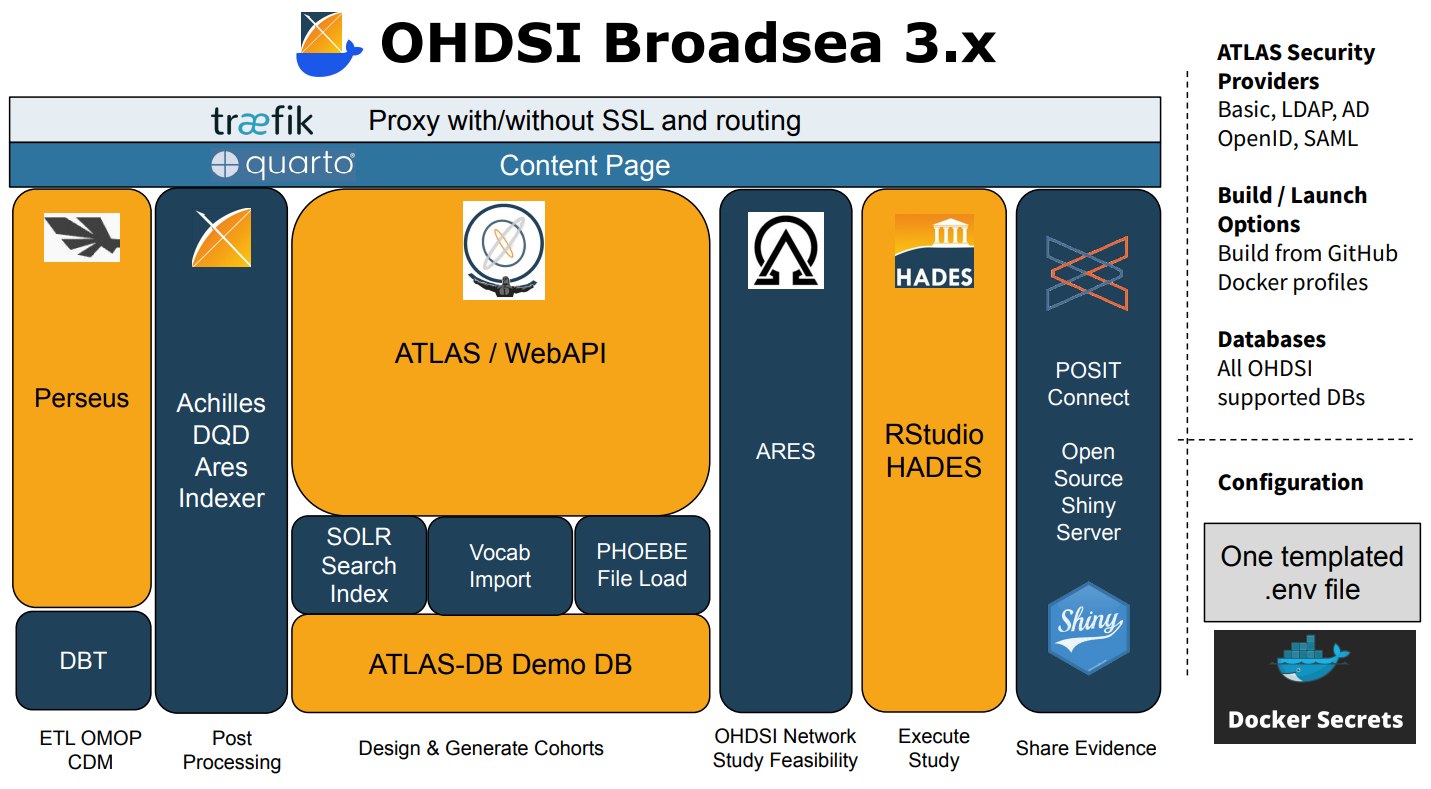
\includegraphics[width=0.90\textwidth]{figures/OHDSIBroadsea3.0.png}
    \caption{Vista general de todos los componentes de Broadsea. Extraída de \parencite{Broadsea3PPTX}.}
    \label{fig:OHDSIBroadsea3.0}
\end{figure}

El despliegue por defecto de Broadsea genera una interfaz de usuario con acceso a tres aplicaciones: ATLAS, HADES y ARES. Para acceder a esta interfaz de usuario basta con buscar en el navegador el servidor y puerto donde se aloja broadsea. Tipicamente el servidor corresponde al \code{localhost} y el puerto \code{5354}, correspondiente a Postgre. La figura a continuación muestra la interfaz principal de herramientas disponibles al acceder a Broadsea desde Chrome.

\begin{figure}[H]
    \centering
    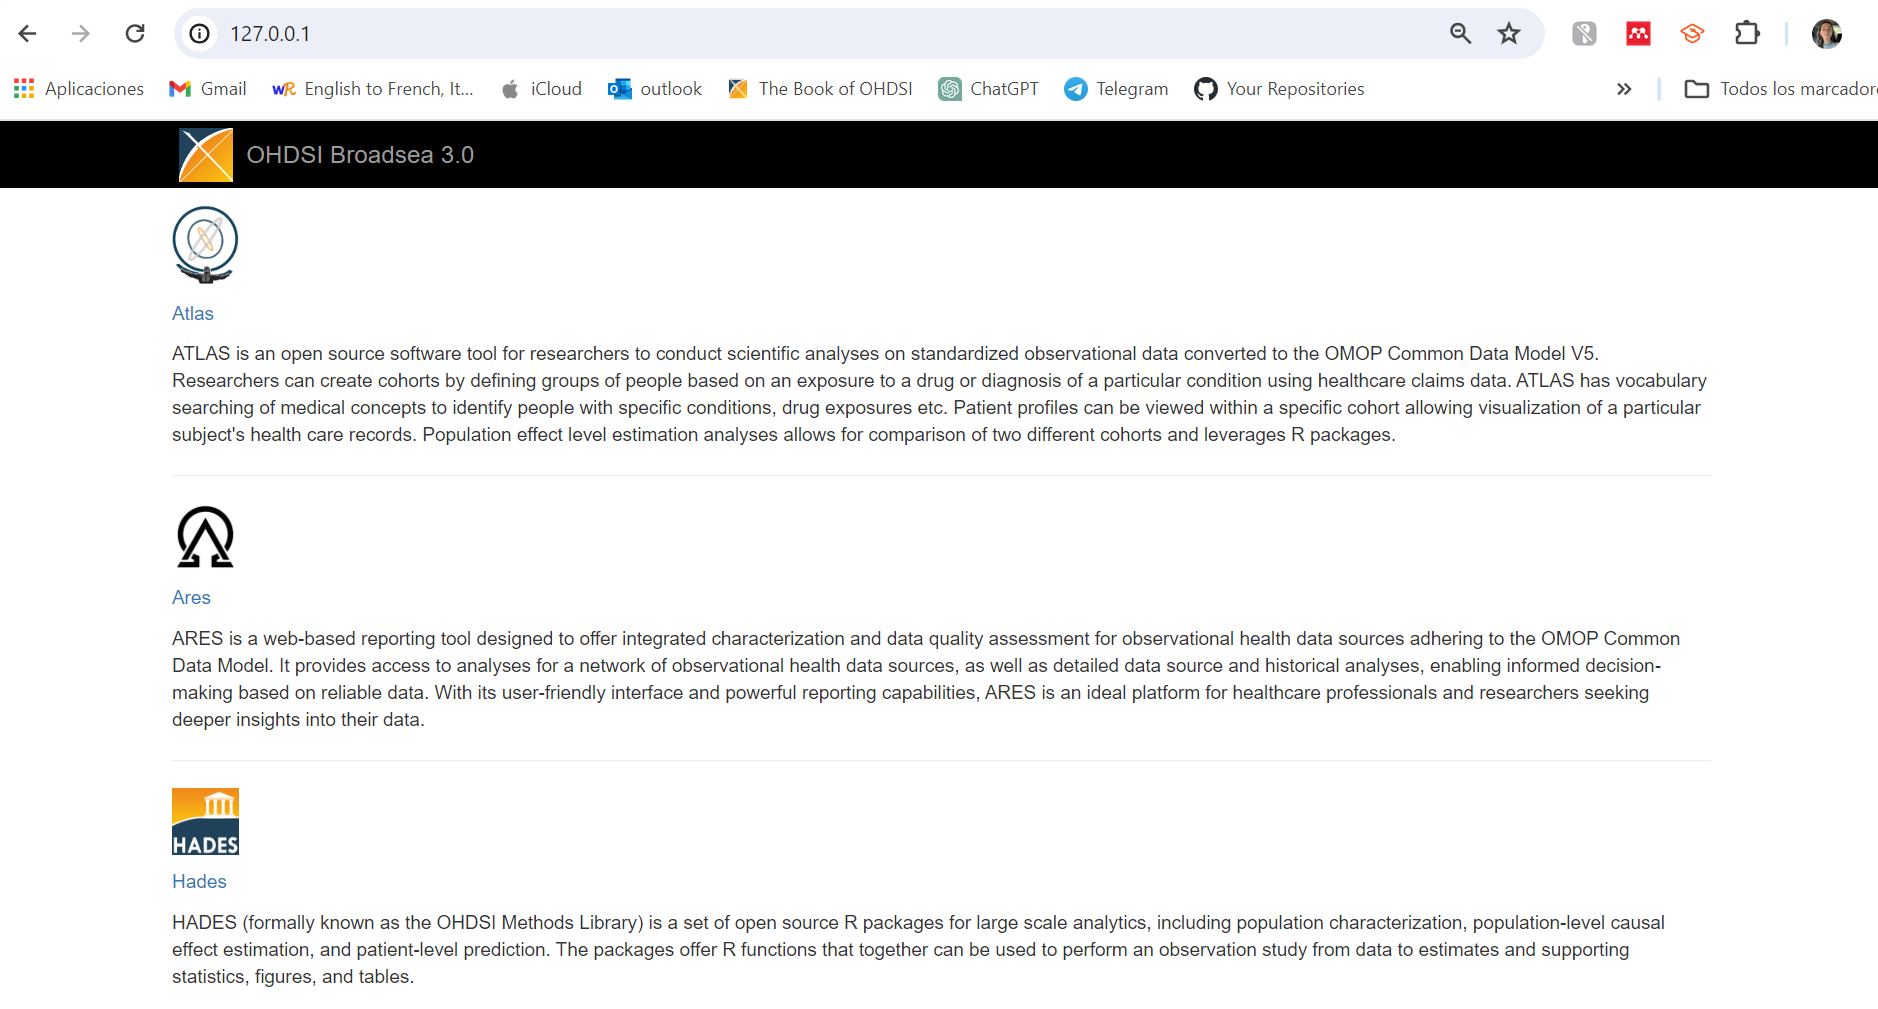
\includegraphics[width=1\textwidth]{figures/homeBroadsea.png}
    \caption{Captura de pantalla del menú principal de Broadsea}
    \label{fig:homeBroadsea}
\end{figure}

Por tanto, haciendo referencia a ambas figuras, se presenta a continuación una breve descripción de cada una de las herramientas accesibles desde el menú principal de Broadsea. En el caso de ATLAS, por su relevancia, se describe la relación de contenedores de Broadsea que participan en su despliegue.

\begin{enumerate}

    \item \textbf{ATLAS}. ATLAS Broadsea despliega todas las funcionalidades de la herramienta de forma local. ATLAS se sostiene sobre la WebAPI y cuenta con la base de datos de Eunomia.
    
    \begin{itemize}
        \item \textbf{WebAPI}. La WebAPI se despliega como un contenedor docker y como un volumen de datos. Además, también se construirá un esquema en la base de datos del servidor Postgre que aloja al contenedor, denominado \code{webapi}. A través de la modificación de este esquema se podrán agregar o eliminar las diferentes fuentes de datos a la herramienta.
        \item \textbf{BD}. Para facilitar el correcto funcionamiento de ATLAS se implementa una base de datos demo que es Eunomia. Esta base de datos cuenta con un pequeño registro de datos normalizados a OMOP y también crea varios esquemas en la base de datos del servidor Postgre que permiten su configuración, o la realización de consultas directamente desde el administrador de la base de datos.
    \end{itemize}

    \item \textbf{HADES}. HADES Broadsea despliega todas las funcionalidades de la herramienta de forma local. Se sostiene sobre una virtualización del IDE de RStudio que tiene preinstalada y preconfiguradas todas las librerías de la Librería de Métodos. Su uso no es relevante en el TFG.
   
    \item \textbf{ARES}. ARES Broadsea despliega todas las funcionalidades de la herramienta de forma local. Su uso tampoco es relevante en el TFG.

\end{enumerate}

\section{Arquitectura de ATLAS Broadsea} \label{sec:08atlas}

ATLAS Broadsea hace referencia a la herramienta ATLAS desplegada a través de Broadsea. Como se ha mencionado previamente, ATLAS Broadsea es accesible a través del navegador Chrome, y se muestra de forma similar a ATLAS demo pero implementada localmente (recuerde Figura \ref{fig:ATLASdemoHome} ''Captura de pantalla del menú principal de ATLAS demo'').  

\begin{figure}[H]
\centering
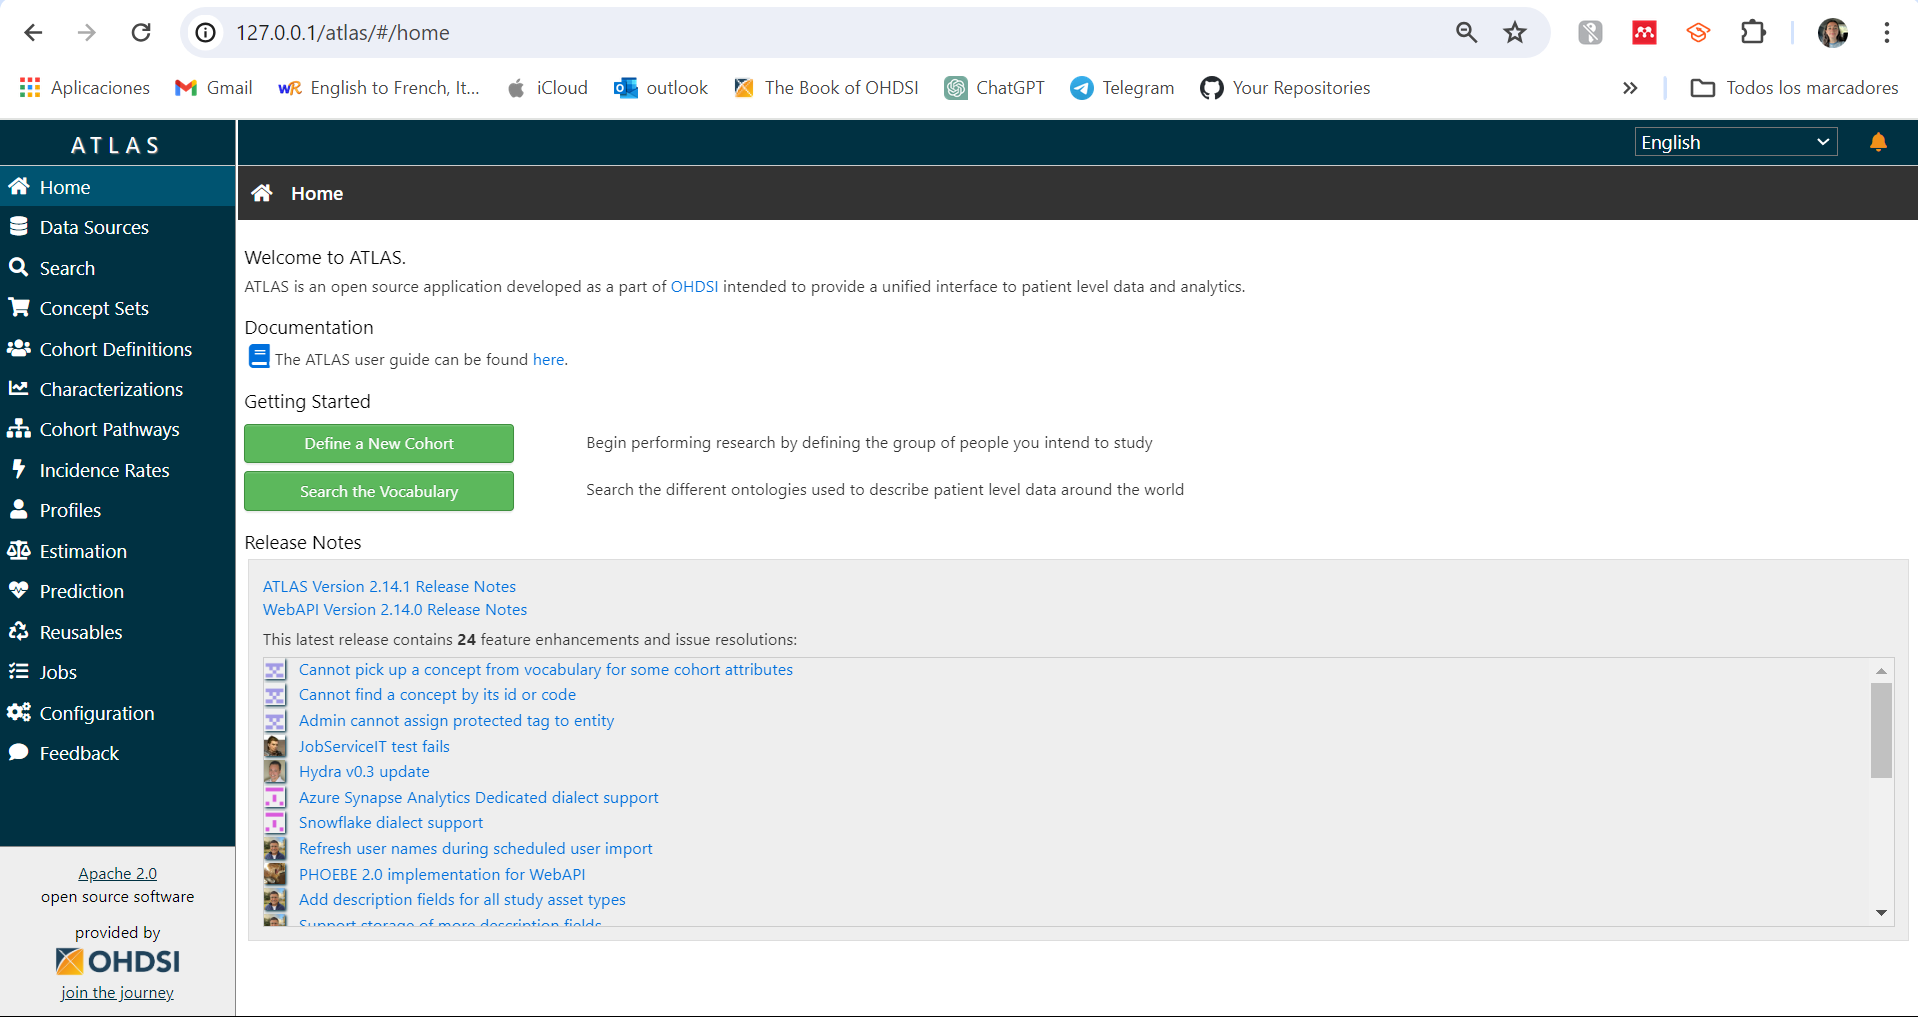
\includegraphics[width=0.90\textwidth]{figures/homeATLAS.png}
     \caption{Captura de pantalla del menú principal de ATLAS Broadsea}
    \label{fig:homeATLAS}
\end{figure}

El menú lateral de ATLAS presenta 15 herramientas de análisis, de las cuales en el proyecto se utilizan las siguientes:

\begin{itemize}
    \item \textbf{Home}. Es el menú principal de ATLAS. Se muestra por defecto al abrir la herramienta.
    \item \textbf{Data Sources}. Es la herramienta para obtener reportes de las bases de datos integradas en la herramienta.
    \item \textbf{Search}. Es la herramienta para realizar búsquedas de conceptos en el Vocabulario.
    \item \textbf{Concept Sets}. Es la herramienta para definir grupos de conceptos que se utilizarán en la realización de análisis.
    \item \textbf{Cohort Definitions}. Es la herramienta para definir las cohortes que intervienen en los estudios y análisis.
    \item \textbf{Characterization}. Es la herramienta para realizar estudios estadísticos de caracterización de las cohortes definidas.
    \item \textbf{Estimation}. Es la herramienta para realizar estudios de estimación a nivel de población.
    \item \textbf{Prediction}. Es la herramienta para realizar estudios de predicción a nivel de paciente.
\end{itemize}

ATLAS Broadsea despliega por defecto la base de datos de Eunomia, que es una pequeña base de datos sintética estructurada al Modelo Común de Datos de OMOP que sirve de ayuda para la toma de contacto con la herramienta. La base de datos de Broadsea es accesible a través de un gestor de bases de datos PostgreSQL como pgAdmin. A continuación se muestra la estructura del servidor y base de datos de Broadsea.

\begin{figure}[H]
\centering
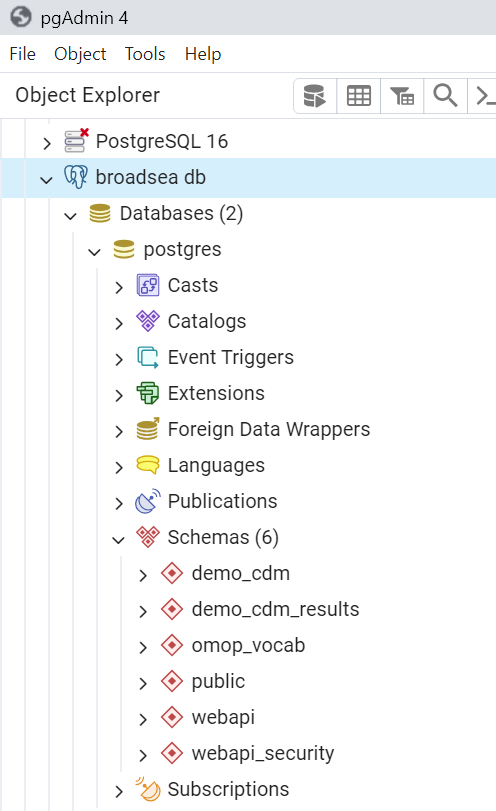
\includegraphics[width=0.50\textwidth]{figures/serverBroadsea.png}
     \caption{Captura de pantalla de pgAdmin de la estructura del servidor de Broadsea}
    \label{fig:serverBroadsea}
\end{figure}

La base de datos presenta seis esquemas, siguiendo la configuración del Modelo de Datos Común de OMOP \parencite{githubCDMConfig}. Para mayor información sobre la estructura postgre de Broadsea se recomienda consultar el anexo \ref{anexo:manual} ''Manual de instalación, despliegue y configuración de ATLAS Broadsea''. No obstante, a continuación se describe brevemente la función de cada uno de estos esquemas:

\begin{itemize}
    \item \textbf{demo\_cdm:} Contiene toda la información de eventos clínicos y pacientes registrados en la base de datos. Es el grueso del contenido de la base de datos.
    \item \textbf{demo\_cdm\_results:} Contiene información generada de la ejecución de ACHILLES (véase \ref{sec:07herramientas} ''Herramientas de OHDSI'') sobre la base de datos.
    \item \textbf{omop\_vocab:} Este esquema no venía preinstalado pero es fundamental para el correcto funcionamiento de la herramienta. Contiene todo el vocabulario que va a ejecutar ATLAS. Su intalación se detalla en el manual.
    \item \textbf{public:} Este esquema no pertenece al CDM sino que se genera por defecto al crear una base de datos postgre. No contiene información relevante.
    \item \textbf{webapi:} Es el esquema de la WebAPI. Desde este esquema se establecen y gestionan las conexiones con bases de datos externas.
    \item \textbf{webapi\_security:} Este esquema contiene ajustes para configurar la seguridad de la WebAPI. No se utiliza en el proyecto. Mayor información sobre la seguridad de la WebAPI en el manual.
\end{itemize}


\section{Conclusiones} \label{sec:08conclusiones}

En este capítulo se concluye que la arquitectura tecnológica del sistema es compleja puesto que involucra una virtualización del ecosistema OHDSI a través de Docker, denominado Broadsea. No obstante, la implementación del sistema en Docker facilita bastante la tarea de configurar el ecosistema completo, gracias al empaquetamiento de las funcionalidades en contenedores accesibles \textit{a-la-carte}. 
    \chapter{Caso práctico}\label{cap:09caso}
En este capítulo se presenta: \ref{sec:09intro} Introducción al caso práctico, \ref{sec:09huvr} El estudio realizado por el Hospital Universitario Virgen del Rocio, \ref{sec:09atlas} El estudio realizado utilizando ATLAS, \ref{sec:09resultados} Discusión de resultados y \ref{sec:09conclusiones} Conclusiones.

\section{Introducción} \label{sec:09intro}

Este capítulo pretende demostrar la relevancia de OHDSI (Observational Health Data Science and Informatics) y la utilidad de sus herramientas, concretamente el uso de ATLAS para la estandarización y reproducibilidad de los análisis clínicos observacionales sobre bases de datos estandarizadas al Modelo de Datos Común de OMOP. 

Para ello, bajo la tutela de D. Carlos Parra y Da. Silvia Rodríguez (tutores de las prácticas en empresa, véase \ref{sec:03Participantes} ''Participantes del proyecto''), se ha seguido la reproducción de un estudio realizado por investigadores del hospital sobre predicción mediante modelos de ML de efectos adversos en el tratamiento radioterápico de pacientes con cáncer de pulmón. 

Este estudio, se encuentra públicamente accesible en Pubmed en dos artículos, el primero publicado en el año 2019 titulado \textit{''Comparison of Feature Selection Methods for Predicting RT-Induced Toxicity'' }\cite{nunez2019comparison} y el segundo, en 2023 titulado \textit{''Benchmarking machine learning approaches to predict radiation-induced toxicities in lung cancer patients''} \cite{nunez2023benchmarking}. Ambos estudios están también publicados en la ruta \code{Thesis-ATLAS-OHDSI/documentation/pdf/estudioHUVR} del repositorio de github del TFG \cite{vallealonsodc}.

El objetivo es promover el uso de ATLAS para la investigación observacional, reproduciendo mediante ATLAS un estudio que fue realizado sin hacer uso de la herramienta, para demostrar con un caso práctico los beneficios de utilizar la herramienta en términos de reproducibilidad y estandarización.

\section{Estudio realizado por el HUVR} \label{sec:09huvr}

El estudio consiste en la comparación de 300 modelos de ML sobre un dataset de 875 pacientes de cancer de pulmón con el objetivo de predecir los efectos adversos a corto (esofagitis, tos, disnea y neumonitis) y a largo plazo (disnea y neumonitis) que producirá el tratamiento radioterápico sobre estos pacientes. 

\subsubsection{Contexto}

%La base teórica del estudio \cite{nunez2019comparison, nunez2023benchmarking} es que la radioterapia aunque es beneficiosa para el tratamiento oncológico, también causa efectos perjudiciales a corto y/o  largo plazo de forma personalizada según las condiciones de cada paciente. El auge de la medicina personalizada y centrada en el paciente (véase \ref{sec:01Contexto}) ha ensalzado la importancia de realizar una planificación individual para cada paciente, pues cada persona responde de forma distinta a los tratamientos. Por tanto, la gestión individualizada de los posibles efectos adversos es muy importante en la planificación del tratamiento radioterápico, con el fin de facilitar la toma de decisiones entre médico y paciente en términos de calidad de vida y posibilidades de supervivencia.

La radioterapia, aunque beneficia el tratamiento oncológico, puede ocasionar efectos perjudiciales a corto y largo plazo, de forma personalizada según cada paciente \cite{nunez2019comparison, nunez2023benchmarking}. La medicina centrada en el paciente (véase \ref{sec:01Contexto} ''Marco contextual'') destaca la importancia de planificar individualmente cada tratamiento, dado que las respuestas varían entre individuos. Por tanto, la gestión personalizada de los efectos adversos es crucial en la planificación radioterápica para facilitar la toma de decisiones médico-paciente en términos de calidad de vida y supervivencia.

\subsubsection{Objetivo}

El objetivo del estudio es utilizar un conjunto de datos del mundo real (RWD) para facilitar la toma de decisiones clínicas, estudiando para cada efecto adverso del tratamiento radioterápico, el modelo de ML que provee una mejor predicción en términos de precisión del modelo (AUC).

\subsubsection{Datos}

- RWHD

\textcolor{red}{- 875 pacientes del registro s31 y observacion del huvr??}

\subsubsection{Metodología}

Para conformar los 300 modelos de ML se han entrenado y testeado 5 modelos de ML combinados con 10 métodos de selección de atributos (\textit{Feature Selection, FS}) sobre 6 efectos adversos (\textit{outcomes} o \textit{clinical endpoints}), de la siguiente forma: 

\begin{itemize}
    \item \textbf{5 Modelos de ML}. Se utilizaron cinco clasificadores basados en aprendizaje 
    automático: 
    \begin{itemize}[label={--}]
        \item Máquina de Vectores de Soporte (\textit{Support Vector Machine, SVM}).
        \item Vecinos más Cercanos (\textit{k-Nearest Neighborhood, kNN}).
        \item Red Neuronal Artificial (\textit{Artificial, Neural Network, ANN}) de alimentación directa.
        \item Modelo Lineal Generalizado (\textit{Generalized Linear Model, GLM}).
        \item Clasificador de Naïve-Bayes (\textit{NB}).
    \end{itemize}
     Los hiperparámetros de los modelos se se optimizaron automáticamente siguiendo ''las recomendaciones de la literatura''.
    
    \item \textbf{10 Métodos de Selección de Atributos \textit{(FS)}.} Para reducir la dimensionalidad de los conjuntos de datos, se implementaron los siguientes métodos:
    
    \begin{itemize}[label={--}]
        \item Selección de Características Basada en Correlación (\textit{Correlation-based Feature Selection, CFS}).
        \item Chi-cuadrado %(\( \chi^2 \)).
        \item Boruta.
        \item Mínima Redundancia - Máxima Relevancia (\textit{Minimum Redundancy-Maximum Relevance, mRMR}).
        \item Relief.
        \item Ganancia de Información (\textit{Information Gain, IG}).
        \item  Bosque Aleatorio (\textit{Random Forest, RF}).
        \item 2 métodos de ensamblaje a partir de métodos de FS individuales y de subconjuntos.
        \item Subconjuntos de variables determinadas por un oncólogo experto para predecir las toxicidades seleccionadas basadas en la evidencia clínica.
    \end{itemize}

    \item \textbf{6 Efectos adversos.} Se seleccionaron seis efectos adveros a estudiar, clasificados según si su duración fue a corto plazo y a largo plazo. A corto plazo:
    \begin{itemize}[label={--}]
        \item Esofagitis.
        \item Tos.
        \item Disnea. 
        \item Neumonitis. 
    \end{itemize}
    A largo plazo:
    \begin{itemize}[label={--}]
        \item Disnea. 
        \item Neumonitis. 
    \end{itemize}
    Se consideran efectos adversos crónicos o a largo plazo si los efectos se mantuvieron presente más de tres meses a partir del inicio del tratamiento.
\end{itemize}

Para la validación interna de los modelos se ha utilizado una estrategia de validación cruzada de 10 pliegues (\textit{10-fold Cross-Validation}) en la que se aplicó una técnica de submuestreo aleatorio para generar un conjunto de datos equilibrado. Para la validación externa, se han utilizado los datos generados con los casos registrados después del 31 de mayo de 2018, que no fueron utilizados para la validación interna. 

Por último, el rendimiento de los modelos se ha medido en términos del AUC logrado por cada modelo predictivo.

\subsubsection{Resultados}

   Los resultados del estudio resaltan para cada outcome el mejor modelo de ML y selección de atributos, con la valoración de AUC en validación interna y externa. Los resultados se muestran de forma muy intuitiva en la siguiente tabla, extraída del artículo del HUVR \cite{nunez2023benchmarking}.

\begin{figure}[H]
    \centering
    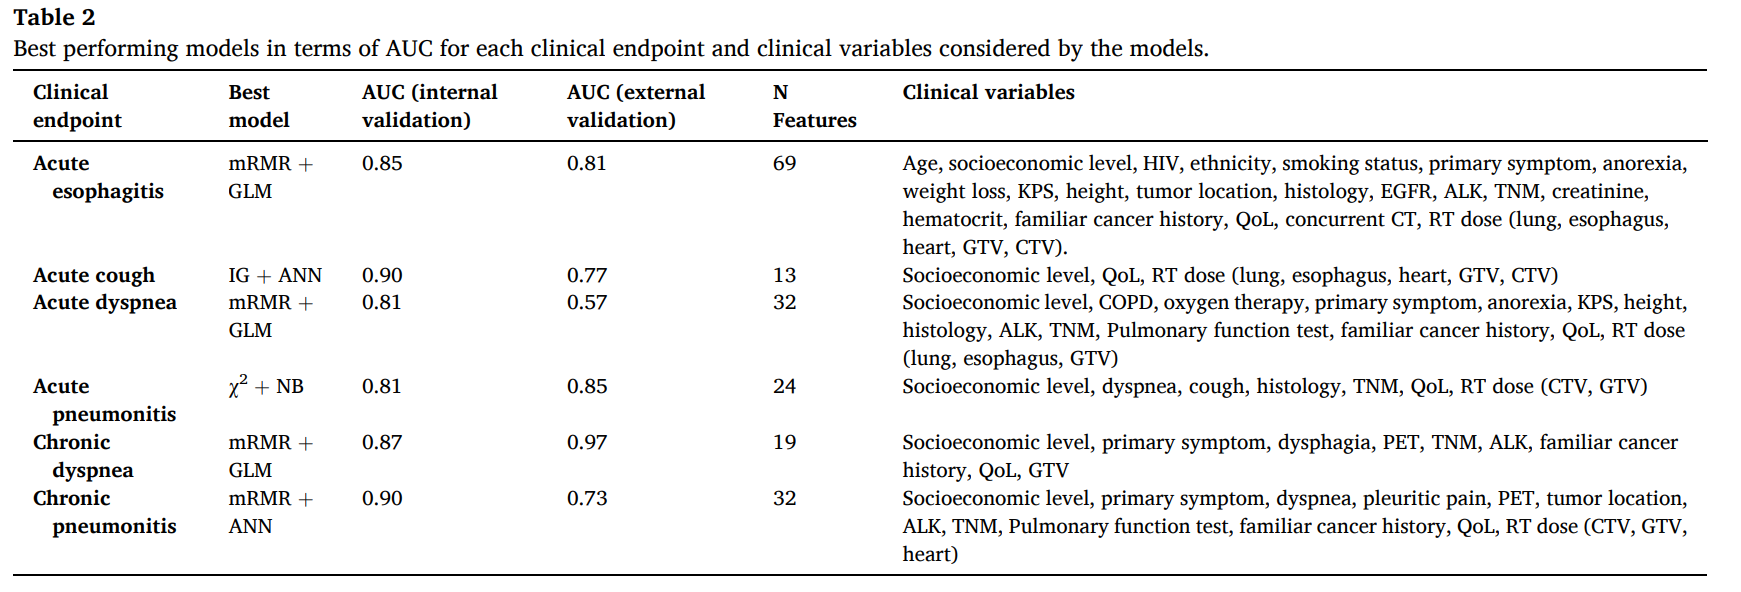
\includegraphics[width=1\textwidth]{tables/nune2023table2.png}
    \captionof{table}{Recopilación de resultados. Extraída de \cite{nunez2023benchmarking}}
    \label{table:nune2023table2}
\end{figure}


\section{Reproducción del estudio con ATLAS} \label{sec:09atlas}
%Caso práctico del TFG

%Check de los casos de uso/requisitos en el estudio real.

- Reinterpretación del estudio

\subsection{Datos}
%\subsection{Comprobación calidad datos}

%- Datos omopizados por TFG Paco 
%- Calidad previa y post comprobada tb en TFG Paco

Se han obtenido el dataset que se utilizó en ese estudio.

- Los datos se convirtieron a OMOP (TFG Paco)

- Se analizó la calidad de los datos eficiente (TFG Paco)

\subsection{Metodología}


\subsubsection{Reporte del dataset}

\subsubsection{Definición de grupos de conceptos}

\subsubsection{Definición de cohortes}

Necesario para utilzar ATLAS

Cohorte = Personas con cancer de pulmon

\subsubsection{Caracterización}

Para conocer los pacientes que tenemos en el cohorte

\subsubsection{Estimación a nivel de población}

Hacer un estudio sobre los efectos adversos que sufrirá la población del cohorte

\subsubsection{Predicción a nivel de Paciente}

Para un paci

\subsection{Resultados}


\section{Discusión de resultados} \label{sec:09resultados}

%Aqui son resultados concretos del estudio. En la sección de resultados serán resultados compeltos del TFG

Comparación de los resultados obtenidos en el estudio del HUVR y el estudio realizado con ATLAS


\section{Conclusiones} \label{sec:09conclusiones}

En este capítulo se concluye que...
    \chapter{Resultados}\label{cap:10resultados}

\section{Resultados}

- Muchos problemas

\section{Trazabilidad de objetivos}

Trazabilidad de objetivos con resultados

\section{Lecciones aprendidas}

- Comprensión de la importancia de la estandarización (estandar OHDSI) en la interoperabilidad de los sistemas clínicos.

- Implementación de un entorno virtual en el PC (Entorno y webAPI de OHDSI en MV DOCKER)

- Aprendizaje de uso de la herramienta ATLAS

- Limitacion temporal a la hora de realizar el estudio

- Limitaciones por autoaprendizaje de las interfaces y herramientas
    \chapter{Conclusiones}\label{cap:11conclusiones}




    %\bibliographystyle{apacite}
    %\bibliographystyle{unsrtnat}
    %\bibliography{bibliografia.bib}
    \printbibliography

    \appendix
    \chapter{Manual de ATLAS Broadsea}\label{anexo:manual}

El nombre completo de este anexo corresponde a \textbf{Manual de instalación, despliegue y configuración de ATLAS Broadsea}, aunque por motivos de extensión se ha reducido en el índice de la memoria a \textit{Manual de ATLAS Broadsea}.

El manual se presenta a la convocatoria como un documento aparte debido a su larga extensión, de casi 40 páginas. No obstante, se utiliza este apartado de la memoria para presentar resumidamente sus contenidos básicos y cómo acceder a él. Su gran extensión se debe a a que recopila en un único lugar una grandísima variedad de información que hasta ahora se encontraba esparcida de forma más o menos ordenada en la red, sobretodo en diferentes repositorios de github. 

El anexo se adjunta a la documentación entregable de la convocatoria con el nombre ''Anexo A - Manual de ATLAS Broadsea.pdf''. Adicionalmente, también es accesible a través del repositorio de github del Trabajo Fin de Grado \cite{vallealonsodc}, concretamente en la ruta \code{Thesis-ATLAS-OHDSI/documentation/pdf}.

%El manual es un documento de gran valor debido a que recopila en un único lugar una grandísima variedad de información que hasta ahora se encontraba esparcida de forma más o menos ordenada en la red, pero nunca recopilada en un único documento. Su redacción como un documento aparte nace de la propia dificultad a la que se enfrenta la alumna a la hora de instalar, desplegar y configurar la herramienta para la reproducción del estudio práctico con el fin de facilitar a futuros usuarios y a sus propios compañeros del departamento de Innovación Tecnológica del Hospital Universitario Virgen del Rocío una guía detallada con todos los contenidos necesarios para replicar esta tarea cuando fuere necesario.

El manual trata cinco aspectos importantes de ATLAS Broadsea: 

\begin{enumerate}
    \item \textbf{Introducción y descripción de Broadsea.} Este capítulo explica contenidos sobre el entorno tecnológico necesario para seguir correctamente los procedimientos del manual.
    \item \textbf{Despliegue por defecto.} Este capítulo presenta el despliegue más sencillo del entorno Broadsea, sin ningún tipo de configuración adicional.
    \item \textbf{Conexión con la BD por defecto.} Este capítulo explica la conexión con el servidor Postgre del contenedor docker de Broadsea.
    \item \textbf{Conexión con BD externa.} Este capítulo explica cómo añadir una conexión de una base de datos externa al servidor docker de Broadsea.
    \item \textbf{Configuración del Vocabulario.} Eeste capítulo explica cómo configurar el Vocabulario desde ATHENA y se presentan otras configuraciones avanzadas.
\end{enumerate}

Todo ello complementa la información del TFG de forma subyacente, es decir, durante la reproducción del estudio práctico (véase \ref{cap:08pruebas}) se da por supuesto todo el proceso de instalación de la herramienta así como la configuración del servidor, base de datos, étc. En términos de roles del proyecto (véase \ref{cap:03gestión}) se podría decir que mientras que el analista se encarga de reproducir el estudio haciendo uso de la interfaz de usuario de ATLAS, el developer habría sido el encargado de realizar toda el anexo, con toda la instalación, despliegue y configuración para que la herramienta funcione. No obstante, en este caso ambos roles son ejecutados por la misma persona que es la alumna. Además satisface explícitamente el \textbf{Obj-002} del Trabajo Fin de Grado (véase \ref{cap:02objetivos}).




    \chapter{Glosario}\label{anexo:glosario}


\textbf{Aprendizaje automático (\textit{Machine Learning, ML}):} Campo de la inteligencia artificial que desarrolla algoritmos y modelos que permiten a las máquinas aprender a partir de datos, identificar patrones y tomar decisiones sin necesidad de ser programadas explícitamente para cada tarea específica.

\textbf{ATLAS}: Herramienta de código abierto desarrollada por la colaboración Observational Health Data Sciences and Informatics (OHDSI), diseñada para la visualización, exploración y análisis de datos de salud provenientes de diferentes fuentes y estándares, facilitando la investigación en salud pública y la toma de decisiones clínicas basadas en evidencia.


%%B

%\textbf{\textit{Backend}}: Parte de un sistema de software que se encarga del procesamiento y la gestión de datos, así como de la lógica de negocio que no es visible para el usuario final. Incluye el servidor, la base de datos y la lógica de aplicación que realiza las operaciones detrás de escena para proporcionar funcionalidades al frontend.

%%C

\textbf{Código abierto \textit{(Open source)}}: Modelo de desarrollo de software que promueve el acceso abierto al código fuente de un programa, permitiendo su estudio, modificación y distribución por parte de la comunidad de desarrolladores, lo que fomenta la colaboración, la transparencia y la innovación en el desarrollo de software.

\textbf{Cohorte \textit{(Cohort)}}: Grupo de individuos que comparten una característica común o que han sido seleccionados para participar en un estudio de investigación, con el fin de observar y analizar los resultados de un evento o exposición específica durante un período de tiempo determinado.

\textbf{Computación en la Nube (\textit{Cloud Computing}):} Modelo de prestación de servicios de computación a través de internet, donde los recursos como almacenamiento, servidores y aplicaciones son proporcionados y gestionados por proveedores externos, permitiendo un acceso flexible y escalable según la demanda del usuario.

\textbf{Contenedor Docker \textit{(Docker container)}}: Tecnología de virtualización que permite empaquetar y ejecutar aplicaciones y sus dependencias en entornos aislados, proporcionando portabilidad, rapidez y consistencia en el despliegue de aplicaciones en diferentes sistemas operativos y entornos de ejecución.



%%D

\textbf{Datos del mundo real \textit{(Real World Data, RWD)}}: Información sobre la salud y los resultados de atención médica recopilada de fuentes del mundo real, como registros médicos electrónicos, reclamaciones de seguros y dispositivos portátiles, utilizada para complementar los datos de ensayos clínicos y proporcionar información sobre la efectividad y seguridad de tratamientos en condiciones reales fuera del entorno controlado de un estudio clínico.

\textbf{Datos masivos (\textit{Big Data}):} Conjunto de datos extremadamente grandes y complejos que requieren tecnologías especializadas para su almacenamiento, procesamiento y análisis, con el objetivo de extraer información significativa y tomar decisiones informadas.


%%E

\textbf{\textit{European Health Data \& Evidence Network (EHDEN)}}: Consorcio europeo que tiene como objetivo establecer una infraestructura escalable y sostenible para el análisis de datos de salud del mundo real en Europa. EHDEN promueve la estandarización de datos y el uso de herramientas y métodos avanzados para facilitar la investigación clínica y epidemiológica.

%%F

%\textbf{\textit{Frontend}}: Nivel de un sistema de software o una aplicación que interactúa directamente con el usuario final. Incluye la interfaz de usuario, que permite a los usuarios interactuar con el sistema, y cualquier elemento visible o interactivo en la pantalla, como botones, formularios y gráficos. 

%%G

%%H

\textbf{Historial Clínico Electrónico (HCE)}: Registro digitalizado y centralizado de toda la información médica de un paciente, que incluye datos como diagnósticos, tratamientos, resultados de pruebas, alergias y antecedentes médicos, accesible por profesionales de la salud autorizados para mejorar la coordinación de la atención, la precisión diagnóstica y la seguridad del paciente.




%%I
\textbf{Industria 4.0 (\textit{Industry 4.0}):} Concepto acuñado por el gobierno alemán en 2011 para referirse a la emergente cuarta revolución industrial basada fundamentalmente en la integración de los sistemas físicos con Internet a través de herramientas como Internet de las cosas, Big Data, Cloud Computing o Inteligencia Artificial.

\textbf{Inteligencia Artificial (\textit{Artificial Intelligence, AI}):} Disciplina científica que se ocupa de crear programas informáticos que ejecutan operaciones comparables a las que realiza la mente humana, como el aprendizaje o el razonamiento lógico.

\textbf{Internet de las cosas (\textit{Internet of Things, IoT}):} Red de dispositivos, sistemas y servicios que incorporan sensores, software y otras tecnologías que permiten la conectividad avanzada y el intercambio de datos entre sí a través de Internet u otras redes de comunicación.


\textbf{Interoperabilidad}: Capacidad de sistemas, dispositivos o aplicaciones para intercambiar datos y trabajar juntos de manera efectiva, garantizando que la información sea comprensible y utilizada de manera consistente entre diferentes plataformas, organizaciones o entornos. Se puede clasificar en tres grupos: semántica, técnica y organizacional.

%%J

%%K

%%L


\textbf{\textit{Low-code}}: Enfoque de desarrollo de software que utiliza herramientas visuales y abstracciones de código para permitir a los usuarios crear aplicaciones de manera rápida y con menos necesidad de programación manual, acelerando el proceso de desarrollo y permitiendo a usuarios con menos experiencia técnica participar en la creación de aplicaciones.

%%M

\textbf{Modelo de Datos Común de OMOP \textit{(OMOP Common Data Model, OMOP CDM)}}: Estructura estandarizada de base de datos desarrollada por la colaboración Observational Medical Outcomes Partnership (OMOP), diseñada para representar datos de salud de manera uniforme y compatible, facilitando el análisis comparativo de datos clínicos y epidemiológicos provenientes de diferentes fuentes y sistemas de salud.


%%N

%%Ñ

%%O
\textbf{\textit{Observational Health Data Sciences and Informatics (OHDSI)}}: Organización internacional que desarrolla y aplica métodos de análisis de datos de salud para generar evidencia a partir de datos del mundo real, con el objetivo de mejorar la toma de decisiones en salud pública y clínica, promoviendo el uso de estándares y herramientas abiertas para el intercambio y análisis de datos.

\textit{\textbf{Observational Medical Outcomes Partnership (OMOP)}}: Iniciativa colaborativa entre la industria, académicos y reguladores para mejorar la evaluación de medicamentos a través del análisis de datos de salud del mundo real. OMOP desarrolla métodos y estándares para el análisis de datos de salud, incluido el Modelo de Datos Común (CDM), que permite la armonización de datos para la investigación.

\textbf{OMOPizar}: Proceso de transformar datos de salud de diferentes fuentes y formatos al Modelo de Datos Común de OMOP (CDM), para estandarizar la representación de los datos y facilitar su análisis comparativo y la generación de evidencia científica en investigación clínica.



%%P

%%Q

%%R

%%S

\textbf{Salud digital \textit{(e-Salud)}}: Utilización de tecnologías de la información y comunicación en el ámbito de la salud para mejorar la eficiencia, accesibilidad, calidad y seguridad de los servicios médicos, así como para fomentar la participación activa de los pacientes en su cuidado y la gestión de su salud.

\textbf{Sanidad 4.0 (\textit{Healthcare 4.0})}: También conocido como Salud 4.0, es la aplicación de tecnologías digitales como inteligencia artificial, Internet de las cosas y big data en el sector de la salud para mejorar la atención médica, la gestión de datos y la experiencia del paciente.

\textbf{Sistemas ciber-físicos (\textit{Cyber-Physical Systems, CPS}}): Sistemas que integran componentes físicos y computacionales, conectados a través de redes, para monitorear y controlar procesos físicos en tiempo real, utilizando tecnologías como sensores, actuadores, y sistemas de información y comunicación.



%%T

\textbf{Tecnologías de la Información y Comunicación (TICs)}: Conjunto de herramientas, recursos y sistemas tecnológicos utilizados para adquirir, almacenar, procesar, transmitir y presentar información de manera digital, facilitando la comunicación y el intercambio de datos entre personas, organizaciones y dispositivos.

\textbf{Telemedicina}: Práctica médica que utiliza tecnologías de la información y comunicación para realizar consultas médicas, diagnósticos, tratamiento y seguimiento de pacientes a distancia, facilitando el acceso a la atención médica y la colaboración entre profesionales de la salud sin necesidad de encuentros físicos.

%%U

%%V

%%W

%%X

%%Y

%%Z




% Fin del documento
\end{document}
